\NeedsTeXFormat{LaTeX2e}
\documentclass[final]{jfp1}

\usepackage{xspace, graphicx, placeins}  
\usepackage[title, titletoc]{appendix}
\usepackage[usenames, dvipsnames]{xcolor}
\usepackage{listings}
\lstset{language=erlang, basicstyle=\small\ttfamily, columns=flexible}
\usepackage{tikz, pgfplots}
\usepackage{stmaryrd, amssymb}
\usepackage{subfigure}
\usepackage{algorithm}
\usepackage{algorithmic}
\usepackage{listings}
\usepackage{array}
\usepackage{tabularx}
%\usepackage{mathtools}
\usepackage{amsfonts}
\usepackage{lscape}
\usepackage{stmaryrd}
\usepackage{amsmath,amssymb}
%\usepackage{listings}
\usepackage{graphicx}
\usepackage{graphics,epsfig,alltt}
\usepackage[official,right]{eurosym}
\usepackage{xspace} % to allow automatic spacing of the \Paraphrase acronym but still observing punctuation.
\usepackage{url}
\usepackage{mathpartir}
\usepackage{semantic}


\usepackage{xspace, dashrule, float}
\usepackage{rotating}

%\usepackage{listings}
\lstset{language=erlang, basicstyle=\small\ttfamily, columns=flexible, frame=tb}

%%% Macros for the guide only %%%
\providecommand\AMSLaTeX{AMS\,\LaTeX}
\newcommand\eg{\emph{e.g.}\ }
\newcommand\etc{\emph{etc.}}
\newcommand\bcmdtab{\noindent\bgroup\tabcolsep=0pt%
  \begin{tabular}{@{}p{10pc}@{}p{20pc}@{}}}
\newcommand\ecmdtab{\end{tabular}\egroup}
\newcommand\rch[1]{$\longrightarrow\rlap{$#1$}$\hspace{1em}}
\newcommand\lra{\ensuremath{\quad\longrightarrow\quad}}

\newcommand{\memo}[1]{\emph{\color{MidnightBlue} [#1]}}
\newcommand{\ra}[0]{$\rightarrow$\xspace}

\newcommand{\func}[0]{\texttt{func}\xspace}
\newcommand{\pipe}[0]{\texttt{pipe}\xspace}
\newcommand{\farm}[0]{\texttt{farm}\xspace}
\newcommand{\cluster}[0]{\texttt{cluster}\xspace}
\newcommand{\ord}[0]{\lstinline{ord}\xspace}
\newcommand{\map}[0]{\lstinline{map}\xspace}
\newcommand{\reduce}[0]{\lstinline{reduce}\xspace}
\newcommand{\fback}[0]{\lstinline{feedback}\xspace}

\newcommand{\ee}[0]{\hspace{1em} \mathcal{E}}
\newcommand{\opt}[0]{\hspace{1em} \oplus \, \mathcal{E}}
\newcommand{\qq}[1]{\llbracket\, \mathtt{#1}\,\rrbracket}
\newcommand{\qquote}[1]{\llbracket\, #1 \,\rrbracket}
\newcommand{\cond}[1]{\hspace{1em} \{ #1 \}}
\newcommand{\inenv}[1]{#1 \in \rho}
\newcommand{\ninenv}[1]{#1 \not\in \rho}
%\newcommand{\comp}[0]{\, \circ \,}

%% Refactoring Notation definitions
\newcommand{\f}[0]{\bar{f}}
\newcommand{\s}[0]{\bar{s}}
\newcommand{\blf}[0]{\mathbb{F}}
\newcommand{\bs}[0]{\mathbb{S}}
\newcommand{\bn}[0]{\mathbb{N}}
\newcommand{\br}[0]{\mathbb{R}}
\newcommand{\bnp}[0]{\bn^{+}}
\newcommand{\bnz}[0]{\bn^{0}}
\newcommand{\brp}[0]{\br^{+}}
\newcommand{\type}[3]{#1: #2\; #3}
\newcommand{\ing}[1]{#1 \in{} \Gamma}

\newcommand{\seq}[3]{#1 & \vdash{} & #2 & = & #3}
\newcommand{\rewrite}[3]{#1 & \vdash{} & #2 & \mapsto{} & #3}
\newcommand{\Rewrite}[3]{#1 & \vdash{} & #2 & \mapsto{}^{\!\!\!*} & #3}

\newcommand{\ie}[0]{i.e.\@\xspace}

\newcommand{\lapedo}{\xspace{\sc Lapedo}\xspace}
\newcommand{\Lapedo}{\lapedo}

\makeatletter
\def\thickhrulefill{\leavevmode \leaders \hrule height 0.5pt \hfill \kern \z@}
\newcommand{\hrules}{\vspace{1.5ex}\thickhrulefill}
\newcommand{\hrulee}{\thickhrulefill\vspace{1.5ex}}

\newcommand{\stream}[1]{~<\!\!<#1>\!\!>~}

\title[Refactoring for Heterogeneous Parallelism in Erlang]
      {Refactoring for Introducing and Tuning Parallelism For Heterogeneous Multicore Machines in Erlang}

 \author[V. Janjic et al]{VLADIMIR JANJIC, CHRISTOPHER BROWN, ADAM BARWELL \\
         University of St Andrews, School of Computer Science, UK\\
%         \email{\{vj32,cmb21,adb23,kh8\}@st-andrews.ac.uk}}
         \email{vj32@st-andrews.ac.uk, cmb21@st-andrews.ac.uk, adb23@st-andrews.ac.uk, kevin@kevinhammond.net} 
}         
\author[K. Hammond]{KEVIN HAMMOND \\ Hylomorph Solutions, Glasgow, UK \\
	\email{kevin@kevinhammond.net}
}

\jdate{September 2001, update April 2007}
\pubyear{2001}
\pagerange{\pageref{firstpage}--\pageref{lastpage}}
\doi{S095679680100457}

\newtheorem{lemma}{Lemma}[section]

\begin{document}

\label{firstpage}

\maketitle

\begin{abstract}
  This paper presents semi-automatic software refactorings to introduce and tune structured parallelism in sequential Erlang code, as well as to generate code for running computations on accelerators such as GPUs. Our refactorings are based on the \Lapedo{} framework for programming
  \emph{heterogeneous} multi-core systems in Erlang. \Lapedo{} utilises a set of \emph{hybrid
  skeletons} that contain components for different processor types, together with novel \emph{refactorings} for introducing and tuning parallelism together with generating cumbersome boilerplate code for offloading and scheduling 
  computations on different processors.
  We demonstrate, on four realistic use-case applications, that we are able to refactor 
  sequential code and produce heterogeneous parallel versions that can achieve significant and scalable speedups of up to 220
  over the original sequential Erlang program on a 24-core
  machine with a GPU. % for the particular application.
%   \keywords{Erlang; Parallel Skeletons; Parallel Refactoring;
%     Heterogeneous Multi-core Systems.}
\end{abstract}

%\tableofcontents

\section{Introduction}
\vspace{-6pt}
%CB: scheduling vs. mapping
\noindent
Following initial stages of multi-core revolution, another big change has happened in the computer hardware world. Emergence of
\emph{accelerators}, such as graphic processing units (GPUs),
field programmable gate arrays (FPGAs) and Intel Xeon PHIs, has
resulted in a new class of devices, \emph{heterogeneous multi-cores/many-cores}.
These systems combine traditional multi-core CPUs with one or more
accelerators, and are nowadays found in almost all high-performance systems,
desktops, clouds, gaming consoles, tablets and mobile phones.
These systems
offer a significant computing potential that can deliver orders of magnitude
more performance than traditional CPU-only based systems, and almost all
of them support execution of \emph{general-purpose} parallel applications.

However, we know that nothing comes for free. In order to fully exploit
the potential that the heterogeneous multi-core/many-core systems offer, a programmer needs
to combine different low-level programming models, e.g.~CUDA or OpenCL for GPUs,
WHDL or Verilog for FPGAs and OpenMP for CPUs. This involves
combining different models for CPUs and different 
accelerators, explicitly manage data transfers between main memory and
accelerator memory, schedule computations on the accelerators, fetch the 
results back etc. 
Moreover, solutions
that perform well are usually tied to a specific heterogeneous architecture
and cannot easily be ported, yielding problems in terms of e.g. increased maintainance and lack of longevity.
This makes programming heterogeneous many-core systems much
harder than is alredy very-hard task of programming multi-core CPUs. What is
needed are high-level programming models that will hide both hardware 
complexity of such systems, and also different models required to program them,
while still achieving the performance comparable to that of hand-crafted
low-level code. Functional programming, allowing a very high-level of 
abstraction without having to worry about the actual program flow, sounds
like an ideal fit to program these systems. However, bridging the gap between
high-level of abstraction and a complexity of the underlying hardware and
programming models for it has so far proven to be a too big obstacle.

In our previous work~\cite{parco2015}, we have introduced the novel \Lapedo{} framework for programming heterogeneous multi-core systems in Erlang. \Lapedo{} is based on \emph{hybrid skeletons} that can be used to abstract across low-level programming details. In this paper, we extend this framework with novel \emph{refactorings} (programmer-directed source-level transformations). The extended framework enables the  programmer to firstly focus on finding  the most appropriate parallel \emph{structure} for their application, and then on ensuring good, portable performance across a range of heterogeneous multicores. Given a OpenCL kernel, which the programmer has written by hand, \Lapedo{} automatically generates the tedious and error-prone code for creating buffers on accelerators, transferring the data to/from them, setting the  necessary parameters, scheduling the execution of computations on accelerators, fetching the results back and so on. Furthermore, it semi-automatically, under the programmer's guidance, introduces calls to instances of hybrid skeletons into the sequential code after, also semi-automatically, shaping the code in order to choose e.g.~the most appropriate data structures for the underlying hybrid skeleton.

% Refactoring allows the programmer to apply well-defined
% rules that transform their code step-by-step, starting from a sequential
% version to the final parallel version. It also allows user to provide
% input and steer the process of parallelisation.
% In our previous work~\cite{homskel}, we have described an
% initial Skel version that contains only \emph{homogeneous} skeletons,
% i.e.\ skeletons that can contain only CPU components. In this paper,
% we present the extension of the Skel to adapt it to heterogeneous
% systems, and a set of new refactorings for managing code for these
% systems. In particular, 
The paper makes the following main research contributions:
\begin{enumerate}
%\item We extend the \emph{Skel} Erlang library of parallel skeletons with
%\emph{hybrid skeletons} that allow combining of CPU and accelerator 
%components within the same skeleton;
%We introduce the first portable, high-level \emph{hybrid skeletons} for a functional language,
%integrating OpenCL kernels with normal Erlang programs;
%\emph{Should emphasise heterogeneous hybrid, or does that matter?}
\item
We introduce new refactorings for identifying and introducing parallelism in Erlang, including novel
\emph{program shaping} refactorings that are necessary to enable parallelism;
%\emph{Desribed in terms of their transformation rules and conditions}
\item
We introduce new mechanisms to automatically generate the complex and tedious bindings between e.g.
CPU and GPU instances of a hybrid skeleton, including alternative data representations;
\item
We describe how these skeletons, refactorings and tools can be integrated with the existing
Wrangler refactoring tool to give a comprehensive framework for programming heterogeneous
multi-core systems;
%\emph{Mention lapedo is available for download and give a website url}
%\item We describe a mechanism that allow automatic deriving of near-optimal
%division of work between CPUs and accelerators for simple skeleton 
%configurations that eliminate need for extensive manual profiling and tuning 
%of CPU and accelerator components;
%and
\item
We demonstrate that the \Lapedo{} framework, extended with the above refactorings, allows us to produce efficient and scalable code for heterogeneous systems,
achieving real speedups of up to 220 over sequential Erlang programs on a 24-core machine with a GPU.
%  that
%   delivers significant and scalable speedups of up to X on 24-core
%   machine with a GPU
%  the use of Wrangler and Skel on three realistic
%   use-cases, 
% , compared to a sequential CPU version of the same
%   code.
\end{enumerate}


% \subsection{Contributions}
% This paper makes the following specific research contributions:
% % \vspace{-12pt}
% \begin{enumerate}
% %\item we introduce a new methodology for building
% %  parallel \emph{heterogeneous} applications in Erlang, based on refactoring and algorithmic skeletons;
% \item we introduce a new \emph{hybrid} skeletons for \emph{heterogeneous} programming in Erlang, 
% extending the \emph{Skel} library;
% % and
% %allowing
% %for a mixture of CPU and GPU computations to be executed simultaneously on a heterogeneous multi-core machine;
% \item we introduce a number of new \emph{program shaping} and \emph{heterogeneous} refactorings, together with their
% transformation rules, for facilitating the introduction and tuning of heterogeneous skeletons;
% %\item we introduce new heterogeneous refactorings, together with their transformation rules, to allow
% %for the introduction of the \emph{hybrid} heterogeneous map skeleton into sequential and already
% %parallel Erlang programs;
% \item we provide a mechanism for automatically generating all the offloading code
% within Erlang, allowing for easy heterogeneous programming within Erlang; %and,
% \item we show a number of heterogeneous applications in Erlang, demonstrating scalable speedups on a multi-core heterogeneous machine.
% % %  evaluate our methodology on a number of realistic case studies from a number of domains, including image processing, 
% % % heuristic optimisation and molecular dynamics,
% %   show that, using our methodology, 
% %   it is possible to derive a parallel structure and the corresponding mapping information, achieving
% %   performance that can be within 5\% of the best-obtained manual parallelisation.
% \end{enumerate}
% We demonstrate the applicability of our methodology on three realistic 
% use-cases from different domains (image processing, 
% heuristic optimisation and particle tracing), showing that we are able
% to easily derive parallel heterogeneous implementations of these use
% cases in Erlang that deliver very good speedups (up to X) on a
% state-of-the-art heterogeneous multi-core machine.

% The rest of the paper is structured as
% follows. Section~\ref{sec:background} gives overview of Skel and
% Wrangler and also describes the concept of refactoring. 


\section{Parallel (Heterogeneous) Programming and Algorithmic Skeletons}

\subsection{Parallel Programming in Erlang}

Erlang~\cite{Erlang} is a strict, impure, functional programming language with
built-in support for concurrency. It supports a \emph{lightweight}
threading model, where \emph{processes} model small units of
computation. %, or \emph{tasks}.
The scheduling of processes is handled
automatically by the Erlang Virtual Machine, which also provides basic
load balancing mechanisms. This model thus allows the programmer to 
be explicit about processes and communication, but implicit about
their placement and synchronisation.

One key aspect of the Erlang design is that it adopts a
\emph{shared-nothing} approach\footnote{With some key exceptions, which
  we will cover later.}, in which processes do not implicitly share
state.  This allows easier parallel decomposition and has advantages in
terms of e.g. parallel memory management, but requires
shared data to be explicitly identified.  In the Erlang model, data is
communicated via channels, using explicit \emph{send} and \emph{receive}
primitives. 

We build on the lower-level process mechanisms to provide higher-level structured 
parallelism abstractions,
in the form of \emph{algorithmic skeletons} (described in Section~\ref{sec:skeletons}), supporting common patterns
of parallel programming.  By engaging with the Erlang process model
rather than replacing it with a completely new scheduler, as is often
done, we are able to exploit the existing scheduling and distribution
mechanisms, while accelerating specific components of an Erlang program
using GPUs or other accelerators.  In particular, we can exploit all the
usual Erlang distribution mechanisms to build highly-distributed and
scalable systems, where individual nodes can exploit GPUs and other
accelerators using the \Lapedo{} mechanisms.

\subsection{Algorithmic Skeletons and the \emph{Skel} Library}\label{sec:skeletons}

% \emph{General background on skeletons.}

\noindent
\emph{Algorithmic skeletons} abstract commonly-used patterns of parallel
computation, communication, and
interaction~\cite{cole-th,cole:manifesto:02} into parameterised
templates.  There has been a long-standing connection between the
skeletons community and the functional programming community.  In the
functional world, skeletons are effectively higher-order functions that
can be instantiated with specific user code to give some concrete
parallel behaviour. For example, we might define a \emph{parallel map}
skeleton, whose functionality is identical to a standard \emph{map}
function, but which creates a number of Erlang processes (\emph{worker
processes}) to execute each element of
the map in parallel.  
%Examples of this and other skeletons in practice may be found in
%Section~\ref{sect:hybridSkeletons}. 

Using a skeleton approach allows the programmer to adopt a top-down
\emph{structured} approach to parallel programming, where skeletons are
composed to give the overall parallel structure of the program.
This gives a flexible semi-implicit approach, where the
parallelism is exposed to the programmer only through the choice of
skeleton and perhaps some specific behavioural parameters (e.g. the
number of parallel processes to be created, or how elements of the parallel
list are to be grouped to reduce communication costs).  Details such as
communication, task creation, task or data migration, scheduling etc.~are
embedded within the skeleton implementation, which may be tailored to a
specific architecture or class of architectures.  This offers an improved
level of portability over the typical low-level approaches. 
However, it will still be necessary to tune behavioural
parameters in particular cases, and it may even be necessary to alter
the parallel structure to deal with varying architectures (especially
where an application targets different classes of architecture).
A % recent
survey of algorithmic skeleton approaches can be found at~\cite{SkelSurvey}.

%\subsection{The \emph{Skel} Library for Erlang}
%\label{sect:skel-lib}
The \emph{Skel}~\cite{hlpp} library defines a small set of classical skeletons
for Erlang.  Each skeleton operates over a stream of input values, producing a
corresponding stream of results.  
That is, the general type of a fully
instantiated skeleton, \emph{skel}, is:
$$skel ~: ~\stream{a} \rightarrow \stream{b} $$
here $\stream{\ldots}$ denotes a stream. 
Because each skeleton is defined as a
streaming operation, they can be freely substituted provided they have
equivalent types.  The same property also allows simple composition and nesting
of skeletons. This paper will consider the following subset of the \emph{Skel}
skeletons, and builds upon the previous work of Janjic~\cite{parco2015}:

\begin{itemize}
\item \texttt{func} is a simple wrapper skeleton that
  encapsulates a function, $f : a \rightarrow b$, as a streaming skeleton:
  $$ \{ \texttt{func}, f \} \stream{x_1,x_2,\dots,x_n} ~~=~~ \stream{f~x_1, f~x_2,\dots, f~x_n}.$$
  When applied to some concrete function, \texttt{func} yields a streaming function:  
  $$\texttt{func} : (a \rightarrow b) \rightarrow (\stream{a} \rightarrow \stream{b}).$$
For example, in Skel \lstinline|{func, fun M:f/1}| denotes a \func skeleton wrapping the 
Erlang function, \lstinline|f|, with \lstinline|M| denoting the module in which 
\lstinline|f| is defined, and \lstinline|f/1| denoting the arity of \lstinline|f| (the explicit arity is necessary in Erlang, as one can define functions with different arities). 
In the remainder of the text, we will denote the \func skeleton simply by \lstinline|{func, fun f}|.
We also note that, in \emph{Skel}, the function specified for
use in a \func skeleton must have an arity of $1$.

\item \texttt{pipe} models a parallel pipeline over a sequence
  of skeletons  $s_1, s_2, \dots, s_m$ as a streaming skeleton:
$$ \{ \texttt{pipe}, s_1, \dots, s_m\}~ \stream{x_1, x_2, \dots, x_n} ~~=~~$$ $$ \stream{s_m (\ldots (s_1~x_1)), s_m (\ldots (s_1~x_2)), \dots, s_m (\ldots (s_1~x_n))}$$

  Within the pipeline, each of the $s_i$ is applied in parallel to the
  result of the $s_{i-1}$.
  If each $s_{i}$ has type $a_{i-1} \rightarrow a_{i}$, then the
  pipeline will yield a streaming skeleton as its result:
  $$\texttt{pipe} : [a_{m-1}\rightarrow a_{m}, \ldots,  a_0, \rightarrow a_1] ~\rightarrow~ (\stream{a_0} ~\rightarrow~ \stream{a_{m}})$$
  For example, in Skel:
\begin{lstlisting}
{pipe, [{func, fun f1}, {func, fun f2}, {func, fun f3}]}
\end{lstlisting}
denotes a parallel pipeline with three stages. Each pipeline stage is a
\texttt{func} skeleton, wrapping the Erlang functions, \texttt{f1}, \texttt{f2},
and \texttt{f3} respectively.

\item \texttt{farm} models a parallel task farm with $n$ workers, whose
  basic operation is the skeleton $s : \stream{a} \rightarrow \stream{b}$.  
$$\{ \texttt{farm},
  n, s \} \stream{x_1, x_2,\dots,x_n} \newline=~~ \emph{perm} \stream{ s~x_1, s~x_2,\dots, s~x_n }$$
  Here the \emph{perm} operation returns some
  \emph{permutation} of the results.  Each of the $n$ workers operates in
  parallel over independent values of the input stream.  %Although a \texttt{farm} returns
  %the same results as the skeleton parameter, it has a different operational
  %interpretation: each operation is performed in parallel provided a
  %worker is available.  The \emph{permutation} over
  %the results allows each worker to be redeployed to a new 
  %input immediately after it has produced a result, so improving efficiency.
  The farm skeleton has the type:
 $$\texttt{farm} : \emph{Nat} \rightarrow (a \rightarrow b) \rightarrow (\stream{a} \rightarrow \stream{b})$$
For example, in Skel:
\begin{lstlisting}
{farm, 10, {pipe, [{func, fun f}, {func, fun g}]}}
\end{lstlisting} 
denotes a \farm where the worker is a parallel pipeline with two stages
(each a \texttt{func} skeleton wrapper for the functions \texttt{f} and
\texttt{g}, respectively).
% (both with arity 1 and defined in module \texttt{M}). 
Here, \farm has 10 workers, as specified by the second parameter,
therefore running 10 independent instances of the pipeline skeleton.

\item \texttt{cluster} is data-parallel skeleton, which has a similar
  semantics to the \texttt{farm} in that it applies the same operation
  to a stream of input elements:
$$\{ \texttt{cluster}, s, \texttt{decomp}, \texttt{recomp} \}
\stream{ x_1, x_2,\dots,x_n } \newline=~~$$ $$
%\stream{ \texttt{map}~s~x_1, \texttt{map}~s~x_2,~\dots,\texttt{map}~s~x_n },$$
\stream{ s~x_1, s~x_2,~\dots,s~x_n }.$$
The parallel behaviour is, however, significantly different than that of the \texttt{farm}.
The parallelism in the \texttt{cluster} skeleton does not arise from applying the same operation to
the different elements of the input stream, as in case of the \texttt{farm}, but rather from
\emph{decomposing} each element of an input stream into \emph{chunks} (using a
\texttt{decomp} function), applying the
same operation in parallel to each individual chunk, and \emph{recomposing}
the chunks of a result into final outputs (using the \texttt{recomp} function).
Therefore, the \texttt{cluster}
skeleton requires all of the input elements $x_1,x_2,\dots,x_n$ to be decomposable
into smaller instances of the same type (e.g. lists or binaries). 
In the case when \texttt{decomp} and \texttt{recomp} are identity functions and the
input stream consists of only one input, we get the usual \texttt{map} skeleton, 
where the function $s$ is applied to each element of an input data-structure
in parallel.

An example, in Skel:
\begin{lstlisting}
fun decompFun(X) ->
  case X of 
    [] -> [];
    _ -> {Chunk, Rest} = lists:split(10, X),
         [ Chunk | Decomp(Rest) ]
end.

Skel = {cluster, {pipe, [{func, fun f}, {func, fun g}]},
                 fun decompFun/1, fun lists:flatten/1}
\end{lstlisting}
\texttt{Skel} denotes a parallel \texttt{cluster} skeleton that
is applied to a stream of lists. Each worker is a two-stage parallel
pipeline, the \lstinline|decompFun| function is used to decompose
each input list into sublists (chunks) of 10 elements, and the \lstinline|lists:flatten| function is
used to recompose the final list of results into a single list.
\emph{VJ: what is the number of processes created? what if lists in a stream have different lengths? need to check this!}

%\item \texttt{map} is a data parallel skeleton:
%$$\texttt{map}~
%  s~ \stream{ x_1, x_2,\dots,x_n } \newline=~~
 %\stream{ \emph{map}~ s~x_1, \emph{map}~s~x_2,~\dots,~ \emph{map}~s~x_n }$$
%where \emph{map} is the standard function-level mapping operation over lists.
%Here, each input will be a list, whose results will be calculated in parallel
%(for efficiency reasons, this will generally be as grouped sub-lists,
%``chunks'', rather than than each independent element of the type result).
%Unlike a \texttt{farm}, however, each separate input list will be considered in
%turn rather than in parallel.  %The type of the map skeleton is:
 % %$$\texttt{map} : (a \rightarrow b) \rightarrow (a \rightarrow [a]) \rightarrow ([b] \rightarrow b) \rightarrow 
%%(\stream{ [a] } \rightarrow \stream{ [b] })$$
%An example, in Skel:
%\begin{lstlisting}
%{map, {pipe, [{func, fun f}, {func, fun g}]}, fun decomp, fun recomp}
%\end{lstlisting}
%denotes a parallel \map skeleton with each worker a two-stage parallel
%pipeline, where the \lstinline|decomp| function is used to decompose
%each input list into chunks, and the \lstinline|recomp| function is
%used to recompose the list of result from the chunks of results. 
%This is similar to the \farm skeleton example above, except the
%number of workers is not specified for the \map skeleton but rather 
%implicitly computed by the \lstinline|decomp| function.

\item \texttt{feedback} wraps a skeleton $s~:~\stream{a}\rightarrow\stream{a}$, 
  feeding the results of applying $s$ back as new
  inputs to $s$, provided they match a filter function, $f~:~a \rightarrow \emph{bool}$.
% $$\{ \texttt{feedback}, f, s \} = 
%    \stream{x_1, x_2,\dots,x_n} \newline=~~ \emph{perm} \stream{ s~x_1, s~x_2,\dots, % s~x_n }$$  

%\emph{VJ: This needs to be fixed}
% $$\texttt{feedback}~f~s~(e:es) \newline=~~$$ $$
% \texttt{if}~f~e~\texttt{then}~\texttt{feedback}~f~s~(s~e:es)~\texttt{else}~
% \stream{e~:~\texttt{feedback}~f~s~es}  $$

%\emph{VJ: How about this}
$$\texttt{feedback}~f~s \stream{x_1,x_2,\dots,x_n} \newline=~~$$
$$\stream{s'(x_1),s'(x_2),\dots,s'(x_n)},$$
where $$s'(x) = \left \{ \begin{array}{l} x, \mbox{ if } f(x) \mbox{ is true} \\ s'(s~x), \mbox{ if } f(x) \mbox{ is false} \end{array} \right \}. $$
%The type of the feedback skeleton is
%$$\texttt{feedback} : (a \rightarrow \emph{bool}) \rightarrow (\stream{a} \rightarrow \stream{a})~\rightarrow~(\stream{a}~\rightarrow~\stream{a})$$

Operationally, \texttt{feedback} will apply the inner skeleton to each input in
turn, merging results from the inner skeleton ahead of any subsequent inputs
where they match the filter, and returning any results that do not match the
filter.
% \emph{Please add outline of Erlang definition and possibly example use.}
An example, in \emph{Skel}:
\begin{lstlisting}
{feedback, fun h, {pipe, [{func, fun f}, {func, fun g}]}}
\end{lstlisting}
denotes a \fback skeleton with a constraint checking function
\lstinline|h|, and a two-stage pipeline acting as an inner workflow. 
Elements of the input stream are passed through the inner \texttt{pipeline}
workflow if the function \lstinline|h| returns true when applied to the elements, otherwise they are released from the \fback.

% VJ: What is this? Commenting out...
%\item \texttt{compose} composes two or more skeletons.
%$$\texttt{compose}~ [s_1, s_2, \dots, s_m]~ \stream{x_1, x_2,\dots,x_n} ~~=~~ 
 %... \emph{same as pipe} ...$$
%Unlike \texttt{pipe}, these skeletons are applied sequentially, so that $s_1~\ldots~s_n$ will be fully applied to each $x_i$ before considering any application to $x_{i+1}$.
%\emph{This may not be necessary if the workflow generates a parallel pipeline...  KH}

\end{itemize}

% \emph{The description above is broken, since you allow lists to define sequential compositions, as described below.  Please fix. KH}

\noindent 
Internally, \emph{Skel} is implemented in terms of standard Erlang
processes and channels, linked according to the skeleton structure,
and using the Erlang ``mailbox'' to buffer messages between skeleton instances.
At the top level, the \texttt{skel:do} function is used to generate a streaming
skeletal program from a description of the skeletons and their parameters:
$$\texttt{skel:do}~ : ~\emph{Workflow} \rightarrow (\stream{a}~\rightarrow~\stream{b})$$

%% Incomprehensible.  KH
% Using a combination of higher-order functions, lists, and tuples, Skel is presented as a library from which one of two top-level functions is called. This invokes the library's operations according to the functions and parameters passed by the programmer.
% The requirements as to these functions and parameters are determined by
% the skeleton to be employed. The function \texttt{skel:do} takes two
% lists as arguments. The second is the input to be worked on. Where the
% first, referred to as a \textit{workflow}, contains the tuples that
% determine which skeletons are to be used. 
\noindent
A \emph{workflow} is an abstract description of a skeleton, that is
used to generate the skeleton for the program as a whole.
It is defined in terms of variable-sized tuples, 
whose first element is an atom that specifies the skeleton to be used, e.g. \texttt{func}, \texttt{map},
\texttt{farm}, or \texttt{pipe};
and whose remaining elements specify the skeleton parameters. 
Within a workflow description, wherever a single skeleton is allowed
we will also use lists as syntactic sugar for the \texttt{compose} skeleton.
For example,

\begin{lstlisting}
skel:do({farm, 10, {pipe, [{func, fun f}, {func, fun g}]}}, Input).
\end{lstlisting}

\noindent
% We give an example of an invocation of Skel in \lstlistingname~\ref{lst:skeleg}.
This defines a farm with ten workers.  Each worker is defined as a sequential
composition of two skeletons, basic \texttt{func}s, whose workers are
respectively $f$ and $g$. The \texttt{fun f} indicates that $f$ is a
function that is defined in the same module as the call to \texttt{skel:do},
i.e. equivalent to an undecorated partially-applied $f$ in Haskell.  The
skeleton is applied to the input stream, \emph{Input}.  If \emph{Input} has $m$
elements, then the result will be:
$$\stream{ g (f \emph{Input}_1), ~\ldots,~ g (f \emph{Input}_m) }$$

\subsection{Heterogeneous Computing}

Heterogeneous multicores comprise a mixture of CPUs and \emph{accelerators}.
These accelerators may be manycore processors, such as the Intel Xeon Phi,
repurposed graphics processing units (GPUs), such as the NVidia Tesla,
dedicated devices, e.g. Digital Signal Processors (DSPs), such as MSC81xx,
or even ``soft processors'', e.g. Field Programmable Gate Arrays (FPGAs),
such as the the Xilinx Virtex UltraScale.  Figure~\ref{fig:CPUvsGPU} compares some typical
processor types. Compared with CPUs, GPUs and FPGAs offer higher performance at
lower clock speeds.  They also deliver advantages in terms of energy usage
per unit of performance (but often have higher total energy usage).
However, GPUs are restricted in terms of the parallelism model that is
offered (data-parallel only), and both GPUs and FPGAs are much more difficult
to program than traditional CPU-only systems.  Furthermore, accelerators
typically only offer restricted memory sizes, increasing the effort that
is required for large or complex problems, and potentially mitigating any
performance gains.  The recent class of Accelerated Processor Units (APUs),
such as the AMD Mullins A10 and NVidia Jetson TK1/TX1, 
attempts to alleviate this by providing shared-memory
access between the CPU and the accelerators as
part of a single System-On-Chip.
The most sophisticated current APUs (e.g. the AMD Mullins and Zynq Ulstrascale+ MPSoC) include CPUs and GPUs within
the same device.
In this paper, we will mainly confine ourselves to CPU/GPU combinations, 
representing the most widely-used class of heterogeneous multicores at the time of writing.
However, since we are targeting the OpenCL programming model which is supported by other
types of accelerators (such as FPGAs), our work is also applicable in wider settings.

\begin{table}[htb]
\begin{tabularx}{\linewidth}{p{3.6cm}p{4.8cm}p{4.6cm}}
\hline 
& CPUs & GPUs \\
\hline
\textbf{Parallelism Class} & control- \emph{and} data-parallel (MIMD) & data-parallel (SIMD) \emph{only}\\
\textbf{Typical Thread Size} & medium--large (\emph{$\mu{}$s}--\emph{ms}) & small (\emph{ns}--\emph{$\mu{}$s}) \\
\textbf{Typical Scale} & 10s--100s of threads & 1000s of threads \\
\textbf{Threads sharing} & nothing & instruction pointer \\
\textbf{Instruction set} & general & simple floating-point operations \\
\textbf{Typical Clock Speeds} & 2.5--4 Ghz & 800Mhz--1.6GHz \\
\textbf{Peak Energy Draw} & 100-150W & 120-250W \\
\textbf{Peak Performance} & 40 GFlops & 13000 GFlops \\
\textbf{Typical Memory Sizes} & 4--128GB & 1-8GB \\
\textbf{Ease of Programming} & Moderate & Difficult 
\end{tabularx}
\begin{tabularx}{\linewidth}{p{3.6cm}p{4.8cm}p{4.6cm}}
\hline & FPGAs & APUs \\
\hline
\textbf{Parallelism Class} & any (SIMD/MIMD)  & MIMD/SIMD \\
\textbf{Typical Thread Size} & very small (\emph{ns}) & small/very small (\emph{ms}/\emph{ns}) \\
\textbf{Typical Scale} & 10,000s of threads & 10s-1000s of threads\\
\textbf{Threads sharing} & nothing & instruction pointer \\
\textbf{Instruction set} & none & general and simple floating-point \\
\textbf{Typical Clock Speeds} & --600MHz & 1.4GHz CPU + 300 MHz GPU\\
\textbf{Peak Energy Draw} & 10-30W & 4.5W \\
\textbf{Peak Performance} & 700 GFlops & 128 GFlops \\
\textbf{Typical Memory Sizes} & MB & 1-8 GB \\
\textbf{Ease of Programming} & Very Difficult & Difficult 
\end{tabularx}
\caption{Comparison of Processor Types (October 2018)}
\label{fig:CPUvsGPU}
\end{table}

\paragraph{Conventional Approaches to GPU Programming}

%\emph{Broaden this to cover other relevant approaches?  Or cover them in related work? KH}
%\emph{I say cover this in related work. We don't want to bloat background too much? VJ}
%\emph{Maybe include an OpenCL kernel?  Or else do a comparison of program size later? KH}

\begin{figure}[t]
\begin{center}
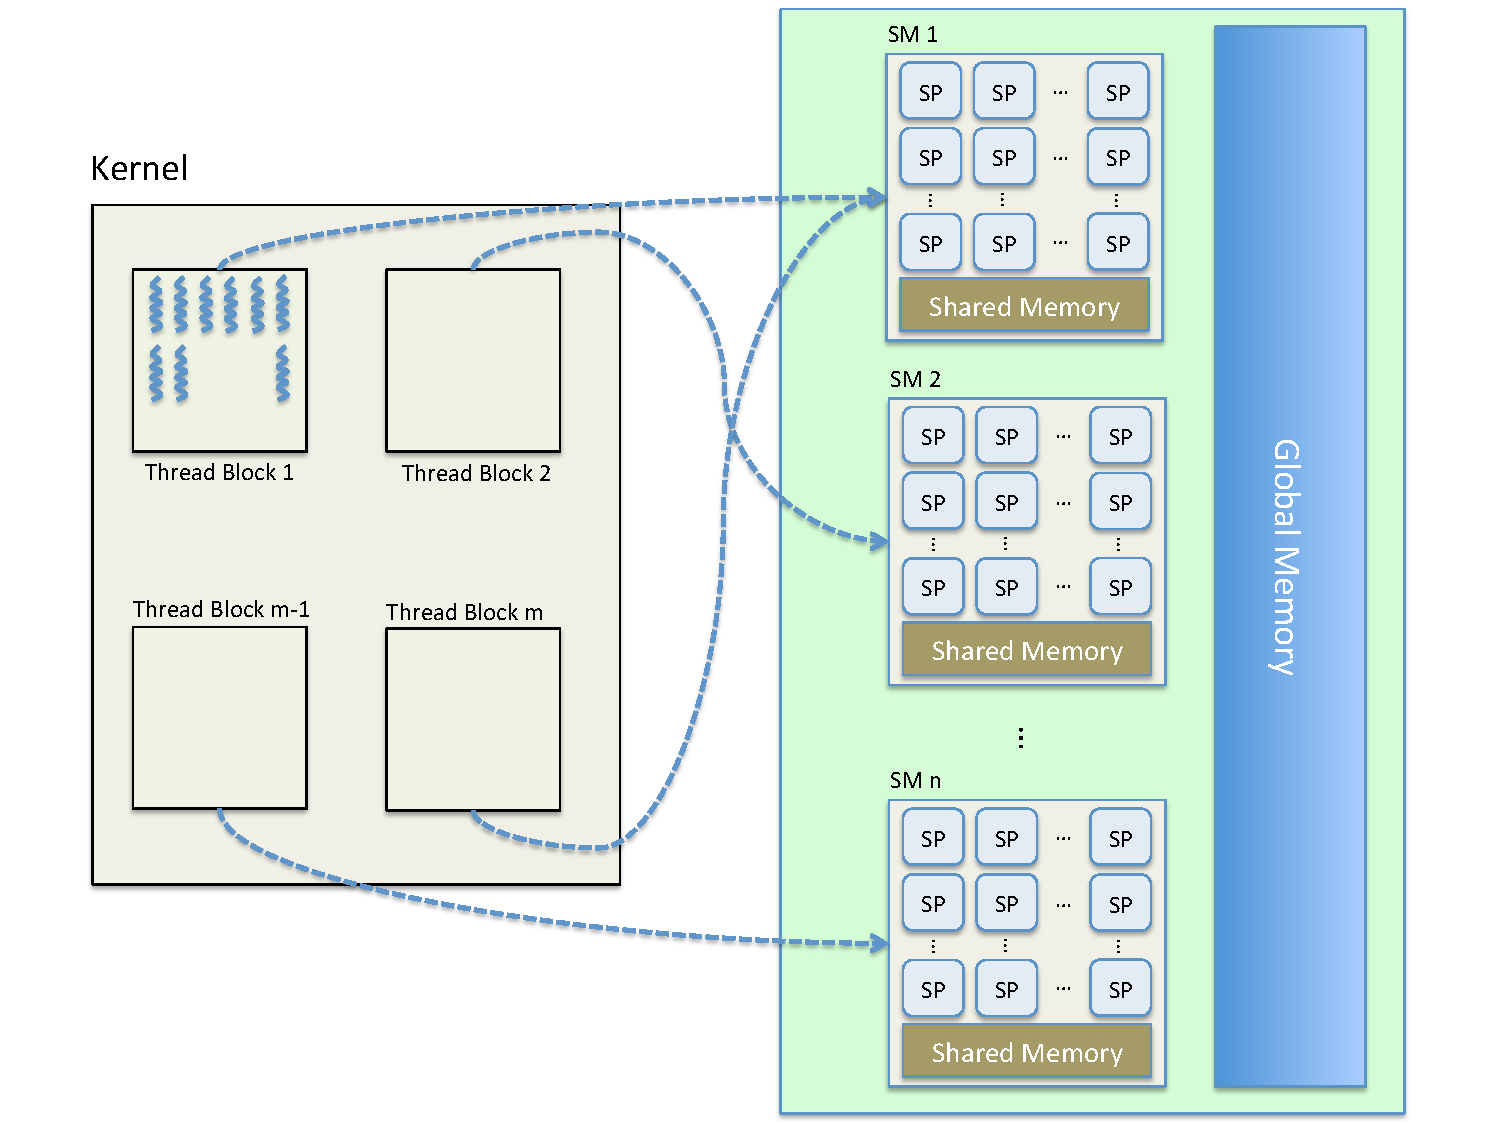
\includegraphics[width=0.9\linewidth]{figures/GPU-Kernel-Mapping.pdf}
\caption{Mapping of a GPU Kernel to the GPU device.}
\label{fig:GPU}
\end{center}
\end{figure}

The two most widely-used approaches to GPU programming, 
CUDA and OpenCL both aim to simplify the problem of programming GPUs, providing
similar portable, but low-level SIMD programming interfaces that can be executed on either CPUs or GPUs.
In each case, the basic unit of GPU computation is a \emph{kernel}, which
corresponds to a function that contains inherent data-parallelism, and which is
executed by each individual logical thread. Logical threads
are grouped into \emph{thread blocks}, which are mapped to
the symmetric multiprocessors (SMs) of the GPU (see Figure~\ref{fig:GPU}). 
Threads within one thread block are scheduled automatically on
their associated SM. Below is an example of a simple OpenCL kernel for adding two
vectors of real numbers:
\begin{lstlisting}
__kernel void vecAdd(  __global double *a,   
                        __global double *b,                       
                        __global double *c,                  
                        const unsigned int n)                    
{                                                               
     // get global thread id
     int id = get_global_id(0);                                  
     // make sure we do not go out of bounds                      
     if (id < n)                                                 
        c[id] = a[id] + b[id];                                  
}                                                               
\end{lstlisting}
When executing this kernel on a GPU, each GPU thread executes the kernel code independently. 
Different threads will get different ids assigned to them (variable \lstinline{id}), and will, therefore,
compute different elements of the output vector \lstinline{c}. 
% The programmer usually needs to manually decide on the appropriate
% number of threads and thread blocks for the kernel, and
% also to write tedious and often error-prone code to transfer the
% required data to and from the GPU. 

Unfortunately, \emph{programmability} is still generally lacking
with CUDA and OpenCL: having initially restructured (or written) the
program into a data-parallel form, suitable for SIMD execution,
the programmer then needs to take care of a number of very low-level programming
aspects, including the number of threads and thread blocks,  data transfers between CPUs and GPUs, scheduling of 
computations on the GPUs, division of the work between CPUs and GPUs etc.
For example, even the simple kernel above requires 100-150 lines of 
OpenCL code just for managing its execution on a GPU.
This requires the programmer to have a deep understanding not only of
the problem that is being solved, but also of the underlying hardware 
architecture.  This usually results in a solution that is heavily optimised
for a particular hardware system and which, therefore, lacks \emph{performance 
portability}. The GPU code is also often highly fragile and likely to be error-prone.

%Section~\ref{sec:relatedGPU} discusses other approaches to programming
%GPUs. 
The \Lapedo{} framework aims to overcome the deficiencies of
GPU programming models by
exploiting functional language features and principles to provide high-level
abstractions over different heterogeneous processor types, and a variety
of parallel structure.

\subsection{GPU Programming in Erlang}
\label{gpuerlang}
%\emph{Possibly coding examples here? KH}
%\emph{We need to explain spawn etc. and give an example. KH}

Erlang has no native support for GPU programming. However,
a library containing OpenCL bindings is available~\cite{erlangopencl}\footnote{Available to download at
  \url{https://github.com/tonyrog/cl}}, 
This provides an Erlang interface
to low-level OpenCL functions to set up GPU computations, transfer data
to/from the CPU, and launch GPU kernels
implemented in OpenCL plus basic marshalling
mechanisms between \emph{binary} data structures in Erlang and C arrays.
An example Erlang code that uses this library is given in ~\ref{sec:gpuCodeGen}. 
% which can be used by OpenCL. 
While enabling programmers to write their
code in Erlang, this library does not simplify GPU programming,
since the programmer is still required to write code that is equivalent 
to programming directly in OpenCL. In the \Lapedo{} framework, we build
on this library and automate the process of generating the bookkeeping
OpenCL code. 




\section{Refactoring Tool Support}
%\subsection{Refactoring Tool Support}
%\subsection{Traditional Refactoring Techniques}
% \subsection{Background - Traditional, functional langs.}
\emph{Refactoring} is the process of changing the internal structure of a
program, while preserving its (functional) behaviour. 
% Usually, this is done to improve the code structure, or to allow it to be
% modified in some specific way.
In contrast to general program transformations,
refactoring focuses on purely
structural changes rather than on changes to program functionality,
and is generally applied semi-automatically (i.e. under programmer
direction), rather than fully automatically.
This allows programmer knowledge about e.g. safety properties to be 
exploited, and so permits a wider range of possible transformation.
Refactoring has
many advantages over traditional transformation and fully automated approaches,
including (but not limited to):
\begin{itemize}
\item Refactoring is aimed at improving the design of software. As programmers
  change software to meet new requirements, so the code loses structure;
  regular refactoring helps tidy up the code to retain a good structure.
\item Refactoring makes software easier to understand. Programmers often
  write software without considering future developers. Refactoring
  can enable the code to better communicate its purpose.
\item Refactoring encourages code reuse by removing duplicated code~\cite{brownpepm}.
\item Refactoring helps the programmer to program faster and more effectively by encouraging
  good program design.
\item Refactoring helps the programmer to reduce bugs. As refactorings
  typically generate code automatically, it is
  easy to guarantee that this code is safe and correct~\cite{thompsonsultana}.
\end{itemize}

\noindent
The term ``refactoring'' was first introduced by Opdyke in his 1992 PhD
thesis~\cite{opdyke}, but the concept goes back at least to Darlington and
Burstall's 1977 \emph{fold/unfold} transformation system~\cite{darlington77},
which aimed to 
improve code maintainability by transforming Algol-style recursive loops into a
pattern-matching style commonly used today.
Historically, most refactoring was performed manually with the help of
text editor ``search and replace'' facilities.
However,  in the
last couple of decades, a diverse range of refactoring tools have become
available for various programming languages,
that aid the
programmer by offering a selection of automatic refactorings. 
% Since the first sucessful refactoring tool (the
% \emph{Refactoring Browser}~\cite{smalltalk} for Smalltalk),
% there has been a growing number of refactorings tools for a
% variety of different languages such as: Java, C, C++, C\#, Python and UML
% (32\!). 
For example, the most recent release of IntelliJ IDEA refactorer supports 35
distinct refactorings for Java~\cite{intellij}.
%Typical refactorings and their descriptions can be found in
%Table~\ref{tab:typ_refacs}.
Typical refactorings include \emph{variable renaming} (changes all instances
of a variable that are in scope to a new name), \emph{parameter adding} 
(introduces a new parameter to a function definition and updates all relevant
calls to that function with a placeholder), \emph{function extraction} (lifts
a selected block of code into its own function) and \emph{function inlining}.



% Typical refactorings include:
% \begin{itemize}
% \item Rename Variable/Function/Method
% \item Add Parameter
% \item Extract Function
% \item Inline Method
% \end{itemize}

%% VJ : I've commented this out. I think having infinitely many tables just makes
%%      things more complicated. I've inlined this into the text. If someone is
%%      against this, feel free to put the table back
%% \begin{figure}
%% \begin{tabular}{p{8em}p{25em}}
%% \hline
%% Refactoring & Description \\
%% \hline
%% Rename Variable & Changes all instances of a variable name to the name as
%%                   given by the programmer. Changes only relevant (i.e.\@ in
%%                   scope) instances of that variable. Checks whether given
%%                   variable name is valid and usable. \\
%% Add Parameter & Introduces a new parameter to a function definition; updates all
%%                 relevant calls to that function with a placeholder (possibly
%%                 as provided by the programmer). \\
%% Extract Function & Lifts a selected block of code into its own
%%                    function. Automatically determines and links required
%%                    parameters for the new function. Should the programmer
%%                    provide a name for the function, that name will be checked
%%                    for validity. \\
%% Inline Function & Removes a function, replacing all calls to it with said
%%                   function's body. \\
%% \hline
%% \end{tabular}
%% \caption{Common Refactorings}
%% \label{tab:typ_refacs}
%% \end{figure}


%% VJ: Move this to some Appendix
%\begin{figure}
%\begin{tabular}{>{\itshape}p{8em}p{25em}}
%\hline
%Refactoring & Description \\
%\hline
%% %ParMapIntroSeq & Introduces a map skeleton over a pre-existing func \\
% ParMapIntroSeq & Introduces a \verb+map+ skeleton over a pre-existing \verb+func+
%                  skeleton, given decomposition and recomposition functions. \\ 
% ParMapIntroComp & Transforms a list comprehension into a call to \emph{Skel}
%                   with a \verb+map+ skeleton, given decomposition and recomposition
%                   functions. \\
% FarmIntroSeq & Introduces a \verb+farm+ skeleton over a pre-existing \verb+func+ skeleton,
%               given a number of workers. \\
% FarmIntroMap & Transforms an Erlang map function into a call to \verb+Skel+ with
%              a \farm skeleton, given a number of workers. \\
%FarmIntroComp & Transforms a list comprehension into a call to \verb+Skel+ with
 %               a \farm skeleton, given a number of workers. \\
%FarmIntroComp2 & Extension of \verb+FarmIntroComp+, allowing nested function
%                 calls in the right hand side of the list comprehension. Nested
%                 function calls are converted into a \verb+farm+ skeleton with a
%                 nested parallel pipeline for each worker. \\
%IntroChunkComp & Transforms a list comprehension into a call to \verb+Skel+ with
%                 a \verb+map+ skeleton, given decomposition and recomposition
%                 functions. \\ 
%IntroChunkFarm & Transforms the \verb+farm+ skeleton in a call to \verb+Skel+ into a
%                 \verb+map+ skeleton, given decomposition and recomposition
%                 functions. \\
%\hline
%\end{tabular}
%\caption{Existing Refactorings Used}
%\label{tab:used_refacs}
%\end{figure}

%% VJ: Move this to where we discuss new stuff
%% \begin{figure}
%% \begin{tabular}{>{\itshape}p{10em}p{25em}}
%% \hline
%% Refactoring & Description \\
%% \hline
%% \multicolumn{2}{c}{\emph{Hybrid Skeleton Introductory Refactorings}} \\
%% \hline
%% HybFarmIntroSeq & \emph{insert def. here} \\
%% HybMapIntroSeq & \emph{insert def. here} \\
%% \hline
%% \multicolumn{2}{c}{\emph{Program Shaping Refactorings}} \\
%% \hline
%% ListToBinary & Transforms a set of recursive functions using one or more
%%                parameterised lists to an equivalent set of recursive functions
%%                using parameterised binaries. Updates functions and variables
%%                affected by this change to use the newly transformed binary
%%                functions. \\
%% List/BinaryToETS & Introduces an ETS table used to store inputs between
%%                    skeletons. Updates functions found within the call to
%%                    \emph{Skel} to store and extract from this table. \\
%% GPUWorkerGeneration & \emph{insert def. here} \\
%% \hline
%% \end{tabular}
%% \caption{Refactorings Introduced by Category}
%% \label{tab:introd_refacs}
%% \end{figure}


\subsection{Refactoring for Functional Languages}

Whilst the refactoring community has produced a great deal of work on
refactoring for the object-oriented paradigm~\cite{Dig}, the concept is
nevertheless applicable to a wide range of programming styles and
approaches. Functional programming is no exception to this. Indeed, Darlington
and Burstall's transformation system for recursive functions produces code that
would not be out of place in modern functional programs~\cite{darlington77}. The
University of Kent has since produced the HaRe~\cite{hare} and
Wrangler~\cite{wrangler} refactoring tools for Haskell and Erlang
respectively. Both tools are implemented in their respective languages, and
offer a number of standard refactorings . Wrangler is
implemented in Erlang and is integrated into both Emacs and Eclipse (Figure
\ref{wranglerscreenshot}). We exploit a recent Wrangler extension which
allows refactorings to be expressed as AST traversal strategies in terms of
their pre-conditions and transformation rules.  %The extension comes in two
%parts: a user-level language for describing the refactorings
%themselves~\cite{wranglerdsl2}; plus a Domain-Specific-Language to compose the
%refactorings~\cite{wranglerdsl}.




% The prototype
% refactorings presented in this paper have been implemented in the
% \textbf{Wrangler} refactoring tool \cite{wrangler}. %, the Erlang refactoring
% tool developed at the University of Kent by Li and Thompson.  Wrangler is
% implemented in Erlang and is integrated into both Emacs and Eclipse (Figure
% \ref{wranglerscreenshot}).  %% Unimportant detail? KH % Wrangler uses the Erlang
% \texttt{syntax\_tools} library in % order to obtain the necessary Abstract
% Syntax Trees (ASTs) which are then extended post-hoc with static semantic
% information (such as use and bind locations for variables).  %Figure
% \ref{wranglerscreenshot} shows a screenshot of Wrangler in AquaMacs (a typical
% Emacs environment for Mac OS X).  We exploit a recent Wrangler extension which
% allows refactorings to be expressed as AST traversal strategies in terms of
% their pre-conditions and transformation rules.  The extension comes in two
% parts: a user-level language for describing the refactorings
% themselves~\cite{wranglerdsl2}; plus a Domain-Specific-Language to compose the
% refactorings~\cite{wranglerdsl}.




% The refactorings are applied automatically to a selected piece of syntax in the refactoring editor
% and are fully implemented in the Wrangler~\cite{wrangler} refactoring
% tool for Erlang, as shown in  Figure \ref{wranglerscreenshot}.
% % \subsubsection{The Wrangler Refactoring Tool for Erlang.}
% % The prototype refactorings presented in this paper have been implemented in the  Wrangler refactoring tool \cite{wrangler}. %, the Erlang refactoring tool developed at the University of Kent by Li and Thompson.
% Wrangler itself is implemented in Erlang and is integrated into both Emacs and Eclipse.
% Figure~\ref{wranglerscreenshot} shows Wrangler in Emacs, presenting a menu of refactorings for the user.
% Like most interactive semi-automatic refactoring tools, 
% the user follows a number of steps in order to invoke a refactoring:
% \begin{enumerate}
% \item The user starts with either an Emacs or an Eclipse session, with their sequential or parallel code.
% \item The user identifies and highlights a portion of code that is amenable for refactoring in the text editor.
% \item The appropriate refactoring is then selected from the Wrangler drop down menu. This step requires user-knowledge.
% \item Wrangler will then ask the user for any additional parameters, such as the number of workers, any additional functions, or any additional information, such as new names for any new definitions that may be introduced by the refactoring process.
% \item Wrangler then checks the pre-conditions, and if the pre-conditions hold, the program is transformed by the tool, depending on the refactoring rule  being invoked.
% \item The source code in the editor is automatically changed to reflect the refactored program.
% \end{enumerate}

% The prototype refactorings presented in this paper have been implemented in the  \textbf{Wrangler} refactoring tool \cite{wrangler}. %, the Erlang refactoring tool developed at the University of Kent by Li and Thompson.
% Wrangler is implemented in Erlang and is integrated into both Emacs and Eclipse (Figure \ref{wranglerscreenshot}). 
% %% Unimportant detail? KH
% % Wrangler uses the Erlang \texttt{syntax\_tools} library in
% % order to obtain the necessary Abstract Syntax Trees (ASTs) which are then extended post-hoc with static semantic information (such as use and bind locations for variables).
% %Figure \ref{wranglerscreenshot} shows a screenshot of Wrangler in AquaMacs (a typical Emacs environment for Mac OS X).

\subsection{Refactoring for Parallelism Introduction and Tuning}

%\emph{This was horribly vague and imprecise. Needs to include other approaches, e.g. Danny Dig's Java one, SkePU...  We should probably include some examplesshowing what we are trying to do.  KH}

% Parallel refactoring is the process of introducing or tuning parallelism
% within programs via a refactoring tool. Similar to sequential refactoring,
% parallel refactoring relies on user knowledge in
% the sense that through the use of a refactoring tool, the user introduces
% and tunes parallelism in his/her applications.  
Some recent work has attempted to exploit refactoring technology to
introduce and tune parallelism.  For example, we have developed
prototype refactorings for parallel Haskell using the HaRe~\cite{hare} system,
and also extended Wrangler with a number of novel refactorings to
introduce and tune parallelism using skeletons via
the Skel library~\cite{hlpp}.  We have extended this work to
introduce and tune skeletons in C/C++~\cite{pdp2014}
using the FastFlow skeleton library, embedding our refactorings in the
Eclipse IDE.
%
In addition to the general advantages above, there are a number of specific advantages to using refactoring for parallelism
introduction and tuning:
% There are many advantages to parallel refactoring~\cite{ijpp}, some of which we state here (in addition to the advantages of general refactoring as given above):
\begin{itemize}
\item Using a refactoring tool to introduce skeletons (instead of
  manual insertion) means that the programmer has to understand and
  remember less. This enables them to concentrate more on the
  design of the program.
\item A refactoring tool can help minimise changes
 between different releases or implementations of skeletons.
\item \emph{By design}, a refactoring tool will not allow a user to break their
  programs. Introducing an incorrect skeleton, for example, is simply not
  allowed.
\end{itemize}

\noindent
These advantages are exploited by \Lapedo{} (described in more detail in Section~\ref{lapedoframe}).
In this paper, we will also take the concept of parallel refactoring further, however: by
introducing novel refactorings that introduce \emph{hybrid skeletons} for
heterogeneous systems, and by using refactoring for \emph{program
  shaping}.

\subsubsection{The PaRTE Refactoring Tool for Erlang.}
\label{parte}
The prototype refactorings presented in this paper have been implemented in the  \emph{Paraphrase Refactoring Tool for Erlang} (PaRTE). 
PaRTE integrates capabilities of the RefactorErl~\cite{splst11} and
Wrangler~\cite{wrangler} refactoring/program analysis tools into a new parallelisation
framework that can be used to identify parallel patterns
and determine the best implementations of those patterns~\cite{Bozo}. Both the
pattern candidate detection/assessment and semantics-preserving
transformation steps require thorough syntactic and semantic analysis.
This is achieved by exploiting the RefactorErl and Wrangler refactoring
tools, which implement specific compile-time analyses, and
support syntax-based transformations. RefactorErl implements a
wide range of static semantic analyses, including scope analysis of
various language entities, side-effect analysis and callee approximation
of dynamic function calls. Most of these (higher-level)
semantic analyses build on results from dataflow and type analyses.
Based on the information uncovered by the semantic analyses,
RefactorErl can determine non-trivial properties of code fragments.
In the integrated PaRTE framework, it is therefore used to perform
pattern discovery and evaluation. Conversely, Wrangler has a
mature user interface for performing simple code rewriting, which
makes it a good choice for a tool to carry out parallelisation transformations.
In the integrated PaRTE framework, Wrangler is responsible
for defining and executing shaping transformations, and
for turning sequential computations into instances of parallel algorithmic
skeletons.

% refactoring tool \cite{wrangler}. %, the Erlang refactoring tool developed at the University of Kent by Li and Thompson.
Wrangler itself is implemented in Erlang and is integrated into both Emacs and Eclipse.
Figure~\ref{wranglerscreenshot} shows Wrangler in Emacs, presenting a menu of refactorings for the user.
Like most interactive semi-automatic refactoring tools, 
the user follows a number of steps in order to invoke a refactoring:
\begin{enumerate}
\item The user starts with either an Emacs or an Eclipse session, with their sequential or parallel code.
\item The user identifies and highlights a portion of code that is amenable for refactoring in the text editor.
\item The appropriate refactoring is then selected from the Wrangler drop down menu. This step requires user-knowledge.
\item Wrangler will then ask the user for any additional parameters, such as the number of workers, any additional functions, or any additional information, such as new names for any new definitions that may be introduced by the refactoring process.
\item Wrangler then checks the pre-conditions, and if the pre-conditions hold, the program is transformed by the tool, depending on the refactoring rule  being invoked.
\item The source code in the editor is automatically changed to reflect the refactored program.
\end{enumerate}
This process is also described in~\cite{BDH+13}.

\section{The \Lapedo{} Framework} \label{lapedoframe}
\begin{figure}[t]
\begin{center}
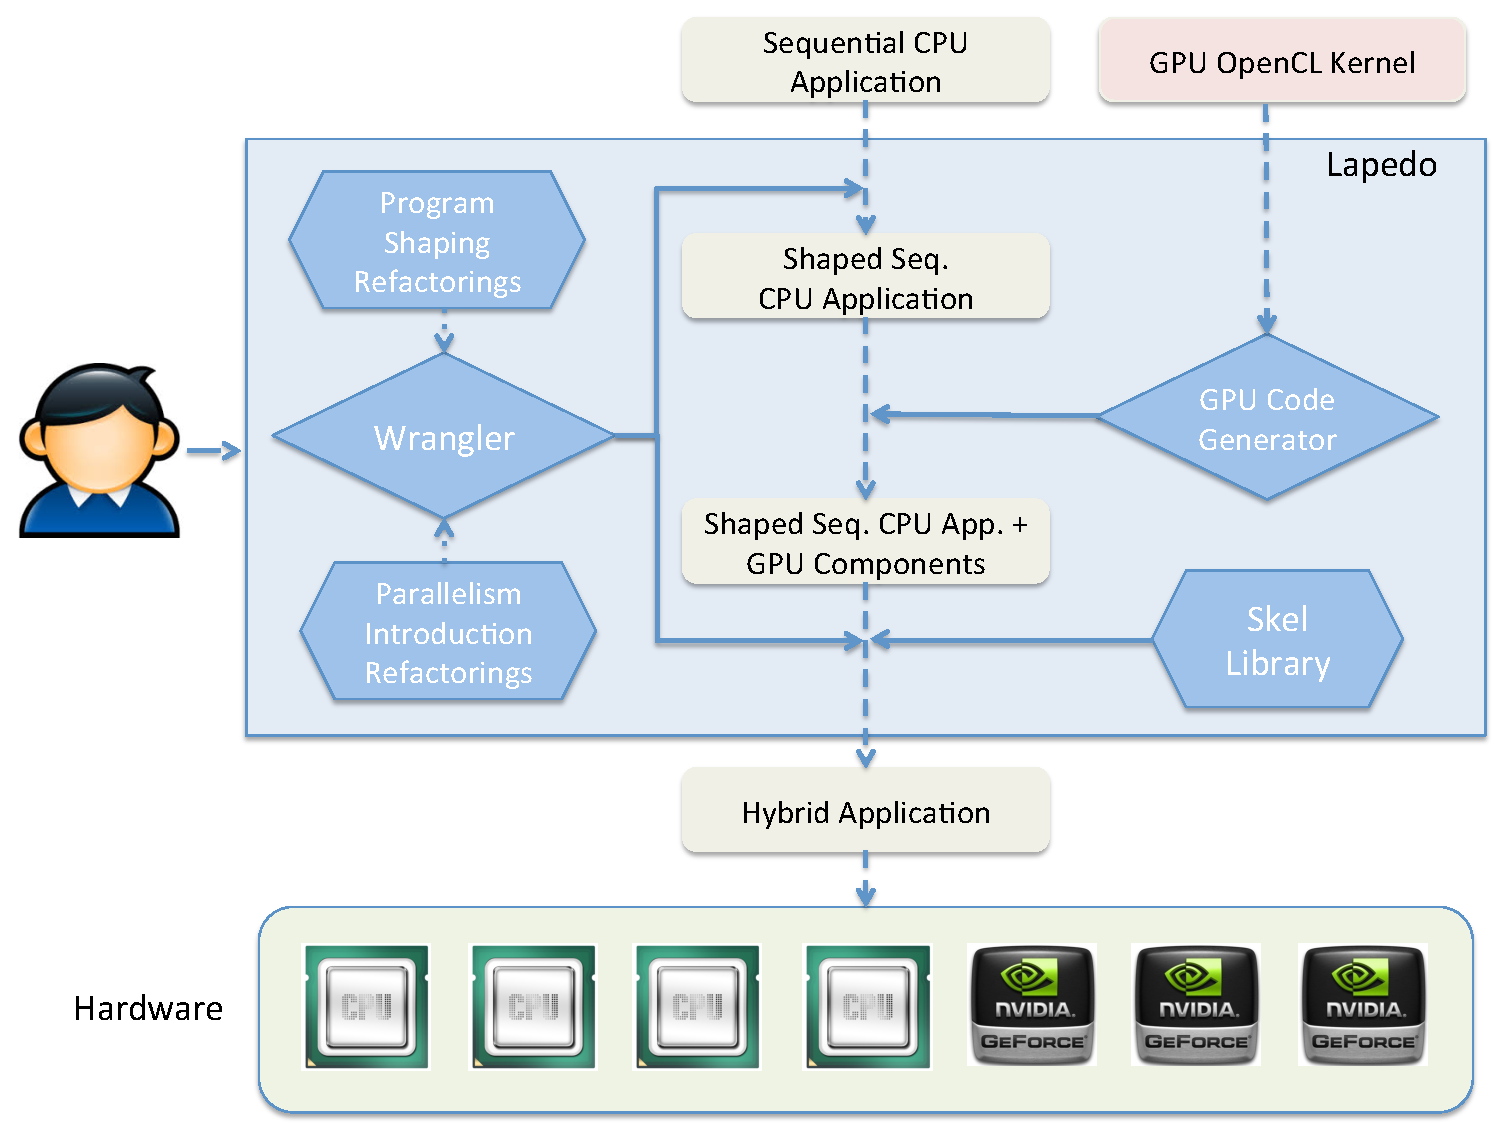
\includegraphics[width=0.9\linewidth]{figures/lapedo.pdf}
\caption{Overview of the process of parallelisation of Erlang programs
using \Lapedo.}
\label{fig:lapedoMethodology}
\end{center}
\end{figure}

\Lapedo{} aims to guide the programmer in the process of converting a
sequential or concurrent Erlang program into an equivalent parallel
version that can be executed efficiently on a heterogeneous multicore
system.  While \Lapedo{} primarily targets CPU+GPU combinations, it can
also, in principle, be used for other kinds of heterogeneous system that
support the OpenCL model (e.g.\ ones with FPGAs and/or Xeon Phis as well). \Lapedo{}
is built around the PaRTE refactoring tool (Section~\ref{parte}) and the \emph{Skel} 
library (Section~\ref{sec:skeletons}). Three main novelties that \Lapedo{} brings to these
tools, and which enable programming of heterogeneous machines, are: 
\begin{itemize} 
\item \emph{hybrid skeletons} that can have both CPU and GPU components 
(Section~\ref{sec:hybridSkeletons});
\item new refactorings for introduction of hybrid skeletons and program shaping
to convert the data into the format suitable for processing on GPUs 
(Section~\ref{sec:hybridRefactorings}); 
\item a \emph{GPU Code Generation} tool
that generates the code for GPU components of hybrid skeletons (Section~\ref{sec:gpuCodeGen}).
\end{itemize}
%% Covered above. KH
% The parallelism refactorings that \Lapedo{} introduces have
% two purposes: i) to prepare the code for the introduction of parallelism
% by transforming it into the right shape (\emph{program shaping}); and,
% ii) to introduce the parallel patterns into the sequential code
% (\emph{parallelism introduction}).
%
Figure~\ref{fig:lapedoMethodology} provides an overview of the process 
that is involved in transforming an existing Erlang application into a
parallel equivalent using \Lapedo{}. This method is described in the EU deliverable~\cite{transformationsystem} in more detail.
The programmer starts with a sequential (or concurrent) CPU application and an OpenCL kernel that
provides a GPU implementation for suitable operations in the application.
The programmer then performs the following steps (which may be  repeated if necessary):

\begin{enumerate}
\item \emph{Program shaping.}
The programmer first uses Wrangler to apply any necessary
program shaping transformations. 
For example, as described in Section~\ref{gpuerlang}, 
the basic Erlang OpenCL bindings only support the transfer of binary data 
to the GPU, so any data-structure that is to be used by the GPU kernel 
must be converted into binaries, together with the associated operations. These, and other 
program shaping transformations, are described in more detail in 
Section~\ref{sec:shaping}. This step is semi-automatic, requiring
the programmer to select the regions of the code that need to be
transformed, and to choose the appropriate transformations;
\item \emph{GPU code generation.} In the next step, the programmer invokes the 
\emph{GPU Code Generator} to generate Erlang code for the GPU components of the
future hybrid application. 
%  The programmer provides basic information about the available GPU kernels, and 
% he GPU Code Generator 
This generates code to link with and execute GPU kernels
(e.g.\ to manage data transfers to/from the GPU and to schedule the GPU 
computations),
based on programmer-supplied information about the kernels.
The GPU Code Generator is described in more detail in
Section~\ref{sec:gpuCodeGen}. This step is semi-automatic,
requiring the programmer to supply information about the GPU kernels;
\item \emph{Introduction of hybrid patterns.} Finally, the programmer uses
Wrangler again to refactor the shaped CPU code in order to introduce 
hybrid skeletons. This results in a hybrid application that uses the GPU components
that have been generated in the previous step. Hybrid skeletons are described in more
detail in Section~\ref{sec:hybridSkeletons}, and the refactoring that
introduce them are described in Section~\ref{sec:hybridRefactorings}. 
This step is semi-automatic, requiring the programmer to
select the regions of the code that can be parallelised using high-level
parallel patterns and to choose the appropriate hybrid pattern from the \emph{Skel} library.
\end{enumerate}

\noindent
We will use the parallelisation of an \emph{N-Body Simulation} to
illustrate how the \Lapedo{} framework can be used in practice.
This application is a simulation of
a dynamic system of particles under the influence of external forces. It
is commonly used in astronomy, for example, to simulate movements of the
planets.  The simulation proceeds in a number of iterations, each of
which computes a new position for each particle, based on its
interactions with all the other particles in the system. The core of the
application is the \lstinline{nbody} function:

%\hrules
\begin{lstlisting}
nbody(Parts,Dt,0) -> Parts;
nbody(Parts, Dt, NrIters) ->
  NewParts = lists:map (fun(X) -> nbody_one_part_cpu (X,Parts,Dt) end, Parts),
  nbody(NewParts, Dt, NrIters-1).
\end{lstlisting}
%\hrulee

\noindent
This function applies the \lstinline{nbody_one_part_cpu} function to each
element of the input list of particles, \lstinline{Part}. \lstinline{Dt}
is a constant that is passed to the \lstinline{nbody_one_part_cpu}
function. The \lstinline{nbody_one_part_cpu} function is given below:

%\hrules
\begin{lstlisting}
nbody_one_part_cpu(Part, Particles,Dt) ->
    {Ax,Ay,Az} = calc_acc_vector_list (Part, Particles),
    {X,Y,Z,M,Vx,Vy,Vz,_} = Part,
    Xnew = X + Dt*Vx + 0.5*Dt*Dt*Ax,
    Ynew = Y + Dt*Vy + 0.5*Dt*Dt*Ay,
    Znew = Z + Dt*Vz + 0.5*Dt*Dt*Az,
    Vxnew = Vx + Dt*Ax,
    Vynew = Vy + Dt*Ay,
    Vznew = Vz + Dt*Az,
    {Xnew,Ynew,Znew,M,Vxnew,Vynew,Vznew,0}.
\end{lstlisting}
%\hrulee

\noindent
The auxiliary \lstinline{calc_acc_vector_list} function is a simple fold
over the list of particles: 
%\hrules

\begin{lstlisting}
calc_acc_vector_list (Part,Particles) ->
    lists:foldl(fun(X,Sum) -> add_to_acc_list(X,Sum,Part) end,
                 {0,0,0}, Particles).
\end{lstlisting}
%\hrulee

\noindent
We omit the definition of the \lstinline{add_to_acc_list} function. We
also assume that we have available an OpenCL kernel
\lstinline{nbodyKernel} that applies the \lstinline{nbdoy_one_part_cpu}
function to a chunk of particles.
%
We can see that the main part of the code (in the \lstinline{nbody}
function) involves applying the same function to a list of particles.
This suggests that it can be parallelised by using a \lstinline{farm} or
\lstinline{cluster} skeleton. Since 
each individual computation on particles is relatively small but the total
number of particles involved is potentially large,
we have chosen to use a
\lstinline{chunking} pattern (so as to group particles into coarse-grained chunks that
will be processed sequentially by worker processes), and use \Lapedo{} for
parallelisation as follows:
\begin{enumerate}
\item We first need to perform some \emph{program shaping} transformations
  in order to prepare the code for the introduction of the \emph{chunking} pattern. 
  Since the idea is to split the initial list of particles into a list of lists (chunks) and then
  apply sequentially the \lstinline{nbody_one_part_cpu} function to these chunks,
   \lstinline{nbody_one_part_cpu} will need to be applied to chunks of particles, 
   rather than to just the individual particles. However, since we have a GPU kernel that
  calculates \lstinline{nbody_one_part_cpu} for a chunk of particles,
  and since GPU kernels can only operate on binary data, our instance of the
  \lstinline{chunk} skeleton needs to work on binaries rather than with
  lists. We, therefore, apply the \emph{ListChunking} and
  \emph{ListToBinary} program shaping refactorings from Section~\ref{sec:shaping} to modify the
  \lstinline{nbody_one_part_cpu} to: i) operate on chunks of particles; and
  ii) operate on binary data.
% , by allowing it to accept binary argument
%   and converting all list operations into equivalent operations with
%   binaries.  
  Since Erlang binaries are essentially just streams of bytes, we
  need to specify the size (in bytes) of each data item (particle in our
  case), so that we can correctly apply the binary \emph{map} and \emph{fold}
  functions. 
%  \emph{Duplicate name here! KH}
  The resulting code introduces the
  \lstinline{nbody_chunk_cpu} function to apply
  \lstinline{nbody_one_part_cpu} over individual chunks of the input data:

%\hrules
\begin{lstlisting}
nbody_chunk_cpu(Chunk, Particles,Dt) ->
  binary8Map(fun nbody_one_part_cpu/3, Chunk).
\end{lstlisting}
%\hrulee

\noindent
%\emph{This seems incredibly specific -- you need to explain how to
%  generalise it, e.g. by generating a family of functions!  KH} \emph{Yeah, that's the point, since this is an example. VJ} \emph{Needs to talk about binary data rather than binaries, and/or explain this earlier in the Erlang section.}
The \lstinline{binary8Map} function maps over a
binary object where each data item is precisely 8 bytes long.  Since it
contains no explicit operations over binaries, the body of the
\lstinline{nbody_one_part_cpu} function remains unchanged. However,
the \lstinline{calc_acc_vector_list} must be changed to use a binary fold
rather than the original list version:

%\hrules
\begin{lstlisting}
calc_acc_vector_list (Part,Particles) ->
    binary8Foldl(fun(X,Sum) -> add_to_acc_list(X,Sum,Part) end, 
                 {0,0,0}, Particles).
\end{lstlisting}
%\hrulee

\noindent
As with \lstinline{binary8Map}, \lstinline{binary8Foldl} operates over
8-byte wide binary data.

\item We can then invoke the GPU Code Generator to generate a wrapper around
  the GPU kernel, creating a GPU component, \lstinline{nbody_chunk_gpu},
  whose functionality is identical to that of
  \lstinline{nbody_chunk_cpu}. Certain parameters, such as
  \lstinline{K#kwork.localSize} and \lstinline{K#kwork.globalSize}, cannot
  be automatically generated at present, however, and therefore
  need to be supplied by the programmer.  The
 generated code is shown below:

%\hrules
\begin{lstlisting}
nbody_chunk_gpu(Chunk, Particles, Dt)	 ->
    %% set up the environment
    E = clu:setup(all),
    {ok,Program} = clu:build_source(E, program(ok)),
    {ok,Kernel} = cl:create_kernel(Program, "nbodyKernel"),
    
    ...

    %% create buffers
    {ok,ChunkInBuffer} = cl:create_buffer(E#cl.context,[read_only],
                                          byte_size(Chunk)),
    {ok,ParticlesBuffer} = cl:create_buffer(E#cl.context,[read_only],
                                            byte_size(Particles)),
    {ok,ChunkOutBuffer}  = cl:create_buffer(E#cl.context,[read_only],
                                            byte_size(Chunk)),

    ...

    %% data transfers
    {ok,E1} = cl:enqueue_write_buffer(K#kwork.queue,
                                      ChunkInBuffer,
                                      0, byte_size(Chunk),
                                      Chunk, []),
    {ok,E2} = cl:enqueue_write_buffer(K#kwork.queue,
                                      ParticlesInBuffer,
                                      0, byte_size(Particles),
                                      Particles, []),

    ...
                                   
    %% Set kernel arguments
    ok = cl:set_kernel_arg(Kernel, 0, ChunkInBuffer),
    ok = cl:set_kernel_arg(Kernel, 1, ParticlesInBuffer),
    
    ...

    %% enqueue the kernel
    Global = K#kwork.globalSize,
    Local = K#kwork.localSize,
    {ok,E6} = cl:enqueue_nd_range_kernel(K#kwork.queue,
                                        Kernel,
                                        [Global], [Local],
                                        [E1,E2]),

    ...

    %% read back from the GPU
    {ok,E7} = cl:enqueue_read_buffer(K#kwork.queue,
                                    ChunkOutBuffer,
                                    0, byte_size(Chunk), [E6]),
    Result = case cl:wait(E7,3000) of
             {ok, Data} ->
                  Data;
             Res3 ->
                  Res3
             end,

    ...

    %% return the result
    Result.
\end{lstlisting}
%\hrulee

\item Finally, since we now have the CPU and GPU components
  (\lstinline{nbody_chunk_cpu}) and \lstinline{nbody_chunk_gpu}),
  and both 
  operate over binary chunks, we can introduce the \emph{cluster} skeleton. We apply the \emph{IntroduceHybridCluster} refactoring
  from Section~\ref{sec:hybridRefactorings} to obtain the following parallel version of the
  main function. % , \lstinline{nbody}:

%\hrules
\begin{lstlisting}
Struct = {hyb_cluster, [{hyb_map, [{func, fun(X) ->
 nbody_cpu:nbody_cpu(X,Particles,Dt) end}], 
                           [{func, fun(X) ->
                            nbody_gpu:nbody_gpu(X, Particles, Dt) end}]}],
              TimeRatio, fun struct_size/1, fun make_chunk/2, 
              fun lists:flatten/1,
              NrCPUWs, NrGPUWs},
Res = skel:do([Struct],[Particles]).
\end{lstlisting}
%\hrulee

%\noindent
 % This must then be applied to the stream of input data to obtain the final
 % skeletal program.

%\noindent
%\hrules
%\begin{lstlisting}
%...
%\end{lstlisting}
%\hrulee
\end{enumerate}

%In the next sections, we describe components of the \Lapedo{} framework. In
%Section~\ref{sec:hybridSkeletons} we describe extension to the Skel library
%that allows combining CPU and GPU components within the same skeleton. In
%Section~\ref{lapedo-refactorings} we describe new refactorings to introduce
%hybrid skeletons and to shape the application so that GPU components can be
%introduced. In Section~\ref{sec:gpuCodeGen} we describe a command-line tool
%to generate the code for GPU components. Finally, in %Section~\ref{sec:workDiv}
%we describe how the work is divided between CPU cores and GPUs.


%% Cut for now - I think we may have enough upfront.  KH
% \section{Erlang}

\subsection{Hybrid Skeletons in Lapedo}
\label{sec:hybridSkeletons}

Hybrid skeletons that Lapedo provides were described in detail in~\cite{parco2015}. Here, we just give a brief overview of them, relevant to the refactorings presented in Sections~\ref{lapedo-refactorings}. The skeletons provided are:

\begin{itemize}
\item \emph{Hybrid Farm} represents a hybrid variant of a \emph{farm} skeleton, where the same operation is applied to a set of independent input values. The hybrid variant has different implementations of the operation for each of the different types of processors in the system. Currently, CPUs and GPUs are supported as the processor types. We support either explicit or implicit distribution of work between different kinds of workers, as described in~\cite{parco2015}. The syntax of the hybrid farm skeleton is

\begin{lstlisting}
{hyb_farm, CPUWorkflow, GPUWorkflow, [NCPUWorkers, NGPUWorkers]}
\end{lstlisting}

\noindent
where \lstinline{CPUWorkflow} and \lstinline{GPUWorkflow} represent CPU and GPU implementations of the farm operation, and optional parameters \lstinline{NCPUWorkers} and \lstinline{NGPUWorkers} denote the number of CPU and GPU workers, in the case that the work needs to be explicitly divided between the two worflows (using \lstinline{NCPUWorkers}:\lstinline{NGPUWorkers} ratio between work executed on CPU and GPU).

%The hybrid farm skeleton, \lstinline{hyb_farm}, requires two
%inner workflows: one for a CPU and another for a GPU.
%%Before the elements of the input stream are sent to the
%inner workflows, they need to be tagged with either a \texttt{cpu}
%or a \texttt{gpu} tag, which mark the element for
%processing by the CPU or the GPU workflow, respectively.
%In the future, additional tags will be suported to accommodate for
%additional accelerator types. Depending on whether the tagging
%of the input elements is done outside of the hybrid map (e.g.~by some
%outer workflow) or by the hybrid map skeleton itself. 
%There are two flavours of \lstinline{hyb_farm}:

%\begin{itemize}
%\item \lstinline|{hyb_farm, CPUWorkflow, GPUWorkflow}|, where the tasks in %the input stream
%  that are passed to the skeleton are already tagged;
%\item \lstinline|{hyb_farm, CPUWorkflow, GPUWorkflow, NCPUWorkers, NGPUWorkers}|,
%  which accepts any input stream and tags each task before sending the task to
%  one of the two worflows. The \texttt{NCPUWorkers} and \texttt{NGPUWorkers}
%  parameters are used to determine the ratio of tasks that are tagged with these
%  two tasks.
%\end{itemize}
%As an example, \lstinline|{hyb_farm, {func, fun f_CPU}, {func, fun f_GPU}, 4, 1}|
%denotes a hybrid map where elements of an input stream are sent for processing
%to either the \lstinline|f_CPU| or \lstinline|f_GPU| function. Tagging of the
%elements of the input stream is done by the skeleton itself, and in this case, four times more
%elements will be tagged with the \texttt{cpu} tag than with the \lstinline{gpu} tag.

\item \emph{Hybrid Cluster} skeleton accepts an input stream
of tasks, decomposes each task into chunks of subtasks and passes them to one of the two inner workflows (CPU or GPU workflow, similar as in the hybrid farm skeleton). There are several different variants of the \lstinline{hyb_cluster}
skeleton, differing in whether the programmer provides the decomposition 
and recomposition functions, otherwise these are automatically provided by the library. In the paper, we consider two versions:
\begin{itemize}
\item \lstinline|{hyb_cluster, CPUfl, GPUfl, MinChSz, Ratio, NCPUW, NGPUW}|,
where each element of an input stream is a list and \lstinline{CPUfl} and 
\lstinline{GPUfl} are CPU and GPU workflows that process list chunks (sublists).
\lstinline{MinChSz} is the minimum size of a list chunk, which can be chosen so that
the \lstinline{GPUfl} executed on a chunk of that size gives the maximum parallelism
(e.g.~\lstinline{MinChSz} can be chosen to be a maximum number of list items that
the GPU can process at the same time). \lstinline{Ratio} is the ratio between the time it
takes to process a chunk of \lstinline{MinChSz} using \lstinline{CPUfl} and 
\lstinline{GPUfl}, and \lstinline{NCPUW} and \lstinline{NGPUW} are number of processes
executing \lstinline{CPUfl} and \lstinline{GPUfl} workflows. In the case where there
is no nesting, i.e.~where \lstinline{hyb_cluster} is the top-level skeleton and 
\lstinline{CPUfl} and \lstinline{GPUfl} are \lstinline{func} skeletons, \lstinline{NCPUW}
and \lstinline{NGPUW} should be set to the number of CPU cores and the number of physical GPU
devices available in the system, respectively.

\item \lstinline|{hyb_cluster, CPUfl, GPUfl, Ratio, SzFun, MkChFun, RecompFun}|, where
 \lstinline{CPUfl}, \lstinline{GPUfl} and \lstinline{Ratio} are in the version above.
This version does not assume that the elements of an input stream are lists. Here, programmer
provides functions for determining the size of an element (\lstinline{SzFun}), creating a
chunk of work with a specified size from an element of an input stream 
(\lstinline{MkChFun}) and recomposing a list of chunks into
a data structure of the output element (\lstinline{RecompFun}). This skeleton uses a generic
decomposition function, that successively calls \lstinline{MkChFun} to decompose an
element of an input stream into a list of chunks, tagging them in the process and passing them
to the inner workflows.
\end{itemize}
\end{itemize}

%Both versions of the hybrid cluster skeleton automatically calculate the sizes of the chunks into
%which an element of an input stream is decomposed, based on the %\lstinline{Ratio} parameter and
%the size of the element (calculated by either list length or %\lstinline{SizeFun} function). 
%This means that the chunk sizes are not equal -- depending on whether the GPU or the CPU workflow
%is faster in processing work, more work will be allocated to a GPU than to each CPU core (or vice
%versa). This allows the skeleton to adapt to the given workload and calculate a near-optimal 
%division of work between the CPU cores and the GPU. For more details on how %this is calculated,
%see Section~\ref{sect:workDiv}.

%There are several more versions of the \lstinline{hyb_cluster} skeleton. Some of them allow 
%automatic calculation of the \lstinline{Ratio} parameter by supplying a sampling chunk to 
%the skeleton, which then does profiling on this chunk using the CPU and the GPU workflow and
%calculates the ratio. Details about these additional hybrid cluster versions %can be found on 
%\url{http://blah.com}. We now give a few examples of the use of hybrid cluster skeleton.
%\begin{enumerate}
%\item \lstinline|{hyb_cluster, {func, fun f_CPU/1}, {func, fun f_GPU/1}, 64, 7, 5, 1}| denotes the
%  hybrid cluster skeleton that operates on a list of lists, with the \lstinline{f_CPU} and \lstinline{f_GPU} functions
%  processing sublists on CPU cores and GPUs, respectivelly. Each chunk
%  has a length that is a multiple of 64, and there are 5 workers that are bound to CPU cores, and 1 worker
%  that executes work on a GPU. In this case, we have calculated that the \lstinline{f_GPU} is 7
%times faster in processing sublists of length 64 than the \lstinline{f_CPU}. 
%\item In the NBody example described in Section~\ref{sect:}, after transformation,
 % input stream is a list of binaries. Each binary represent a set of particles, and each particle
 % is represented by 64 bytes of a stream. Furthermore, 
 % we have \lstinline{nbody_CPU(Chunk,Parts,Dt)} and \lstinline{nbody_GPU(Chunk,Parts,Dt)}
 % functions that process chunks of particles. In order to use the hybrid cluster skeleton, we need
 % to provide several auxiliary functions. Firstly, we need to provide the function to calculate the ``size''
 % of a binary, which will be used when decomposing a binary of particles. Since the basic unit for NBody computation
 % is a particle, which takes 64 bytes, the size of the binary will be the number of particles in it:

 % \begin{lstlisting}
 % struct_size(Binary) -> byte_size(Binary) div 64.  
 % \end{lstlisting}

 % Next, we need a function to build chunks of specific size (in terms of a number of particles in it).
 % This function takes a binary and a chunk size, and returns the
 % binary chunk and the rest of the original binary.

 % \begin{lstlisting}
 %   make_chunk(Binary, Size) ->
 %   {binary:part(Binary, {0,64*Size}),
 %    binary_part(Binary, {64*Size,byte_size(Binary)-64*Size})}
  %\end{lstlisting}

 % Finally, we need a function to take a list of binaries that are returned by \lstinline{nbody_CPU}
 % and \lstinline{nbody_GPU} and recompose them into a new binary with new coordinates of particles:

  %\begin{lstlisting}
   % flattenBinary(ListOfBinaries) ->
    %lists:foldl(fun (Binary, Acc) -> <<Acc,Binary>> end, 
   %             <<>>, ListOfBinaries).
  %\end{lstlisting}

 % If, for example, the best parallelism on a GPU is obtained when processing a chunk of 100 particles,
 % and if processing chunk of that size is 50 times faster on a GPU than on a CPU, then
 % we can build the following hybrid cluster skeleton:

  %\begin{lstlisting}
   % Cluster = {hyb_cluster, 
    %             {func, fun nbody_cpu/1}, 
     %%           100, 
       %          50,
        %         fun struct_size/1, 
         %        fun make_chunk/2, 
          %       fun flatten_binary/1,
           %      5, 
            %     1}.
  %\end{lstlisting}

  
  
%\end{enumerate}

%\subsection{Hybrid Farm.} %A task farm creates a number of worker 
%processes, executing in parallel on a stream
%of input tasks.
%The hybrid task farm skeleton, \lstinline{hyb_farm}, is similar to \lstinline{hyb_map},
%except that it does not require a splitting function: we assume
%that its input is a stream of already constructed
%tasks.

%\hrules
%\begin{lstlisting}
%hyb_farm = fun(NrCPUWs, NrGPUWs, CPU_W, GPU_W) ->
%            {farm, [{seq, fun(X) -> hyb_farm:hyb_dispatcher(CPU_W, GPU_W, X)
%                      end}], NrCPUWs+NrGPUWs}.
%\end{lstlisting}
%\hrulee

%\noindent
%Before calling the \lstinline{hyb_farm} skeleton, we need to tag the tasks
%in the input stream, similar to with \lstinline{hyb_map}:

%\hrules
%\begin{lstlisting}
%runFarm = fun(NCPUWs,NGPUWs) ->
%  ListOfTasks = <construct a list of tasks>,
%  TaggedList = tag_list (ListOfTasks, NCPUWs, NGPUWs),
%  skel:do {hyb_farm(NCPUWs, NGPUWs, fun cpu_w/1, fun gpu_w/1), TaggedList}.
%\end{lstlisting}
%\hrulee

%\noindent
%As with \lstinline{hyb_map}, \lstinline{hyb_farm:hyb_dispatcher} will schedule
%tasks as appropriate on the available CPU/GPU workers.

%\subsection{Work Division for Hybrid Skeletons}
%\label{sect:workDiv}

%\noindent
%The \lstinline{hyb_farm} and \lstinline{hyb_cluster} skeletons require the number 
%of CPU and GPU workers to be specified explicitly.
%In the cases where there is
%no nesting of skeletons, i.e.~where there is only a \lstinline{hyb_farm} or
%\lstinline{hyb_cluster} skeleton at the top level, and the inner skeletons are
%instances of \lstinline{func}, we can simply set the number of CPU workers to be
%equal to the number of cores in a CPU, and the number of GPU workers to
%be the number of physical GPU devices in the system. The problem with this,
%however, is that for suitable problems, GPUs are much faster in processing
%work than CPU cores. \lstinline{farm} and \lstinline{cluster} 
%skeletons (and, consequently, \lstinline{hyb_farm} and %\lstinline{hyb_cluster})
%use \emph{push} approach, where tasks are pushed in round-robin fashion 
%to the workers. Therefore, in the case of \lstinline{farm} and \lstinline{hyb_farm}
%skeletons, the same amount of work is assigned to each worker. This is also
%the case for \lstinline{cluster} and \lstinline{hyb_cluster} skeletons, if we use a
%simple splitting function that divides an input list into equally-sized 
%chunks. If GPUs can process tasks much faster, equal division of work is
%obviously a problem, since GPUs will finish much faster than CPU cores and will,
%therefore, have to wait until CPU cores finish their portion of work. 

%In the case of \lstinline{cluster}, the aforementioned problem can be avoided if we do 
%a smarter division of input lists into chunks. Assuming that a given problem is
%regular (i.e.~that it takes the same amount of time to process each element of
%an input data structure) and that we can obtain timing information (e.g.~using profiling)
%that can tell us how faster can a GPU process one list item (or a set of list items)
%than a CPU core, we can, using some simple formulas, derive how many
%list items should be processed by the GPUs and how much by each CPU core in order to
%get the best execution time. For example, assume that we have $g$ GPU and $c$ CPU cores
%in a system, and that the ratio between processing time for $k$ items between a CPU
%and a GPU is $\mbox{ratio}$. If an input list has $n$ items (where $n$ is divisible by
%$k$), then we can estimate the time it takes to process all of the items in the list if 
%$n_c$ items are processed
%by CPU cores by
%$$T(n_c) = \max \left \{ \left \lceil \frac{\frac{n_C}{k} \cdot \mbox{ratio}}{c} \right \rceil, 
%\left \lceil \frac{\frac{n-n_c}{k}}{g} \right \rceil \right \},$$
%where the first argument of the $\max$ is the time it takes to process $n_C$ items
%on CPU cores, and the second argument is the time it takes to process the remaining 
%items by the GPUs. The best time we can obtain is then $\min\{T(n_C) | n_C \in \{0,k,2k,...,n\}\}$,
%and the optimal number of items to process on CPU cores is such $n_C$ for which this
%minimum is obtained. In this way, we calculate a pair $(n_C,n-n_C)$, the number of
%list items to be processed by CPU cores and the GPUs, respectivelly. Chunk sizes for
%CPU cores are then 
%$$\left \{ \underbrace{\left \lfloor \frac{n_C}{c} \right \rfloor, \left \lfloor \frac{n_C}{c} \right \rfloor, \dots
%\left \lfloor \frac{n_C}{c} \right \rfloor}_{c - (n_c \; \text{mod} \; c) \; \text{times}}, \underbrace{\left \lceil \frac{n_C}{c} \right \rceil, \left \lceil \frac{n_C}{c} \right \rceil,
%\dots, \left \lceil \frac{n_C}{c} \right \rceil}_{n_c \; \text{mod} \; c \; \text{times}} \right \}.$$
%We can similarly calcuate the chunk sizes for the GPUs. The parameter $k$ in the above discussion
%should be chosen so that it gives the best parallelism on the GPU, i.e.~it should be maximum
%number of list items that the GPU can process in parallel (see Section~\ref{sec:eval} for
%examples). 

%For \lstinline{farm} skeleton, we can, if we know the length of the stream of tasks,
%calculate how many tasks should be evaluated by CPU cores and how much by the GPUs
%using a similar approach to above. Additionally, \lstinline{farm} can be implemented
%using the \emph{pull} (\emph{work stealing}~\cite{ws}) approach, so that the tasks are sent
%to the workers \emph{on-demand} when they request them, as oposed to eagerly in the
%\emph{push} approach. However, this method requires more communication, as the workers
%need to send messages to the emitter to request more work. It is, however, the preferred
%solution when tasks are irregular (i.e.~when some tasks are more computationally-intensive
%than others). Since the examples that we consider in this paper are regular, we do not
%use the work-stealing approach.

%In the case where there is a nesting of skeletons (e.g.~farm inside of a hybrid cluster), we cannot
%simply let all farms use all CPU cores and GPUs, since that would result in overloading
%the system with processes. For complex nestings of skeletons, it is highly non-trivial
%to derive the ``correct'' number of CPU and GPU workers for all farms/maps.
%In~\cite{cec}, we have described one method for that, based
%on Monte-Carlo Tree Search (MCTS) method.
%We plan to integrate this into \Lapedo{} in future.

\section{\Lapedo{} Refactorings for Hybrid Skeletons and Program Shaping}
\label{lapedo-refactorings}

%This section describes the new \Lapedo{} refactorings
%for introducing hybrid skeletons and for program shaping.
 %The refactorings themselves are divided up into three groups.
%In Section~\ref{sect:progshaping}, we give a number of refactorings for \emph{Program Shaping},
%which allows the programmer  
%\subsection{Rewrite Rules}
%


%\subsection{Refactoring Notation}

% Each refactoring that we will use in this paper will be described as a semi-formal transformation rule, with associated
% pre-conditions, operating over the abstract syntax tree (AST)
% of the source program. %, as a function that is applied
% %to a node of the AST and corresponds to traversals of the AST.
% %  (rules are generally top-down, unless otherwise stated; if a rule fails on an AST node, lower nodes are then examined).
% %We define our refactoring function:
% %\begin{small}
% %\begin{align*}
% % \vspace{-6pt}
% % \begin{small}
% $$\mathit{Refactoring(x_0,\ldots,x_n)} =  \ \{\mathit{Rule} \times \{\mathit{Condition}\}\}$$
% % \end{small}
% %\end{align*}
% %\end{small}
% % \noindent
% where $\mathit{Rule}$ is the transformation, $\{ \mathit{Condition} \}$ is the set of associated pre-conditions and  $x_0,..,x_n$ are the arguments to the refactoring. The
% refactoring rules are defined as functions over nodes that represent expressions in the AST:

% \vspace{-6pt}
% %\begin{small}
% %\begin{align*}
% %$$\mathcal{D} \llbracket . \rrbracket : \mathit{Declaration} \rightarrow \mathit{Declaration}$$
% %\begin{small}
% % $$\mathcal{M} \llbracket . \rrbracket : \mathit{Module} \rightarrow \mathit{Module}$$
% % $$\mathcal{D} \llbracket . \rrbracket : \mathit{Declaration} \rightarrow \mathit{Declaration}$$
% % $$\mathcal{E} \llbracket . \rrbracket : \mathit{Expr} \rightarrow \mathit{Expr}$$
% $$\mathcal{M} \llbracket . \rrbracket : \mathit{Module} \rightarrow \mathit{Module}$$
% $$\mathcal{D} \llbracket . \rrbracket : \mathit{Declaration} \rightarrow \mathit{Declaration}$$
% $$\mathcal{E} \llbracket . \rrbracket : \mathit{Expr} \rightarrow \mathit{Expr}$$
% %\end{small}
% %\end{align*}
% %\end{small}
% %
% %\vspace{-18pt}
% %\noindent
% %
% % \hspace*{-0.5ex}
% %Each rewrite rule has its own set of conditions which are enclosed by $\{ \}$.
% \noindent
% Choice is denoted by $R_1 \oplus R_2$
% where rule $R_1$ is tried first, and if it fails to match the program segment under consideration, then $R_2$ is tried instead. 
% Composition is denoted by $R_1 \circ R_2$, where rule $R_1$ is applied first, and then rule $R_2$. If either rule fails, then the entire composition fails.
% % The refactoring rules are defined in terms of choice as typically the rule to be applied depends upon the source code highlighted by the user.
% % For example, refactoring a list comprehension requires a different rule from refactoring a recursive definition.
% %Sequencing of two rules $a$ and $b$ is denoted by $a \rhd b$.
% %Each rule is applied in order. If any condition fails for a  rule, no subsequent rule in the refactoring will be applied.
% Quasi-quotes are used to denote code syntax, so that $\llbracket
% \mathtt{f = e} \rrbracket$ denotes a function in the AST of the form
% \lstinline{f = e}, for example.
% %
% To illustrate the use of this notation, we provide a simplified \emph{RenameVar}
% refactoring as example:

% %\emph{RenameVar; other renames in the same rule? Format of \emph{newName}? Show
% %  scope limitations in conditions?}

% \begin{small}
% \begin{equation*}
% \begin{array}{l}
%   RenameVar(\rho, var, newName) =\\
% %  \begin{prooftree}
% %\AxiomC{blah}
% %\UnaryInfC{blah}
% %\end{prooftree}
%   \hspace{1em}\mathcal{E} \llbracket var \rrbracket \Rightarrow
%   \llbracket newName \rrbracket \\
%   \hspace{2em} \{var \in \rho, newName \not\in \rho\}
% \end{array}
% \end{equation*}
% \end{small}


% \begin{mathpar}
% \inferrule*[lab={RenameVar($\rho$, $var$, $newName$)}]{ \llbracket var \rrbracket }{\llbracket newName \rrbracket}
% \and
% \{var \in \rho, newName \not\in \rho\}
% \end{mathpar}



% \noindent
% Here we replace each in-scope instance of the variable \emph{var} with a
% developer-given variable name \emph{newName}, where \emph{newName} does not
% conflict with any other in-scope element. To help illustrate this change, we
% take a simplified version of the \lstinline|readImage| function from the Image
% Merge example in Figure~\ref{fig:rename_eg}. In this example, the developer
% chooses to rename the variable \lstinline|Rows| to \lstinline|Lists|. We include
% the illustrative function \lstinline|printImage| to show that only the instances
% of \emph{var} in scope are changed. 

% \begin{figure}[t]
% \centering
% \subfigure[Before]{
%   \lstinputlisting[firstline=3]{code/renamevar_before.erl}
% }
% \subfigure[After]{
%   \lstinputlisting[firstline=3]{code/renamevar_after.erl}
% }
% \caption{\emph{RenameVar} Example: Before and After Refactoring}
% \label{fig:rename_eg}
% \end{figure}

% \emph{Example: simplified version of readImage (and illustrative extra function)
%   where the variable \lstinline|Rows| is renamed to \lstinline|Lines|. We note
%   that the \lstinline|Rows| variable in \lstinline|printImage| is not changed as
%   it is in a different scope.}

% \emph{example: change function representation to apply/3/2, where you can
%   either have module:fun(args) or just fun(args) to apply(module, fun, args) or
%   apply(fun, args)}

% \begin{small}
% \begin{equation}
% \begin{array}{l}
%   FunToApplyFun(\rho, \mathtt{f}) =\\
%   \hspace{1em}\mathcal{E} \llbracket \mathtt{f}(args) \rrbracket \Rightarrow 
%   \llbracket \mathtt{apply(f, }args\mathtt{)} \rrbracket \\
%   \hspace{2em}\{ \mathtt{f} \in \rho, args \in \rho \} \\
%   \oplus
%   ModFunToApplyFun(\rho, \mathtt{m}, \mathtt{f}) =\\
%   \hspace{1em}\mathcal{E} \llbracket \mathtt{m:f}(args) \rrbracket \Rightarrow
%   \llbracket \mathtt{apply(m, f, }args\mathtt{)} \rrbracket \\
%   \hspace{2em}\{ \mathtt{m} \in \rho, \mathtt{f} \in \rho, args \in \rho \}
% \end{array}
% \end{equation}
% \end{small}

% \noindent
% Here we translate the \lstinline|fun(args)| into the equivalent call using
% \lstinline|apply/3|. Where $\rho$ is the environment, and both \lstinline|f|
% and \lstinline|m| are the function name and method name respectively. Two
% possibilities exist, either the function called is in the same module as that
% from which it is being called and so does not need the module specified, or the
% function called is in a different module and so requires the module to be
% specified. Both rules change this into the appropriate \lstinline|apply| call.
 
% \emph{This is dreadfully messy but with a bit of tidyng should ultimately
%   explain the example} 

%
% \subsubsection{The \emph{Wrangler} Refactoring Tool}

All refactorings given in this paper will be described as semi-formal rewrite
rules, operating over the abstract syntax tree (AST) of the source program.
% 
These definitions reflect the implementation of the below refactorings in Wrangler. Since Wrangler allows refactorings to be undone as part of its standard functionality, only the rules for introducing patterns, or otherwise applying the desired transformations, are described and not their inverse.
% 
Each refactoring has a set of conditions ensuring that the transformation is valid, a
description of the syntax to be transformed, and a description of the syntax
following successful transformation. Conditions are given as predicates to each
rule.

Each rewrite rule operates within an environment, $\gamma$, allowing access and
reference to the current scope of the rewrite rule within the source program.
This includes a set of all available functions, $\mathbb{F}$. The skeleton
library Skel, and the skeletons it provides, introduced as part of some below
refactorings, are denoted by the set $\mathbb{S}$.
% 
\[
  \mathbb{S} = \{skel, \bar{f}, pipe, farm, farm', farm'', cluster, cluster',
  cluster''\} 
\]
% 
\noindent
For all rewrite rules, $\mathbb{S}$ is assumed to be in scope; to
ensure this, we extend $\gamma$:
% 
\[
  \Gamma = \gamma\; \cup\; \mathbb{S}
\]
% 

\noindent
We next define a series of semantic equivalences to allow for more concise
rewrite rules. Each equivalence is subject to a series of predicates under which
it is valid, and is defined in the form:
% 
\[
  \begin{array}{rclcl}
    \seq{\ing{\s, xs}, \type{xs}{list}{a}}
    {skel(\s, xs)}{\mathtt{skel:do}(\s, xs)} \\
  \end{array}
\]
%  
Where $\bar{s}$ represents any valid skeleton in $\mathbb{S}$, \ie{}
$\mathbb{S}/\{skel\}$; and $xs$ evaluates to a list where all elements have the
same type.
% Semantic equivalences have been defined for each skeleton in Skel;
% with all definitions given in Fig.~\ref{fig:rewrite-rules-sem-eqs}.
Semantic equivalences are defined for \func, \pipe, \farm, and \cluster
skeletons.
% 
\[
  \begin{array}{rclcl}
    \seq{\Gamma, f \in \blf}{\f}{\{\mathtt{func}, \mathcal{F}_f\}} \\
    \seq{\ing{\s_1, \s_2}}{pipe(\s_1,\dots,\s_2)}{\{\mathtt{pipe}, [\s_1,\dots,\s_2]\}} \\
    \seq{\ing{\s}, n \in \bnp}{farm(\s, n)}{\{\mathtt{farm}, \s, n\}} \\
    \seq{\ing{\s}, p, c \in \blf}{cluster(\s, p, c)}{\{\mathtt{cluster}, \s,
    \mathcal{F}_p, \mathcal{F}_c\}}
  \end{array}
\]
% 
As Erlang functions may be referenced by variable, name, or definition of
anonymous function, we denote $\mathcal{F}_f$ to be any valid reference to a
given function $f$.
% 
Semantic equivalences for both the new hybrid farm and and hybrid cluster skeletons are defined thus:
% 
\[
  \begin{array}{rclcl}
  \seq{\ing{\s_c,\s_g}}{farm'(\s_c, \s_g)}{\{\mathtt{hyb\textunderscore farm},
      \s_c, \s_g\}} \\
  \seq{\ing{\s_c, \s_g}, n,m \in \bnz, n + m > 0}
  {farm''(\s_c,\s_g,n,m)}{\{\mathtt{hyb\textunderscore farm}, \s_c, \s_g, n,
    m\}} \\
  \end{array}
\]

\[
  \begin{array}{rclcl}
    \seq{
    \begin{array}{r}
      \ing{\s_c, \s_g}, \\
      n \in \bnp, \\
      x,y \in \bnz, \\
      x + y > 0, \\
      m \in \brp
    \end{array}
    }{cluster'(\s_c, \s_g, n, x, y, m)}{\{\mathtt{hyb\textunderscore cluster},
    \s_c, \s_g, n, x, y, m\}} \\[8ex]
    \seq{
    \begin{array}{r}
      \ing{\s_c, \s_g}, \\
      g,h,i \in \blf, \\
      n \in \brp
    \end{array}
    }{cluster''(\s_c, \s_g, n, g, h, i)}
    {\{\mathtt{hyb\textunderscore cluster}, \s_c, \s_g, \mathcal{F}_g, \mathcal{F}_h, \mathcal{F}_i\}}
  \end{array}
\]
% 
Using these semantic equivalences, rewrite rules are defined for each
refactoring introduced in the following sections.

% Using these semantic equivalences we define rewrite rules for each refactoring
% introduced here. We divide the rules according to their purpose and type\dots
% % 
% \[
%   \begin{array}{lrclcl}
%     \Rewrite{HybFarmIntroSeq}{\Gamma, \s_g \in \bs}{\f}{farm(\f,\s_g)} \\[1em]
%     \Rewrite{HybClusterIntroSeq}{\begin{array}{r}
%                                    \Gamma, \s_g \in \bs, \\
%                                    n \in \bnp,\\
%                                    x,y \in \bnz, \\
%                                    m \in \brp
%                                  \end{array}}{\f}{cluster''(\f, \s_g, n, g, h, i)} \\
%   \end{array}
% \] %% Should probably be done as a standalone and imported as a figure; also, names

\begin{figure}[t]
\begin{center}
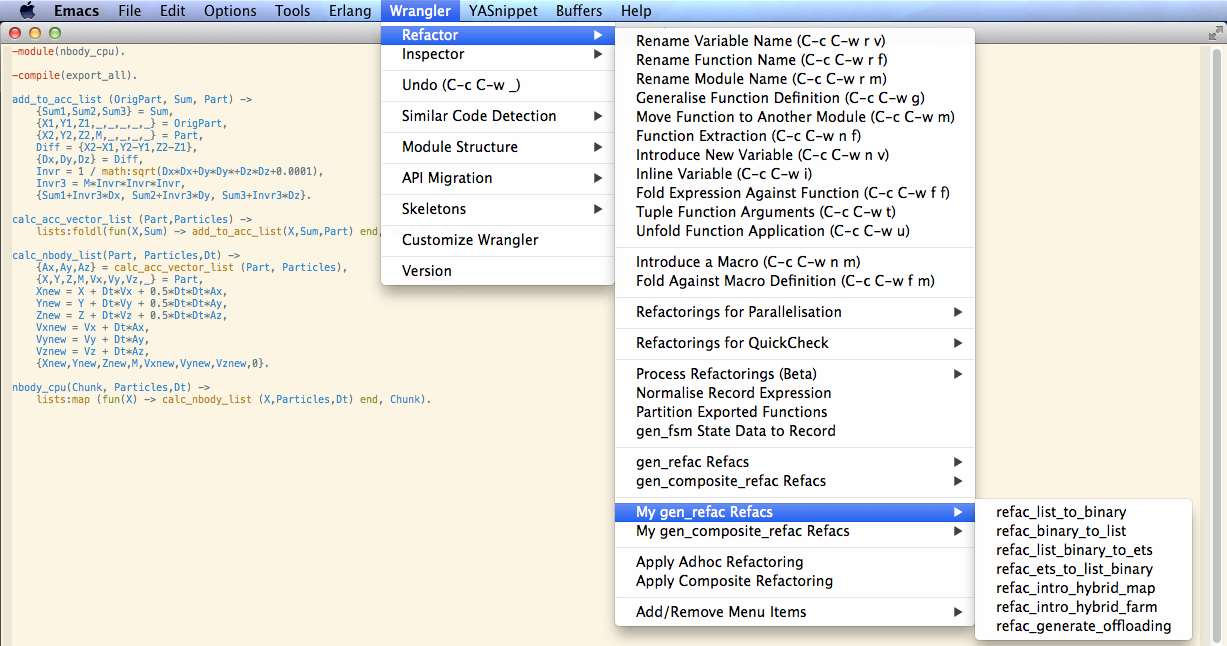
\includegraphics[width=0.9\linewidth]{figures/wrangler_nbody.png}
\caption{Program Shaping and Hybrid Skeleton Refactorings in Wrangler.}
\label{wranglerscreenshot}
\end{center}
\end{figure}

%%%% VJ : This looks like related work to me...Or background
%% \subsection{Refactoring for Parallelism Introduction and Tuning}

%Some recent work has attempted to exploit refactoring technology to
%introduce and tune parallelism.  For example, we have developed
%prototype refactorings for parallel Haskell using the HaRe~\cite{hare} system,
%and also extended Wrangler with a number of novel refactorings to
%%introduce and tune parallelism using skeletons via
%the Skel library~\cite{hlpp}.  We have extended this work to
%introduce and tune skeletons in C/C++~\cite{pdp2014}
%using the FastFlow skeleton library, embedding our refactorings in the
%Eclipse IDE.
%
%In addition to the general advantages above, there are a number of specific %advantages to using refactoring for parallelism
%introduction and tuning:
%%% There are many advantages to parallel refactoring~\cite{ijpp}, some of which we state here (in addition to the advantages of general refactoring as given above):
%\begin{itemize}
%\item Using a refactoring tool to introduce skeletons (instead of
%  manual insertion) means that the programmer has to understand and
%  remember less. This enables them to concentrate more on the
%  design of the program.
%\item A refactoring tool can help minimise changes
% between different releases or implementations of skeletons.
%\item \emph{By design}, a refactoring tool will not allow a user to break %their
%  programs. Introducing an incorrect skeleton, for example, is simply not
%  allowed.
%\end{itemize}

%\noindent
%These advantages are exploited by \Lapedo{} (Section~\ref{lapedoframe}).
%In this paper, we will also take the concept of parallel refactoring further, however: by
%introducing novel refactorings that introduce \emph{hybrid skeletons} (section~\ref{hybrid} for
%heterogeneous systems, and by using refactoring for \emph{program
%  shaping} (Section~\ref{programshaping}).

\iffalse
\subsection{Refactoring for Program Shaping}

% \emph{(Shouldn't this be elsewhere? AB)}

% \begin{itemize}
% \item Skeletons abstract away low-level components, but still require
%   certain things from the program/programmer (examples: list, binary, ets,
%   chunking, task independence)
% \item Programs come in many a different shapes and sizes, thus it is unlikely
%   that all requirements are going to be met
% \item This leads to the programmer often having to change or tune his program to
%   first enable the introduction of skeletons
% \item This stage is often overlooked, and currently only done manually, despite
%   the potentially complex changes that might be applied (examples) (also often
%   requires intimate knowledge of the language and system)
% \item We propose the (semi-)automation of this process through use of
%   refactorings to assist with common edits
% \end{itemize}

% \begin{itemize}
% \item Algorithmic skeletons aim to simplify the introduction of parallelism, by
%   providing a simple, flexible, high-level interface. 
% \item Both parallelism and this interface have a number of requirements (a
%   certain shape) which most programs will not immediately meet. 
% \item Requirements are often extra-functional; memory usage, copying times,
%   independence, and so can be subtle, requiring experience and expertise.
% \item As most programs will not immediately pass all of these, it is often
%   necessary for the programmer to change his program in some way (reshaping).
% \item This program shaping stage is currently done manually, despite potentially
%   complex changes that might be applied, and the often intimate knowledge of
%   language and system that is needed.
% \item We propose the (semi-)automation of this process through the use of
%   refactorings. Refactorings to \emph{enable} the introduction of parallelism
% \end{itemize}

Algorithmic skeletons simplify the introduction of parallelism
by providing a simple high-level interface, abstracting out low-level mechanisms
such as thread creation, synchronisation, and message passing. Whilst
beneficial, this abstraction serves to address a specific problem. Other aspects
of parallelism, such as which part(s) of a program should be parallelised, or
which configuration gives best performance gains, must be similarly addressed.

One common and non-trivial aspect of parallelisation, which heretofore has seen
little interest, is the restructuring of code to enable the introduction of
parallelism~\cite{DBLP:journals/cai/BarwellBHTB16}. Ranging from the detection and breaking of inter-task dependencies,
through changing data representation to avoid excessive memory use, to the
avoidance of scheduler inefficiencies, restructuring to enable parallelism
requires extensive knowledge of the program code, the language used, and
parallelism itself. The complexity of this restructuring, a form of program
shaping, makes it a significant stage of the parallelisation process. Despite
this, however, program shaping remains a manual task, \emph{if it is even
  considered by a parallel development methodology}. Our goal is to use
refactoring to automate and assist with this process as much as possible.

A simple example of program shaping might be to chunk inputs. As
parallelisation involves the introduction of overheads in copying and sending
data between processes, work done on those processes must be sufficiently     large
to outweigh those overheads. Should individual inputs not outweigh those
overheads, inputs might be sent as groups to each worker. Refactoring can be
used to to group, or \emph{chunk}, these inputs. Given the following map
operation is to be parallelised,
% 
\begin{lstlisting}
lists:map(fun f/1, Xs).
\end{lstlisting}
% 
\noindent
where \lstinline|Xs| is a list of inputs to \lstinline|f|. Given also a chunking
function, \lstinline|chunk|:
% 
\begin{lstlisting}
chunk(List, ChunkSize) ->
      case (length(List) < ChunkSize) of
          true -> [List];            
          false -> Chunk = lists:sublist(List, ChunkSize),
                   NewList = lists:sublist(List, ChunkSize+1),
                   [ Chunk | chunk(NewList, ChunkSize) ]
      end.
\end{lstlisting}
% 
\noindent
the \emph{Chunk List} refactoring can transform the map operation by calling
\lstinline|chunk| over \lstinline|Xs|, and introducing a second map over
\lstinline|f|.
%
\begin{lstlisting}
lists:map(fun(Ys) ->
                  lists:map(fun f/1, Ys)
          end, chunk(Xs)).
\end{lstlisting}

Alternatively, should a task farm have already been introduced,
% 
\begin{lstlisting}
skel:do([{farm, [{seq, fun f/1}], NW}], Xs)
\end{lstlisting}
%
\noindent
the \emph{Chunk List} refactoring can transform the farm into a map skeleton
using chunking auxiliary functions provided by Skel.
%
\begin{lstlisting}
skel:do([{map, [{seq, fun f/1}]}], skel:chunk(Xs, N)).
\end{lstlisting}

\fi


% Example: chunking
% Look at generic chunking: i.e. with a map and a chunking function
% (Drum up a rewrite rule for this)
% Look at this in the context of skeletons: we can do this similarly with Skel,
% and automatically introduce a chunking function with it.
% Effects of this -- better more work done on a single worker/process = reduced
% effect of overheads, leading to potentially better performance gains.

% then we go into the new section. (chunking should not be described here.)


% Algorithmic skeletons aim to simplify the introduction of parallelism by
% providing a simple, flexible, and high-level approach. However, in order
% to introduce skeletons successfully, a program must meet a number of pre-conditions, i.e. it must have the right \emph{shape}.
% These pre-conditions derive from quirks of the language/implementation
% (e.g.\@ inefficiencies in handling foreign-function interfaces),
% from extra-functional properties such as memory use and/or time spent copying
% data, as well as from a mismatch between the original structure of the program
% and the desired skeletal structure.
% Since most programs will not have the correct shape, 
% it will be necessary to \emph{shape} the original program before introducing
% parallelism or tuning it to improve performance.
% This can require complex changes to the program, and expert knowledge of the
% language and implementation. Despite this, however, program shaping is
% still considered to be a manual task, \emph{if it is even considered by a
% parallel development methodology.}  This is 
% both tedious and
% error-prone.  Our goal is to use refactoring to automate/assist 
% with this process as much as possible.

% As an example, consider a \lstinline|map| skeleton. Having initially introduced
% a map skeleton, we may decide that the granularity is too fine so that 
% parallel execution cannot compensate for communication overheads, so that 
% increasing the granularity by splitting lists into larger chunks is
% necessary.

\subsection{Refactorings to Introduce Hybrid Skeletons}
\label{sec:hybridRefactorings}

\iffalse
\begin{figure}[t]
\[
  \begin{array}{lrclcl} %% TODO Make a new environment for these
    \rewrite{\Gamma, \s_g \in \bs, n \in \bnp, x,y \in \bnz, m \in
    \brp}{\f}{cluster'(\f, \s_g, n, m, x, y)} \\
    \rewrite{\Gamma, \s_g \in \bs, n \in \brp, g,h,i \in \blf}{\f}{cluster''(\f,
    \s_g, n, g, h, i)}
  \end{array}
\]

% \begin{small}
% \begin{equation*}
% \begin{array}{l}
% \mathit{HybMapIntroSeq}(\rho, \mathtt{e}, g, n_{CPU}, n_{GPU}, s, com) =\\
% \hspace{0.3cm}\mathcal{E}  \llbracket \mathtt{ e } \rrbracket \ \Rightarrow 
%  \llbracket \mathtt{\{map,[\{seq,\ fun(}x\mathtt{)} \rightarrow \\
% \hspace{1.7cm} \mathtt{het}\_\mathtt{map:het}\_\mathtt{dispatcher(lists:map(fun(}y\mathtt{)} \rightarrow c',y\mathtt{))}, g, x\mathtt{)\ end\}]),}\\
% \hspace{1.7cm}\mathtt{fun(}x\mathtt{)} \rightarrow \mathtt{het}\_\mathtt{map:het}\_\mathtt{split(}s, x, n_{CPU}, n_{GPU}\mathtt{)\ end,}\;com\mathtt{\}} \rrbracket \\
% %
% \hspace{0.4cm}\{ \mathtt{seq} \in \rho, \mathtt{map} \in \rho,  g \in \rho, x\
% fresh, y\ fresh, com \in \rho, s \in \rho, c \in \rho,  \\ 
% \hspace{0.4cm}\mathtt{het}\_\mathtt{map} \in imports(\rho), \mathtt{het}\_\mathtt{dispatcher} \in \rho, \mathtt{het}\_\mathtt{split} \in \rho, \overrightarrow{args} = free(c, \rho) \}\\
% where
% \hspace{1em}c' = \llbracket \mathtt{fun(}\overrightarrow{args}\mathtt{)} \rightarrow c \rrbracket , \mathtt{e} = \llbracket \mathtt{ \{seq,\ }c\mathtt{\} } \rrbracket  \\
% \oplus
% % \hspace{0.1cm}\mathcal{E}  \llbracket \mathtt{ e } \rrbracket \ \Rightarrow \\
% \; \llbracket \mathtt{skel:do([\{map,[\{seq,\ fun(}x\mathtt{)} \rightarrow \\
% \hspace{1.4cm} \mathtt{het}\_\mathtt{map:het}\_\mathtt{dispatcher(lists:map(fun(}y\mathtt{)} \rightarrow c',y\mathtt{))}, g, x\mathtt{)\ end\}],}\\
% \hspace{1.4cm}\mathtt{fun(}x\mathtt{)} \rightarrow \mathtt{het}\_\mathtt{map:het}\_\mathtt{split(}s, x, n_{\textsc{CPU}}, n_{GPU}\mathtt{)\ end,\ }com\mathtt{\}], \mathtt{inputs})} \rrbracket \\
% \hspace{0.3cm}\{ \mathtt{seq} \in \rho, \mathtt{map} \in \rho,  g \in \rho, x\
% fresh, y\ fresh, s \in \rho, com \in \rho, c \in \rho, \\
% \hspace{0.5cm} \mathtt{het}\_\mathtt{map} \in imports(\rho),
% \mathtt{het}\_\mathtt{dispatcher} \in \rho,
% \mathtt{het}\_\mathtt{split} \in \rho, \\ 
% \hspace{0.5cm} \mathtt{skel} \in imports(\rho),  \mathtt{do} \in \rho, \mathtt{inputs} \in \rho, \overrightarrow{args} = free(c, \rho) \}\\ 
% where \\
% c' = \llbracket \mathtt{fun(}\overrightarrow{args}\mathtt{)} \rightarrow c
% \rrbracket  \;
% \mathtt{e} = \llbracket \mathtt{ [\ }c(\mathtt{X})\ \mathtt{|\ X} \leftarrow \mathtt{Inputs\ ] } \rrbracket  \vee \llbracket \mathtt{ lists:map(}c,\ \mathtt{Inputs) } \rrbracket \\
%%%
%%\hspace{0.7cm}\{ \mathtt{seq} \in \rho, \mathtt{map} \in \rho,  g \in \rho, x\ fresh, y\ fresh, \mathtt{c} \in \rho, \mathtt{split} \in \rho, \mathtt{com} \in \rho, \mathtt{het}\_\mathtt{map} \in imports(\rho) \\
%%\hspace{0.9cm}\mathtt{het}\_\mathtt{dispatcher} \in \rho, \mathtt{het}\_\mathtt{split} \in \rho, \mathtt{skel} \in imports(\rho), \mathtt{do} \in \rho, \mathtt{inputs} \in \rho \}\\ 
%\oplus
%%
%%\mathit{HybMapIntroComp}(\rho, \mathtt{e}, g, n_{CPU}, n_{GPU}) =\\
%\hspace{0.1cm}\mathcal{E}  \llbracket \mathtt{ e } \rrbracket \ \Rightarrow \\
%\hspace{0.3cm} \llbracket \mathtt{skel:do([\{map,[\{seq, fun(}x\mathtt{)} \rightarrow \mathtt{het}\_\mathtt{map:het}\_\mathtt{dispatcher(lists:map(fun(}y\mathtt{)} \rightarrow \mathtt{c,}y\mathtt{))}, g, x\mathtt{)\ end\}]]),}\\
%\hspace{2.8cm}\mathtt{fun(}x\mathtt{)} \rightarrow \mathtt{het}\_\mathtt{map:het}\_\mathtt{split(s}, x, n_{CPU}, n_{GPU}\mathtt{)\ end,\ com\}]\}], \mathtt{Inputs})} \rrbracket \\
%%
%\hspace{0.7cm}\{ \mathtt{seq} \in \rho, \mathtt{map} \in \rho,  g \in \rho, x\ fresh, y\ fresh, \mathtt{c} \in \rho, \mathtt{split} \in \rho, \mathtt{com} \in \rho, \mathtt{het}\_\mathtt{map} \in imports(\rho) \\
%\hspace{0.9cm}\mathtt{het}\_\mathtt{dispatcher} \in \rho, \mathtt{het}\_\mathtt{split} \in \rho, \mathtt{skel} \in imports(\rho), \mathtt{do} \in \rho, \mathtt{inputs} \in \rho \}\\
%%\oplus
%%%
%%%\mathit{HybMapIntroMap}(\rho, \mathtt{e}, g, n_{CPU}, n_{GPU}) =\\
%%\hspace{0.1cm}\mathcal{E}  \llbracket \mathtt{ lists:map(c, Inputs) } \rrbracket \ \Rightarrow \\
%%\hspace{0.3cm} \llbracket \mathtt{skel:do([\{map,[\{seq, fun(}x\mathtt{)} \rightarrow \mathtt{het}\_\mathtt{map:het}\_\mathtt{dispatcher(lists:map(fun(}y\mathtt{)} \rightarrow \mathtt{c,}y\mathtt{))}, g, x\mathtt{)\ end\}]]),}\\
%%\hspace{2.8cm}\mathtt{fun(}x\mathtt{)} \rightarrow \mathtt{het}\_\mathtt{map:het}\_\mathtt{split(s}, x, n_{CPU}, n_{GPU}\mathtt{)\ end,\ com\}]\}], \mathtt{inputs})} \rrbracket \\
%%%
%%\hspace{0.7cm}\{ \mathtt{seq} \in \rho, \mathtt{map} \in \rho,  g \in \rho, x\ fresh, y\ fresh, \mathtt{c} \in \rho, \mathtt{split} \in \rho, \mathtt{com} \in \rho, \mathtt{het}\_\mathtt{map} \in imports(\rho) \\
%%\hspace{0.9cm}\mathtt{het}\_\mathtt{dispatcher} \in \rho, \mathtt{het}\_\mathtt{split} \in \rho, \mathtt{skel} \in imports(\rho), \mathtt{do} \in \rho, \mathtt{inputs} \in \rho \}\\ 
%where \\
%\mathtt{e} = \llbracket \mathtt{ lists:map(c, Inputs) } \rrbracket  \vee \mathtt{e} = \llbracket \mathtt{ lists:map(c, Inputs) } \rrbracket  \\ 
%\oplus 
%
% \mathit{HybMapIntro}(\rho, \mathtt{e}, g, n_{CPU}, n_{GPU}) =\\
% \hspace{0.3cm}\mathcal{E}  \llbracket \mathtt{ e } \rrbracket \ \Rightarrow \\
% \hspace{0.3cm} \llbracket \mathtt{\{map,[\{seq,\ fun(}x\mathtt{)} \rightarrow \mathtt{het}\_\mathtt{map:het}\_\mathtt{dispatcher(}c', g, x\mathtt{)\ end\}],}\\
% \hspace{1.2cm}\mathtt{fun(}x\mathtt{)} \rightarrow \mathtt{het}\_\mathtt{map:het}\_\mathtt{split(}s, x, n_{CPU}, n_{GPU}\mathtt{)\ end,\ }com\mathtt{\}} \rrbracket\\
% \hspace{0.3cm}\{ \mathtt{seq} \in \rho, \mathtt{map} \in \rho,  g \in \rho, x\ fresh, \mathtt{c} \in \rho, s \in \rho, com \in \rho, \mathtt{het}\_\mathtt{map} \in imports(\rho) \\
% \hspace{0.3cm}\mathtt{het}\_\mathtt{dispatcher} \in \rho, \mathtt{het}\_\mathtt{split} \in \rho, \overrightarrow{args} = free(c, \rho) \}\\
% where 
% \hspace{1em} c' = \llbracket \mathtt{fun(}\overrightarrow{args}\mathtt{)} \rightarrow c \rrbracket ,
% \mathtt{e} = \llbracket \mathtt{ \{map,\ } c\mathtt{,\ }s\mathtt{,\ }com\mathtt{\} } \rrbracket
% \end{array}
% \end{equation*}
% \end{small}
\caption{Refactoring rules for the \emph{Introduce Hybrid Map} refactoring}
\label{hybmapintro}
\end{figure}
\fi

% In this section, we describe refactoring rules that introduce hybrid
% skeletons into sequential or parallel code that contains only
% homogeneous skeletons.

The \emph{Introduce Hybrid Map} (which we also sometimes refer to as \emph{IntroduceHybridCluster}) refactoring is used to insert an instance of a
hybrid cluster.
% 
\[
  \begin{array}{lrclcl} %% TODO Make a new environment for these
    \rewrite{\Gamma, \s_g \in \bs, n \in \bnp, x,y \in \bnz, m \in
    \brp}{\f}{cluster'(\f, \s_g, n, m, x, y)} \\
    \rewrite{\Gamma, \s_g \in \bs, n \in \brp, g,h,i \in \blf}{\f}{cluster''(\f,
    \s_g, n, g, h, i)}
  \end{array}
\]
% 
\noindent
\emph{HybMapIntroSeq} requires
% The refactoring rules for the \emph{Introduce Hybrid Map} refactoring are
% shown in Figure~\ref{hybmapintro}. The refactoring has two rules. The first
% rule, $HybMapIntroSeq$, takes, as arguments to the refactoring,
an environment, $\Gamma$;
% a highlighted expression, \lstinline{e}; 
a skeleton, $\s_g$, that has been generated using the GPU offloading generator
from Section~\ref{sec:gpuCodeGen}; the number of CPU workers, $x$; the
number of GPU workers, $y$; the minimum chunk size $n$; and the CPU to GPU ratio
$m$, which could be generated using, e.g., the work division algorithm described in~\cite{parco2015}. 
% 
%  a function, $s$, that is used to \emph{split}
% the data, and a function, \emph{com}, that is used to \emph{combine} the data.
% The second
% rule, \emph{HybMapIntro}, takes the same arguments as the first rule, omitting the
% user-supplied \emph{split} and \emph{combine} functions.
%
% The first rule, $HybMapIntroSeq$,
The rule matches the highlighted expression,
$\f$, and transforms it into a \lstinline|hyp_cluster| skeleton with appropriate
arguments. 
% , which
% calls the \lstinline{het_map:het_dispatcher} function to schedule the CPU/GPU
% workers, $c$ and $g$. 
% In addition to
% this, the \emph{split} worker in the introduced \lstinline{map} skeleton calls
% the \lstinline{het_map:het_split} function, with $s$, $com$, $n_{CPU}$, and
% $n_{GPU}$ as parameters.
%  the user-supplied
% parameters: $s$, denoting the \emph{split} function; $n_{CPU}$ and $n_{GPU}$,
% denoting the number of CPU and GPU workers, respectively; and, $com$, the
% \emph{combine} function. 
The pre-conditions verify: i) that
the appropriate functions are in scope (i.e., defined within the environment,
$\Gamma$); ii) that the number of CPU and GPU workers may individually be zero,
but must sum to a strictly positive natural number; iii) that the minimum chunk
size is also a strictly positive natural number; and iv) that the CPU to GPU
ratio is a strictly positive real number. 
% that the newly introduced variables, $x$, and $y$ are $fresh$;
% $free(c, \rho)$ means all the free
% variables that are used, but not declared in $c$ or $\rho$. 
% and iii) that the highlighted expression, \lstinline{e}, is either a list
% comprehension, or an application of the \lstinline{lists:map} library function.
%
%
%states that if we have a \lstinline{seq} skeleton wrapping an expression, \lstinline{c}, then we can transform it into a \lstinline{map} skeleton, where the worker function of the map skeleton is the heterogeneous dispatcher (from Section ~\ref{sect:hybrid}), the split function is the user-supplied function, \lstinline{s} (passed as a parameter to the refactoring), and the combine function is the user-supplied function, \lstinline{com} (also passed as a parameter to the refactoring). The remaining refactoring rules in the figure behave in a similar manner. 
% The second rule, $HybMapIntro$, does not require the user-defined \emph{split} and \emph{combine} functions to be provided to the refactoring, and states that if we have an existing \lstinline{map} skeleton (working only for a CPU), then we can also transform it into a hybrid heterogeneous \lstinline{map} skeleton. 
%Likewise, the remaining rules, $HybMapIntroComp$ and $HybMapIntroMap$, state that if we don't yet have an existing skeleton to transform, we may either select a list comprehension of the form stated in $HybMapIntroComp$, or an invocation of the \lstinline{lists:map} function, as stated in the $HybMapIntroMap$ rule, and transform them into a call to \lstinline{skel:do}, instantiated with a hybrid heterogeneous map skeleton. In these two rules, the input list to the list comprehension and to the call to \lstinline{lists:map}, \lstinline{inputs}, becomes the input list to the \lstinline{skel:do}.
%
% show example
%
%
% The second rule is given in \textsc{[url]}, and an example of applying this
% refactoring in Section~\ref{sec:nbody}. 
% As an example of applying this refactoring to introduce a hybrid heterogeneous map, consider that the programmer
% has selected the following for refactoring:
%
% \begin{small}
% \begin{lstlisting}
% [ nbody_cpu:nbody_cpu(Y,Particles,0.0001) | Y <- Particles ] 
% \end{lstlisting}
% \end{small}
%
% \noindent
% The result after refactoring is shown below, where we also further refactor the example
% using the \emph{Introduce New Definition}, refactoring, already supplied in Wrangler~\cite{Li:2008:TSR}. 
% This introduces the variable, \lstinline{Map}, for clarity:
% \begin{small}
% \begin{lstlisting}
% Map = {map, [{seq, fun(X) -> het_map:het_dispatcher(
% 		 fun(Y) ->  nbody_cpu:nbody_cpu(Y,Particles,0.0001) end, 
% 		 fun(Y) ->  nbody_gpu:nbody_gpu(Y,Particles,0.0001) end,
% 		 X) end}],
%            fun(X) -> het_map:het_split(fun split/2,X,NCPU,NGPU) end,
%            fun combine/1},
% skel:do([Map],[Particles]).
% \end{lstlisting}
% \end{small}
%
The second \emph{Introduce Hybrid Map} rewrite rule
acts in a similar way, but serves to instead introduce the second form of the
Hybrid Cluster skeleton.

The \emph{Introduce Hybrid Farm} refactoring is
similar to \emph{Introduce Hybrid Map} and it is used to insert an instance of a hybrid farm.
% 
\[
\begin{array}{rclcl}
  \rewrite{\Gamma, \s_g \in \bs}{\f}{farm'(\f, \s_g)} \\
  \rewrite{\Gamma, \s_g \in \bs, n,m \in \bnz}{\f}{farm''(\f, \s_g, n, m)}
\end{array}
\]
% 
\noindent
It requires an environment, $\Gamma$, a skeleton $\s_g$ that has been generated using the GPU offloading generator from Section~\ref{sec:gpuCodeGen}, and optionally the number of CPU and GPU workers, $n$ and $m$. Unlike in the previous \emph{Introduce Hybrid Map} refactoring, \emph{Introduce Hybrid Farm} does \emph{not} require user-supplied
minimum chunk size or CPU to GPU ratio values.

% \emph{Show this.  KH}

\subsection{Refactorings for Tuning and Type Translation}
\label{sec:shaping}
\label{sect:progshaping}



% In this section, we introduce 
These refactorings do not introduce any
parallelism themselves, but facilitate tuning of parallelism and prepare the original source so that it is easier
to introduce parallelism. Examples may include chunking inputs and
% . Instead, they manipulate data-structures in
% the code, 
altering data representations. These refactorings are useful
%In order to introduce parallelism into a program, typically a program must be \emph{re-shaped}, so 
%that it is structurally altered in order for the parallelism to fit. In this section, we introduce
%some program shaping refactorings that focus on altering the types and the operations on those types within
%Erlang. This is useful 
for improving memory and space usage, and are also required for marshalling data to a GPU.
% , where
% the data must be in a binary form.

%A program might be said to have a \emph{shape}; size, structure, author and
%behaviour all contributing factors. Whilst two programs may be written for
%the same purpose, their shapes may differ greatly, and with this difference,
%performance, memory usage, etc. are affected also. 
%The parallelisation of a
%program requires a certain \emph{shape} before the mechanics of
%parallelism are introduced, and once introduced, the structure used to
%represent data may greatly affect performance. As such, \emph{program reshaping}
%is a common part of the parallelisation process, and currently a manual
%one. Refactoring can be used to automate part of this reshaping, and so speed,
%simplify, and make safe the process. We present two refactorings to help reshape
%data structures.
\subsubsection{Introduce Chunking}
\label{sec:introChunking}

Parallelisation introduces overheads in the form of copying and transmission
costs. To maximise performance gains, these overheads should be kept to a
minimum, and tasks should be large enough to make their copying and transmission worth it.
Should tasks be too small, or are not as large as desired, grouping, or
\emph{chunking}, tasks together can be a simple solution. Chunking can be
accomplished with the aid of the \emph{Introduce Chunking} refactoring~\cite{hlpp}. The
rules for it are shown below.
% 
\[
  \begin{array}{rclcl}
    \rewrite{
    \begin{array}{r}
      \ing{\type{xs}{list}{a}}, \\
      f \in \blf, l \in \bnp
    \end{array}
    }
    {[f(x)\; ||\; x \leftarrow xs]}{skel(map(\f), chunk(xs, l))} \\[2ex]
    \rewrite{\Gamma, l \in \bnp}
    {skel(farm(\s, n), xs)}{skel(map(\s), chunk(xs, l))} \\
  \end{array}
\]
% 
% 
% \begin{small}
% \begin{equation*}
% \begin{array}{l}
% \mathit{IntroChunkComp}(\rho, c, \mathtt{e}) =\\
% \hspace{0.3cm}\mathcal{E}  \llbracket \mathtt{ [ \ f(\  Input\ )  \  ||\  Input} \leftarrow \mathtt{Inputs \ ] } \rrbracket \ \Rightarrow \\
% \hspace{0.3cm} \llbracket \mathtt{ skel:do([ \{ parmap, [\{seq, fun\ ?MODULE:f/1 \}], fun\ skel:partition/1,}\\
% \hspace{5.3cm} \mathtt{ fun\ skel:combine/1\}], skel:chunk(Inputs,}c\mathtt{))} \rrbracket \\
% \hspace{0.7cm}\{ \mathtt{skel} \in \mathtt{imports}(\rho), \mathtt{parmap} \in \rho, \mathtt{run} \in \rho, \mathtt{seq} \in \rho \}\\ 
% \oplus
% \mathit{IntroChunkFarm}(\rho, c, \mathtt{e}) =\\
% \hspace{0.3cm}\mathcal{E}  \llbracket \mathtt{ skel:do([ \{ farm, [\{seq, fun\ ?MODULE:f/1\}], Nw\}], Inputs)   } \rrbracket\ \Rightarrow \\
% \hspace{0.3cm} \llbracket \mathtt{skel:do([ \{ parmap, [\{seq, fun\ ?MODULE:f/1 \}], fun\ skel:partition/1,}\\
% \hspace{5.3cm} \mathtt{ fun\ skel:combine/1\}], skel:chunk(Inputs,}c\mathtt{))} \rrbracket \\
% \hspace{0.7cm}\{ \mathtt{skel} \in \mathtt{imports}(\rho), \mathtt{run} \in \rho, \mathtt{parmap} \in \rho,  \mathtt{seq} \in \rho, \mathtt{farm} \in \rho, \mathtt{Nw} \in \rho\}\\ 
% \end{array}
% \end{equation*}
% \end{small}
% 
The first rule matches a list comprehension, and taking a chunk size $l$,
transforms the comprehension into a call to skel with a \map skeleton over a
\func of the original comprehension function, $f$. The function, \emph{chunk},
is introduced over the original input, $xs$, and takes $l$ as a parameter. The
\emph{chunk} function is provided as part of the skel library; we include its
semantic equivalence rule below.
% 
\[
  \begin{array}{rclcl}
    \seq{\ing{\type{xs}{list}{a}}, l \in \bnp}{chunk(xs,
    l)}{\mathtt{skel:chunk}(xs, l)}
  \end{array}
\]
% 
The second rule may serve to tune already introduced skeletons, matching a task
farm and transforming it into a \map over the skeleton, $\s$ originally nested
within the farm, with the original input chunked in the same manner as the first
rule. 

% \emph{(A tentative suggestion? Have the first chunking rule introduce the
%   chunking but remain in the sequential setting? Perhaps better links it to the
%   `program shaping' idea? AB)}


% The first rule, $IntroChunkComp$, takes, along with an environment, $\rho$, and
% a selected expression, $e$, a chunk size, $c$. The refactoring then matches a
% list comprehension and transforms it into a new \lstinline{parmap} skeleton.
% Here we \emph{chunk} up the tasks in the input list, by calling a function,
% $\mathtt{chunk}$, located in the skeleton library. $\mathtt{chunk}$ is
% parameterised by the input list and the chunk size, and returns a new list of
% tasks, grouped together in sizes of $c$. The function $\mathtt{partition}$
% simply passes the chunks to the map workers and $\mathtt{combine}$ appends the
% results into a result list.
% %
% The second rule, $IntroChunkFarm$, allows the programmer to introduce a chunk
% for a skeleton that is already farmed. In this case, the refactoring simply
% rewrites the \lstinline{farm} skeleton into a \lstinline{parmap}, again with the
% input list chunked into $c$ chunks. It is important to note that, in both of
% these refactoring rules, the function \lstinline{f} remains the same when passed
% as an argument to the \lstinline{parmap} skeleton. Here, the
% \lstinline{partition}, \lstinline{combine} and \lstinline{chunk} functions that
% are introduced are supplied by the Skel library and are defined:

% \begin{small}
% \begin{lstlisting}[numbers=none]
% partition(X) -> X.
% combine([])->[];
% combine([X|Xs]) -> lists:append(X, recomp(Xs)).
% chunk([], ChunkSize) -> [];
% chunk(List, ChunkSize) ->
%       case (length(List) < ChunkSize) of
%           true -> [List];            
%           false -> Chunk = lists:sublist(List, ChunkSize),
%                    NewList = lists:sublist(List, ChunkSize+1),
%                    [ Chunk | chunk(NewList, ChunkSize) ]
%       end.
% \end{lstlisting}
% \end{small}

% Here, \lstinline{chunk} groups together \lstinline{ChunkSize} elements in a
% list; \lstinline{partition} acts as the identity function (in the
% \lstinline{parmap} skeleton, the \lstinline{partition} function decomposes a
% single element of the input stream; in this case a single element is a group of
% elements (a chunk) where we want each worker thread to operate over a whole
% chunk, and so we disable the partition function by using the identity instead),
% and \lstinline{combine} concatenates the partitioned results into a single list.


\vspace{-6pt}
\subsubsection{List to Binary.}
\vspace{-6pt}
\label{sec:listToBinary}
The Erlang concurrency model is
\emph{shared-nothing}. %, there is no shared data between processes
This means that all data must be copied between processes. One exception being
\emph{binaries}, which are normally passed by reference.
% . These are not copied between process, but rather
% only references to them are copied.
% If a list is shared, 
Converting a list that is shared between processes to a binary form can have a significant
positive impact on performance, since only the reference to the binary is copied between processes and not the data~\cite{Barwell:2016:TSD}.
% parallel application, as this can save a lot of copying of the data if
% the list is shared. Converting list to binary
Conversion is also necessary when marshalling data to a GPU kernel.
% Conversion is also necessary if a list needs to be passed to a GPU kernel.
% need to operate on lists, as kernels only ``understand'' binaries. The rewrite
% rules for performing the \emph{Transform List to Binary} refactoring are shown
% in Figures~\ref{fig:listtobinary}--\ref{fig:listtobinaryexpr2}.
% \ref{eq:ltob1}, \ref{eq:ltob2}, and \ref{eq:ltob3}.

Conversion between two data representations, such as lists and binaries, is made
non-trivial in Erlang through a combination of differences in APIs between the
two representations, and Erlang's dynamic typing. The latter allowing each
element in lists and other collection types to be of a different type.
Accordingly, the programmer must know the type of each of the elements in the
list to be transformed, in addition to the differences in API. Further still,
should one part be changed to a different representation, the programmer must
manually follow and transform all statements affected by that one
transformation, a process during which error can easily be introduced and go
unnoticed during compilation.

A list to binary refactoring has been developed to address these problems~\cite{Barwell:2016:TSD}.
The top-level rewrite rule for the refactoring is given below.
% 
\[
  \begin{array}{rclcl}
    \Rewrite{\ing{x}}{\mathcal{E}_{\type{x}{list}{a}}}{\mathcal{E}_{\type{x}{binary}{a}} }
  \end{array}
\]
% 
The refactoring takes as argument a variable, $x$, of type list whose elements
are of all the same type, to be transformed to a binary whose elements are of
the same type and size. The rule discovers the set of all statements that define
or influence $x$, denoted $\mathcal{E}$, and transforms them through application
of a series of rewrite rules to their binary equivalents. This refactoring is a
composite refactoring, meaning it applies a series of sub-rewrite rules in turn
to each statement in such a way that the overarching change does not break
functional correctness.
% 
% \emph{(Should a couple of these be shown? AB)}


% Top-level rewrite rules for the \emph{Transform List to Binary} refactoring are
% shown in Figure~\ref{fig:listtobinary}. Full rules can be found in
% Appendix~\ref{sec:refacrules}. \emph{We should say this earlier, then delete
%   this comment. KH}
%
% The rewrite
% rules for performing the \emph{Transform List to Binary} refactoring can be
% found in equations \ref{eq:ltob1}, \ref{eq:ltob2}, and \ref{eq:ltob3}.
%
% Converting lists to binary data structures is desirable to reduce copying
% The refactoring rules for transforming a function over lists into
% a function over a binary can be found in % the following
% equations \ref{eq:ltob1},~\ref{eq:ltob2}, and~\ref{eq:ltob3}. 
%The rule
%featured in Equation~\ref{eq:ltob1}, \textit{ListToBinary}, presents a point of
%entry for the refactoring described.
%
% \begin{figure}[t]
% \begin{small}
% \begin{equation*} \label{eq:ltob1}
% \begin{array}{l}
% ListToBinary(\rho, \mathtt{f}, \mathtt{Arg}, \mathtt{T}, \overrightarrow{types}) = \\
% \hspace{1em} \mathcal{D} \qquote{\mathtt{f}} \Rightarrow \qquote{\mathtt{f(}
%   \overrightarrow{x}, \mathtt{Arg}', \overrightarrow{z}) \rightarrow \overrightarrow{body}'} \\
% \cond{\inenv{\mathtt{f}}, \inenv{\overrightarrow{x}},
%   \inenv{\overrightarrow{z}}, \inenv{\mathtt{Arg}}, \mathtt{T} \not\in \rho}  \\
% \hspace{0.5em} where \\
% \hspace{2em} \mathtt{Arg}' = ListToBinaryExpr(\rho, \mathtt{Arg}, \mathtt{T},
% \overrightarrow{types}) \\ 
% \hspace{2em} \overrightarrow{body}' = ListToBinaryExpr(\rho,
% \overrightarrow{body}, \mathtt{T}, \overrightarrow{types}) \\ 
% \hspace{2em} \mathtt{f} = \qquote{\mathtt{f}(\overrightarrow{x}, \mathtt{Arg},
%   \overrightarrow{z}) \rightarrow \overrightarrow{body}}
% \end{array}
% \end{equation*}
% \end{small}
% \caption{Top-level refactoring rule for the \emph{Transform List to Binary} refactoring}
% \label{fig:listtobinary}
% \end{figure}
%
% \textit{ListToBinary} takes as its arguments: an environment, $\rho$; the
% function to be operated over, \lstinline{f}; the list, \lstinline{Arg}; an
% unbound variable name \lstinline{T}; and $\overrightarrow{types}$,
% used as part of Erlang's bit syntax for determining
% which indicates the type of individual binary elements.
% To perform the refactoring, given a set of
% arguments, \emph{ListToBinary} 
% It first transforms \lstinline{Arg}, then the body of \lstinline{f}.
% , using \emph{ListToBinaryExpr} (see  \textsc{[url]}).
% \emph{ListToBinary} takes as argument: an environment, $\rho$; a function,
% \lstinline{f}, in $\rho$ to be operated over; an argument, \lstinline{Arg}, to \lstinline{f}
% of type list; an unbound variable name \lstinline{T}; and $\overrightarrow{types}$, for
% indicating the type of individual list/binary elements. Given a set of
% arguments, \emph{ListToBinary} transforms both \lstinline{Arg} and the body
% of \lstinline{f} using the rule \emph{ListToBinaryExpr}. \emph{ListToBinaryExpr}
% (given in \textsc{[url]}) matches against the shape of \lstinline{Arg},
% applying the appropriate transformation. The process is similarly repeated for
% each statement in the body of \lstinline{f}. 

% % \textit{ListToBinary} takes, as argument, an environment,
% % $\rho$; the function to be operated over, \lstinline{f}; a list argument to
% % \lstinline{f}, denoted \lstinline{Arg}; a variable name \lstinline{T}; and
% % $\overrightarrow{types}$, used as part of Erlang's bit syntax for determining
% % the type of binary elements. To perform the refactoring, given a set of
% % arguments, \emph{ListToBinary} first transforms \lstinline{Arg}, then the body of
% % \lstinline{f}. These transformations are performed by calling
% % \emph{ListToBinaryExpr} on both.
% >>>>>>> .r3807
%\vspace{-60pt}
%
% \begin{figure}[t]
% \begin{small}
% \begin{equation} \label{eq:ltob2}
% \begin{array}{l}
% ListToBinaryExpr(\rho, \mathtt{Arg}, \mathtt{T}, \overrightarrow{types}) = \\
% \hspace{1em} \mathcal{E} \qq{Arg} \Rightarrow \qq{T =
%   g\mathit{'}(\mathit{\overrightarrow{y}}), <<\mathit{\overrightarrow{x}}, T/binary>>} \\
% \cond{\inenv{\mathtt{Arg}}, \inenv{\mathtt{g}}, \inenv{\overrightarrow{x}},
%   \inenv{\overrightarrow{y}}, \mathtt{T} \not\in \rho} \\
% \hspace{0.5em} where \\
% \hspace{1em} \mathtt{g}' = ListToBinaryExpr(\rho, \mathtt{Arg}, \mathtt{T},
% \overrightarrow{types})\ ,\  \mathtt{Arg} = \qq{[\,\mathit{\overrightarrow{x}}\, |\,
%   g(\mathit{\overrightarrow{y}}) ]} \\ 
% %
% \hspace{.2em} \oplus \, \mathcal{E} \qq{e} \Rightarrow
% \qq{n:h(\mathit{\overrightarrow{x}}, Arg, \mathit{\overrightarrow{z}})} \\
% \cond{\inenv{\overrightarrow{x}}, \inenv{\overrightarrow{z}},
%   \inenv{\mathtt{g}}} \\
% \hspace{0.5em} where \\
% \hspace{2em} \mathtt{n:g} = ListToBinaryExpr(\rho, \mathtt{Arg}, \mathtt{T},
%   \overrightarrow{types}) , \ 
% \mathtt{e} = \qq{m:g(\mathit{\overrightarrow{x}}, Arg, \mathit{\overrightarrow{z}})} \\
% %
% \hspace{.2em}\oplus \, \mathcal{E} \qq{e} \Rightarrow
% \qq{g\mathit{'}(\mathit{\overrightarrow{x}}, Arg\mathit{'}, \mathit{\overrightarrow{z}})} \\
% \cond{\inenv{\mathtt{g}}, \inenv{\overrightarrow{x}}, \inenv{\overrightarrow{z}}} \\ 
% \hspace{0.5em} where \\
% \hspace{2em} \mathtt{g}' = ListToBinaryExpr(\rho, \mathtt{Arg}, \mathtt{T},
% \overrightarrow{types}) \\
% \hspace{2em} \mathtt{Arg}' = ListToBinaryExpr(\rho, \mathtt{Arg}, \mathtt{T},
% \overrightarrow{types}) \\
% \hspace{2em} \mathtt{e} = \qq{g(\mathit{\overrightarrow{x}}, Arg, \mathit{\overrightarrow{z}})} \\
% %
% \hspace{.2em} \oplus \, \mathcal{E} \qq{e} \Rightarrow
% \qq{lists:\mathit{y}(fun(\mathit{arg}) \rightarrow
%   \mathit{\overrightarrow{body}'}\, end, \mathit{\overrightarrow{params}'})} \\
% \cond{\inenv{\mathtt{Arg}}, \inenv{\mathtt{Acc}}, \inenv{\overrightarrow{body}}, \inenv{arg},
% \inenv{z}} \\
% \hspace{.5em} where \\
% \hspace{2em} y = \qq{map} \lor \qq{foldl} \\
% \hspace{2em} \overrightarrow{params}' = b \lor ListToBinaryExpr(\rho,
% a, \mathtt{T}, \overrightarrow{types}), b \\
% \hspace{2em} \overrightarrow{body}'  = ListToBinaryExpr(\rho, \mathtt{Arg},
% \mathtt{T}, \overrightarrow{types}) \\
% \hspace{2em} \mathtt{e} = \qq{lists:map(fun(Arg) \rightarrow
%   \mathit{\overrightarrow{body}} \, end, \mathit{b})} \, \lor  \\
% \hspace{4em} \qq{lists:foldl(fun(Arg, Acc) \rightarrow \mathit{\overrightarrow{body}} \, end,
%   \mathit{a}, \mathit{b})} \\
% %
% \hspace{.2em} \oplus \, \mathcal{E} \qq{e} \Rightarrow \qq{Arg\mathit{'}} 
% \cond{\inenv{\mathtt{e}}} \\
% \hspace{1em} where 
% \hspace{1em} \mathtt{Arg}' = ListToBinaryExpr(\rho, \mathtt{Arg},
%   \overrightarrow{types})
% \end{array}
% \end{equation}
% \end{small}
% \caption{Inner rewrite rules for the \emph{Transform List to Binary} Refactoring.}
% \label{fig:listtobinaryexpr1}
% \end{figure}
%\vspace{-3cm}

% \noindent
% The \emph{ListToBinaryExpr} rule % is first given in Equation~\ref{eq:ltob2}
% % and
% takes the same arguments as \emph{ListToBinary} except that \lstinline{Arg}
% represents either the original argument or the body of \lstinline{f}. 
% When given the original argument, \emph{ListToBinaryExpr} matches its shape,
% and applies the appropriate rewrite. 
% \emph{ListToBinaryExpr} is applied recursively to each statement in the body of \lstinline{f}.
% This refactoring requires that \lstinline{f} must be available in $\rho$, and that
% \lstinline{Arg} represents not only a list, but is an argument to \lstinline{f}. Where
% \lstinline{T} is required, \lstinline{T} must not already be in $\rho$.

% Just as
% \emph{ListToBinary} invokes \emph{ListToBinaryExpr}, \emph{ListToBinaryExpr}
% may invoke itself again, or the \emph{ListToBinaryExpr} given in
% Equation~\ref{eq:ltob3}, requiring \lstinline{T} as argument.

% The rule, \emph{ListToBinaryExpr}, is first given in Equation~\ref{eq:ltob2}
% and takes the same arguments as \emph{ListToBinary} except for \lstinline{Arg}, now
% representing either the original argument or the body of \lstinline{f}. In case of
% the original argument, \emph{ListToBinaryExpr} matches against its shape,
% applying the appropriate rewrite. When applied to the body of \lstinline{f},
% \emph{ListToBinaryExpr} applies itself to each statement in that body. Just as
% \emph{ListToBinary} invokes \emph{ListToBinaryExpr}, \emph{ListToBinaryExpr}
% may invoke itself again, or the \emph{ListToBinaryExpr} given in
% Equation~\ref{eq:ltob3}, requiring \lstinline{T} as argument.
%
% \begin{figure}[t]
% \begin{small}
% \begin{equation} \label{eq:ltob3}
% \begin{array}{l}
% ListToBinaryExpr(\rho, \mathtt{Arg}, \overrightarrow{types}) = \\
% \hspace{1em} \mathcal{E} \qq{e} \Rightarrow
% \qq{lists:\mathit{y}(\mathit{a}, binary\_to\_list(Arg))} \\
% \cond{\inenv{\mathtt{Arg}}, \inenv{a}, \inenv{y}} \\
% \hspace{0.5em} where 
% \hspace{1em} y = \qq{map} \lor y = \qq{foldl} , \ 
% \mathtt{e} = \qq{lists:\mathit{y}(\mathit{a}, Arg)} \\
% %
% \hspace{.2em} \oplus \, \mathcal{E} \qq{Arg} \Rightarrow
% \qq{<<\mathit{\overrightarrow{x}}/\mathtt{\overrightarrow{types}}, T/binary>>} \\
% \cond{\inenv{\mathtt{Arg, T}}, \inenv{\overrightarrow{x}}} 
% \hspace{.5em} where 
% \hspace{.5em} \mathtt{Arg} = \qq{[\,\mathit{\overrightarrow{x}}\,|\, T\,]} \\
% %
% \hspace{.2em} \oplus \, \mathcal{E} \qq{Arg} \Rightarrow \qq{\mathit{x}} \\
% \cond{\inenv{\mathtt{Arg}}, \inenv{x}} 
% \hspace{.5em} where 
% \hspace{.5em} \mathtt{Arg} = \qq{binary\_to\_list(\mathit{x})} \\
% %
% \hspace{.2em} \oplus \, \mathcal{E} \qq{Arg} \Rightarrow
% \qq{<<\mathit{\overrightarrow{x}}/\mathit{\overrightarrow{types}}>>} \\
% \cond{\inenv{\mathtt{Arg}}, \inenv{\overrightarrow{x}}} 
% \hspace{.5em} where 
% \hspace{.5em} \mathtt{Arg} = \qq{[\,\mathit{\overrightarrow{x}}\,]} \\
% % 
% \hspace{.2em} \oplus \, \mathcal{E} \qq{Arg} \Rightarrow \qq{<<>>} 
% \cond{\inenv{\mathtt{Arg}}} 
% \hspace{.5em} where 
% \hspace{.5em} \mathtt{Arg} = \qq{[\,]} \\
% %
% %\hspace{.2em} \oplus\,  \mathcal{E} \qq{Arg} \Rightarrow \qq{Arg} 
% %\hspace{-.5em} \cond{\inenv{\mathtt{Arg}}} 
% \end{array}
% \end{equation}
% \end{small}
% \caption{Inner rewrite rules for the \emph{Transform List to Binary} refactoring}
% \label{fig:listtobinaryexpr2}
% \end{figure}
%
% This refactoring requires that \lstinline{f} must be available in $\rho$, and that
% \lstinline{Arg} represents not only a list, but is an argument to \lstinline{f}. Where
% \lstinline{T} is required, \lstinline{T} must not already be in $\rho$.

%\pagebreak
In order to illustrate this refactoring, consider the \lstinline{get_particles} function:
% 
\begin{lstlisting}
get_particles(Data) ->
     lists:foldl(fun(X, Acc) -> {Str, _} = string:to_float(X),
                                [Str | Acc] end,
                 [],string:tokens(Data," ")).
\end{lstlisting}
% 
\noindent
This is part of our N-Body example from Section~\ref{sec:nbody}. It takes a
string, \lstinline{Data}, that contains space-separated floating-point numbers,
and returns a list of these numbers. Suppose that, instead of a list, we require
\lstinline{get_particles} to return a binary.
% of floating-point numbers. \emph{ListToBinary} can be applied to
% \lstinline{get_particles} function, as it returns a list.
We can achieve this by applying \emph{ListToBinary} to the body of
\lstinline{get_particles}:
% %
% This function takes the string argument, \lstinline{Data}, containing
% space-separated floating point numbers. 
% % This function takes as argument a string \lstinline{Data} containing
% % space-separated floating point numbers. 
% Suppose that, instead of a list, we want
% \lstinline{get_particles} to return a binary of floating point
% numbers. \emph{ListToBinary} can be applied to \lstinline{get_particles}, as it
% returns a list. This application results in the following code:
% %
% % Applying this refactoring results in the following code:
% %
% 
\begin{lstlisting}
get_particles(Data) ->
     lists:foldl(fun(X, Acc) -> {Str, _} = string:to_float(X),
                                T = <<Str/float>>,
                                <<T/binary, Acc/binary>> end,
                                <<>>, string:tokens(Data, " ")).
\end{lstlisting}
% 
% To illustrate the above refactoring, consider the following function
% (a part of our N-Body use case, presented in more details in
% Section~\ref{sec:nbody}):
% \begin{lstlisting}
% get_particles(Data) ->
%      lists:foldl(fun(X, Acc) -> {Str, _} = string:to_float(X),
%                                 [Str | Acc] end,
%                  [],string:tokens(Data," ")).
% \end{lstlisting}
% This function takes as an argument a string \lstinline{Data} that
% contains space-separated float numbers, and returns a list of these
% numbers. Suppose that, instead of a list, we want
% \lstinline{get_particles} to return a binary of float numbers. 
% \emph{ListToBinary} can be applied to \lstinline{get_particles}
% function, as it returns a list. Applying this refactoring results in
% the following code:
% \begin{lstlisting}
% get_particles(Data) ->
%      lists:foldl(fun(X, Acc) -> {Str, _} = string:to_float(X),
%                                 T = <<Str/float>>,
%                                 <<T/binary, Acc/binary>> end,
%                                 <<>>, string:tokens(Data, " ")).
% \end{lstlisting}


% programmer desires to change \lstinline{start} such that the list
% \lstinline{Particles} is instead stored as a binary. The programmer might therefore
% apply \emph{ListToBinary} to both \lstinline{init} and \lstinline{do_nbody}. %We give these functions below.

% To illustrate the above refactoring, we use our running example. Suppose the
% programmer desires to change \lstinline{start} such that the list
% \lstinline{Particles} is instead stored as a binary. The programmer might therefore
% apply \emph{ListToBinary} to both \lstinline{init} and \lstinline{do_nbody}. %We give these functions below.

% \begin{small}
% \begin{lstlisting}
% start() ->      
%     Particles = init("input_data"),
%     do_nbody(Particles).
% init(Fname) ->
%    ...
% 	{ok, Data} -> get_particles(Data);
%    ...
% do_nbody(Particles) ->
%     [nbody_cpu:nbody_cpu(Y, Particles, 0.0001) | Y <- Particles].
% \end{lstlisting}
% \end{small}

% \noindent
% The programmer might first apply
% \emph{ListToBinary} to \lstinline{init}, as it is the function producing \lstinline{Particles}.
% % Within \lstinline{init/1}, two functions
% %are of interest to the refactoring; no change is affected to
% %\lstinline{file:read\textunderscore line}, the case block, or
% %variables, meaning no change is affected to \lstinline{init/1} itself.
% %
% \emph{ListToBinary} affects no changes within \lstinline{open_file}, but transforms \lstinline{get_particles}, shown below.
% \begin{small}
% \begin{lstlisting}
% get_particles(Data) ->
%     lists:foldl(fun(X, Acc) -> {Str, _} = string:to_float(X),
% 			          [Str | Acc] end,[],string:tokens(Data," ")).
% \end{lstlisting}
% \end{small}
% \noindent
% Here, \emph{ListToBinary} enters the \lstinline{foldl}, changing the initial value, and
% return value of the anonymous function. 

% \begin{small}
% \begin{lstlisting}
% get_particles(Data) ->
%     lists:foldl(fun(X, Acc) -> {Str, _} = string:to_float(X),
% 			          T = <<Str/float>>,
% 			          <<T/binary, Acc/binary>> end,
% 		                  <<>>, string:tokens(Data, " ")).
% \end{lstlisting}
% \end{small}
% %
% %This completes the refactoring over \lstinline{init/1}. Applying now the
% %refactoring to \lstinline{do\textunderscore nbody}, \emph{ListToBinary} repeats the
% %process. Again, \lstinline{do\textunderscore nbody} itself remains unchanged. The
% %function \lstinline{calc\textunderscore to\textunderscore acc\textunderscore
% %  list/3}, invoked as part of \lstinline{do\textunderscore nbody} is transformed,
% %adding a call to \lstinline{binary\textunderscore to\textunderscore list/1},
% %resulting in the following.
% %
% %\begin{small}
% %\begin{lstlisting}
% %calc_acc_vector_list (Part, Particles) ->
% %    lists:foldl(fun(X,Sum) -> add_to_acc_list(X,Sum,Part) end, 
% %		                {0,0,0}, binary_to_list(Particles)).
% %\end{lstlisting}
% %\end{small}


% \vspace{-6pt}
% \subsubsection{List/Binary to ETS Table.}
% \vspace{-6pt}
% \label{sec:listToETS}
% Erlang's \emph{ETS} tables provide a single shared, updatable structure, that is
% designed to store large amounts of data.
% % As binaries, ETS tables are not copied between Erlang processes. 
% ETS tables can be updated much more easily and quickly than binaries, without
% the need to create a new data structure. However, they are not thread safe:
% multiple processes can simultaneously modify the same part of the table. ETS
% tables should therefore only be used when it is possible to ensure the
% consistency of reads and updates. We can define a \emph{Transform List
%   to ETS Table} that is similar to \emph{ListToBinary}.


% \emph{Give this or omit the subsection. KH}
% The details are omitted here (they are given in Appendix~\ref{sec:refacrules}).
% Using ETS tables instead of 
%
% The \emph{Transform List or Binary to ETS Table} refactoring is simu. We omit the
% details here, and instead refer interested reader to...We will show 
%but we show an example of this refactoring in Section~\ref{sec:nbody}.

%%% VJ: I will comment this out for now, as we definitely do not have
%%% 3 pages to dedicate to refactoring that we don't even use in the
%%% examples

% The conversion to use Erlang's \textsc{ets} tables provides a single, updatable
% structure designed for the storage of large amounts of data, helping to reduce
% the amount of data copied.
% The rules for the \emph{Transform List or Binary to ETS Table} refactoring may be found in
% Equation~\ref{eq:lbtoets}. As with the refactoring in the previous section,
% \emph{ListBinaryToETS} is invoked by the programmer, and the rule invoking
% others. \emph{ListBinaryToETS} takes, as argument, an environment, $\rho$; a
% module, $M$, in which the refactoring is focussed; two
% functions \lstinline{f} and \lstinline{d} within $\rho$ to guide the refactoring; a
% function \lstinline{r}, providing the means to recover and reformat inputs placed
% in the \textsc{ets} table; a function \lstinline{i} to wrap inputs in a tuple and
% add a unique identifier as the first element; a name for the table,
% \lstinline{TName}; a name for the aforementioned identifier element,
% \lstinline{IName}; and lastly, a list or binary term, denoted \lstinline{Term}. 
% The \emph{ListBinaryToETS} rule represents a composite refactoring, and, as such,
% invokes four other rules: \emph{IntroCreateFun}, \emph{WrapWithCAndR},
% \emph{IntroIDWrapperFun}, and \emph{TabIntro}. 
%These rules are invoked in order, by using the $\comp$ operator, 
%and should any one of these rules fail, \emph{ListBinaryToETS} fails also,
%affecting no change to the program to which it is applied.
%
% The rule \emph{IntroCreateFun}, once invoked, introduces a function to $M$ to
% instantiate the \textsc{ets} table to be used. The table is given
% the name \lstinline{TName}, along with the following configuration.

% \begin{figure}[!t]
% \begin{small}
% \begin{equation} \label{eq:lbtoets}
% \begin{array}{l}
% ListBinaryToETS(\rho, M, \mathtt{f}, \mathtt{r}, \mathtt{d}, \mathtt{i}, \mathtt{TName},
% \mathtt{IName}, \mathtt{Term}) = \\
% \hspace{1em} IntroCreateFun(\rho, M, \mathtt{TName}) \comp WrapWithCAndR(\rho,
% \mathtt{f}, \mathtt{r}) \comp \\
% \hspace{2em} IntroIDWrapperFun(\rho, \mathtt{i}, \mathtt{Term}) \comp
% TabIntro(\rho, \mathtt{d}, \mathtt{TName}, \mathtt{IName}) \\
% \cond{\inenv{M}, \inenv{\mathtt{f}}, \inenv{\mathtt{d}}, \inenv{\mathtt{r}},
%   \inenv{\mathtt{i}}, \inenv{\mathtt{Term}}, \ninenv{\mathtt{IName}},
%   \mathtt{TName} \not\in \mathtt{tables}(\rho)} \\
% %
% TabIntro(\rho, \mathtt{d}, \mathtt{TName}, \mathtt{IName}) = \\
% \hspace{1em} InsertRetToETS(\rho, \mathtt{d}, \mathtt{TName}, \mathtt{IName})
% \comp WrapWorkerFun(\rho, \mathtt{g}, \mathtt{TName}, \mathtt{IName}) \\
% \cond{\inenv{\mathtt{d}}, \mathtt{TName} \in \mathtt{tables}(\rho),
%   \inenv{\mathtt{IName}}} \\ 
% \hspace{0.5em} where 
% \hspace{.5em} \mathtt{g} = \mathtt{d} \leadsto \mathtt{g} \\
% %
% %
% IntroCreateFun(\rho, M, \mathtt{TName}) = \\
% \hspace{1em} \mathcal{M} \qq{\mathit{M}} 
%  \Rightarrow \qquote{\overrightarrow{macro},\,\mathtt{create()
%     \rightarrow TName = ets:new(TName,[set, public, named\_table, } \\
% \hspace{2em} \mathtt{\{write\_concurrency, true\}, \{read\_concurrency,
%   true\}]).,}\, \overrightarrow{dec}} \\
% \cond{\inenv{M}, \inenv{\overrightarrow{macro}}, \inenv{\overrightarrow{dec}},
%   \mathtt{create/0}, \not\in \mathtt{decs}(M), \mathtt{TName} \not\in
%   \mathtt{tables}(\rho)} \\
% \hspace{0.5em} where 
% \hspace{.5em} M = \qq{\mathit{\overrightarrow{macro}}, \mathit{\overrightarrow{dec}}} \\
% %
% WrapWithCAndR(\rho, \mathtt{f}, \mathtt{r}) = \\
% \hspace{1em} \mathcal{D} \qq{\mathit{x}} \Rightarrow
%   \qq{f(\mathit{\overrightarrow{y}}) \Rightarrow
%     create(),\,\mathit{\overrightarrow{body}},\,\mathtt{r}} \\ 
% \cond{\inenv{\mathtt{f}}, \inenv{\mathtt{r}}, \inenv{\overrightarrow{y}},
%   \inenv{\overrightarrow{body}}} 
% \hspace{0.5em} where 
% \hspace{.5em} x = \qq{f(\mathit{\overrightarrow{y}}) \rightarrow
%   \mathit{\overrightarrow{body}}} \\
% %
% IntroIDWrapperFun(\rho, \mathtt{i}, \mathtt{Term}) = \\
% \hspace{1em} \mathcal{E} \qq{\mathit{x}} \Rightarrow \qq{i(Term)} \\
% \cond{\inenv{\mathtt{i}}, \inenv{\mathtt{Term}}} \\
% \hspace{0.5em} where 
% \hspace{.5em} x = \mathtt{Term} \\
% %
% InsertRetToETS(\rho, \mathtt{d}, \mathtt{TName}, \mathtt{IName}) = \\
%  \mathcal{D} \qq{d} 
%  \Rightarrow \qq{d(\{IName, \mathit{\overrightarrow{x}}\})
%   \rightarrow \mathit{\overrightarrow{body}},\, ets:insert\_new(TName,
%   \{IName, \mathit{body_n}\}), IName} \\
% \cond{\inenv{\mathtt{d}}, \mathtt{TName} \in \mathtt{tables}(\rho),
%   \inenv{\mathtt{IName}}, \inenv{\overrightarrow{x}},
%   \inenv{\overrightarrow{body}}, \inenv{body_n}} \\
% \hspace{0.5em} where 
% \hspace{.5em} \mathtt{d} = \qq{d(\mathit{\overrightarrow{x}}) \rightarrow
%   \overrightarrow{body}, \mathit{body_n}} \\
% %
% WrapWorkerFun(\rho, \mathtt{g}, \mathtt{TName}, \mathtt{IName}) = \\
% \hspace{1em} \mathcal{D} \qq{g} 
%  \Rightarrow \qquote{\mathtt{g(IName) \rightarrow [\{IName,
%     \mathit{x}\}] = ets:lookup(TName, IName),\, \mathit{\overrightarrow{body}},}
%   \\\hspace{3em}
%   \mathtt{ets:insert(TName, \{IName, \mathit{body_n}\}), IName}} \\
% \cond{\inenv{\mathtt{g}}, \mathtt{TName} \in \mathtt{tables}(\rho),
%   \inenv{\mathtt{IName}}, \inenv{x}, \inenv{\overrightarrow{body}},
%   \inenv{body_n}} \\
% \hspace{0.5em} where 
% \hspace{.5em} \mathtt{g} = \qq{g(\mathit{x}) \rightarrow \overrightarrow{body},
%   \mathit{body_n}} \\ 
% \end{array}
% \end{equation}
% \end{small}
% \caption{Rewrite rules for the \emph{Transform List or Binary to ETS Table} refactoring}
% \label{fig:listbinarytoets}
% \end{figure}

% \begin{small}
% \begin{lstlisting}
% [set, public, named_table, 
%   {write_concurrency, true}, {read_concurrency, true}]
% \end{lstlisting}
% \end{small}

% \noindent
% This configuration helps to avoid any complications produced through duplicate
% entries with the \lstinline{set} option. It allows all workers to access the table,
% and that table be accessible via name, through \lstinline{public} and
% \lstinline{named_table}. The options \lstinline{write_concurrency} and \lstinline{read_concurrency} are set to true for
% efficiency. \emph{WrapWithCAndR} then introduces a call to the aforementioned
% function at the beginning of the body of \lstinline{f}, and the restoration
% function \lstinline{r} at its end. \emph{IntroIDWrapperFun} is employed to find
% \lstinline{Term}, and wrap a call to \lstinline{i} about it. \emph{TabIntro} is then
% invoked, itself invoking two other rules. \emph{TabIntro} first invokes
% \emph{InsertRetToETS} over the function \lstinline{d}, allowing \lstinline{d} to
% first introduce its original output values to \lstinline{TName}. Each function
% that takes \lstinline{d}'s output, directly or indirectly, is edited by
% \emph{WrapWorkerFun}. \emph{WrapWorkerFun} edits a function to receive
% \lstinline{IName} as input and return value, also adding a table lookup at the
% start of the body of the function, and updating the table contents using the
% original return value.
% %
% To invoke \emph{ListBinaryToETS} a number of conditions must be
% met. \lstinline{Term} must be in the body of \lstinline{f}, which must be defined in
% $M$. The function \lstinline{r} must be provided by the programmer to extract
% the contents of \lstinline{TName}, and remove any changes imposed on the contents'
% formatting. Similarly, \lstinline{i} must be provided to produce a list of tuples,
% whose first element is a unique index, labelled \lstinline{IName}. Both
% \lstinline{TName} and \lstinline{IName} must not be in $\rho$.
% %
%%%%%%%%%%%%%%%%%%%%%%

%%% VJ : EXAMPLE! move to use cases section
% To illustrate this, we apply \emph{ListBinaryToETS} to
% \lstinline{nbody_cpu}. Having first inserted \lstinline{create},
% using \lstinline{table} for \lstinline{TName}, to the \lstinline{nbody} module,
% \lstinline{nbody_cpu} is refactored so that
% \lstinline{create} and \lstinline{restore} are introduced.

% \begin{small}
% \begin{lstlisting}
% nbody_cpu(Chunk, Particles, Dt) ->
%     create(),
%     lists:map(fun(X) -> calc_nbody_list(id(X, Particles, Dt)) end,
% 	                  wrapID(Chunk)),
%     restore().
% \end{lstlisting} 
% \end{small}

% \noindent
% %Where \lstinline{create/0} and \lstinline{restore/0} are
% %introduced. 
% The function \lstinline{wrapID} is applied to \lstinline{Chunk} as part
% of \emph{IntroIDWrapperFun}, and \emph{InsertRetToETS} to \lstinline{id/3}. This
% changes \lstinline{id} thus.

% \begin{small}
% \begin{lstlisting}
% id({I, X, Particles, Dt}) ->
%     ets:insert_new(table, {I, X, Particles, Dt}),
%     I.
% \end{lstlisting}
% \end{small}

% \noindent
% The function \lstinline{calc_nbody_list} is
% affected by the function \lstinline{id}, and is so transformed by
% \emph{WrapWorkerFun}. \emph{WrapWorkerFun} replaces its original arguments with
% \lstinline{I}, using them as part of the lookup statement introduced at the top of
% the function body. At the end of the function body, the original return value is
% inserted into the table, and \lstinline{I} now returned. This produces the
% following.

% \begin{small}
% \begin{lstlisting}
% calc_nbody_list(I) ->
%     [{I, {Part, Particles, Dt}}] = ets:lookup(table, I),
%     {Ax,Ay,Az} = calc_acc_vector_list (Part, Particles),
%     ...
%     Vznew = Vz + Dt*Az,
%     ets:insert(table, {I, {Xnew,Ynew,Znew,M,Vxnew,Vynew,Vznew,0}}),
%     I.
% \end{lstlisting}
% \end{small}

% \noindent
% As no other functions are affected by the output of \lstinline{id} or
% \lstinline{calc_nbody_list}, \emph{ListBinaryToETS}
% completes.
%%%%%%%%%%%


% The inverse refactoring, whilst similar, adds one important condition: that the
% \textsc{ets} table to be removed is not accessed outside of the function edited
% by the refactoring.

\noindent
Here, the list pattern \lstinline{[Str|Acc]}, and ultimate output of the \lstinline{foldl} function is selected as a target for translation. The list pattern is replaced with an equivalent binary pattern. We also change the initial value to the \lstinline{foldl} to ensure that functional correctness is maintained. Since the result of the \lstinline{foldl} operation is also the result of the function itself, the refactoring must also transform, where necessary, any expressions where \lstinline{get_particles} is called.

\subsection{Generating GPU Worker Code (Offloading)}
\label{sec:gpuCodeGen}
We now describe our automatic tool for generating GPU worker code (based on the work described in~\cite{transformationsystem}).
A GPU worker is essentially a wrapper for
a GPU kernel that performs the actual useful work, and is
executed on a CPU.  
The wrapper takes care of data transfers between the CPU and GPU, sets
appropriate parameters of the GPU kernel, and finally schedules the kernel
for execution on a GPU.
For now, we will assume that the kernel is provided by the programmer,
 although in future we intend to extend our approach to also automatically generate OpenCL kernels from (simplified) Erlang source code.
%
The programmer starts by supplying an Erlang module that contains all the
parameters that are needed for the generation process. This includes: the
name of the Erlang module to be generated; its path; details of the
GPU kernel arguments, including the names of the arguments, whether or not
they are inputs or outputs to the kernel, and their size, in bytes;
and finally a flag to indicate whether the parameter is
\lstinline{local}, \lstinline{global} or \lstinline{private}.

%\emph{What do these flags mean??  KH}

% \begin{small}
\begin{lstlisting}
kernel_arguments() ->
  [ {input, "Chunk", "byte_size(Chunk)", global},
    ..., {input, "", "", local}, {input, "Dt", "", private}  ].
\end{lstlisting}

%\emph{This needs a better description.  KH}

% \end{small}

\paragraph{Generating the \texttt{kwork} Record.}
A new Erlang module with the specified name is now generated by the tool.
The module includes the definition of a record, \lstinline{kwork}, whose
fields contain all the necessary kernel buffers, work group
sizes, clock frequency settings etc., that are needed by the GPU kernel. Here,
\lstinline{e1}, \lstinline{e2} and \lstinline{e2} are generated names
that refer to the events that will capture the enqueueing of data into the
three programmer-supplied buffers.

% \begin{small}
\begin{lstlisting}
-record(kwork, { program, kernel, queue, local, freq, units, weight,  
	  e1,e2,e3, imem, omem, isize, idata, 
	  chunkInBuffer, particlesInBuffer, chunkOutBuffer, result }).
\end{lstlisting}
% \end{small}

\paragraph{Generating the Erlang Function.} 
A new Erlang function is then generated, whose arguments are the 
supplied global and local sizes for the kernel, plus the data for the
input buffers to the kernel. The first step in setting up the kernel
involves loading and building the kernel. When this is done, the next step
is to set various kernel parameters, such as the clock frequency, etc.:

%\emph{What data?  Meta-data??  KH}

% \begin{small}
\begin{lstlisting}
do_nbody_gpu(Chunk, Particles, Dt, ChunkSize)	 ->
    E = clu:setup(all),
    {ok,Program} = clu:build_source(E, program(ok)),
    {ok,Kernel} = cl:create_kernel(Program, "nbody_kern"),
    Kws = map( fun(Device) ->
		  {ok,Queue} = cl:create_queue(E#cl.context,Device,[]),
		  ...
		  #kwork{ queue=Queue, ...} end, E#cl.devices),
\end{lstlisting}
% \end{small}

\noindent
The next step involves creating the buffers that are needed to marshal the data
that is transferred to and from the GPU kernel. This code is generated automatically
% , by generating the buffers
using the supplied kernel arguments.

% \begin{small}
\begin{lstlisting}
Kws3 = map( fun(K) ->
   {ok,ChunkInBuffer} = 
      cl:create_buffer(E#cl.context,[read_only],byte_size(Chunk)),
   {ok,ParticlesBuffer}  = ...
   K#kwork {chunkInBuffer=ChunkInBuffer, ... } end, Kws),
\end{lstlisting}
%\end{small}

\noindent
The next step involves enqueueing the data into the buffers, and then
setting the kernel arguments, so that each buffer is assigned to the
correct kernel argument.  Once the data is enqueued, the kernel can
be run on the GPU.


% \begin{small}
\begin{lstlisting}
Kws4 = map(  fun(K) ->
{ok,E1} = cl:enqueue_write_buffer(K#kwork.queue, K#kwork.chunkInBuffer,
                    0, byte_size(Chunk), Chunk, []),
{ok,E2} = ...
ok = cl:set_kernel_arg(K#kwork.kernel, 0, K#kwork.chunkInBuffer),
...
{ok,E6} = cl:enqueue_nd_range_kernel(K#kwork.queue, K#kwork.kernel, 
  					     [Global], [Local], [E1,...]),
{ok,E7} = cl:enqueue_read_buffer(K#kwork.queue, K#kwork.chunkOutBuffer,
						 0, byte_size(Chunk), [E6]),
ok = cl:flush(K#kwork.queue),
Result = cl:wait(E7) 
K2#kwork {result = Result, e1=E1,... }
\end{lstlisting}
%\end{small}

\noindent
Finally, the buffers are released and deallocated, and the result is returned.

% \begin{small}
\noindent
\begin{lstlisting}
Bs = map(  fun(K) ->
   cl:release_mem_object(K#kwork.particlesInBuffer), ...  end, Kws4),
clu:teardown(E),
Bs.
\end{lstlisting}
%\end{small}

%% Documentation.  KH
% \noindent
% Currently, GPU worker code is generated using a small command-line
% Erlang program that reads the input containing kernel arguments, and
% as a result produces an Erlang source file with the generated code. This can
% also be included in Wrangler, although it is not technically a pure refactoring, 
% since the code is automatically generated, rather than modified from original program
% source.
%\begin{figure}
%\begin{small}
%\begin{equation}
%\begin{array}{l}
%\mathit{GenerateOffloading}(\rho, path, m_{name}, k_{name}, k_{args}) =\\
%\hspace{0.3cm}\mathcal{E}  \llbracket \mathtt{ lists:map(c, Inputs) } \rrbracket \ \Rightarrow \\
%\hspace{0.3cm} \llbracket \mathtt{skel:do([\{map,[\{seq, fun(}x\mathtt{)} \rightarrow \mathtt{het}\_\mathtt{map:het}\_\mathtt{dispatcher(lists:map(fun(}y\mathtt{)} \rightarrow \mathtt{c,}y\mathtt{))}, g, x\mathtt{)\ end\}]]),}\\
%\hspace{2.8cm}\mathtt{fun(}x\mathtt{)} \rightarrow \mathtt{het}\_\mathtt{map:het}\_\mathtt{split(s}, x, n_{CPU}, n_{GPU}\mathtt{)\ end,\ com\}]\}], \mathtt{inputs})} \rrbracket \\
%%
%\hspace{0.7cm}\{ \mathtt{seq} \in \rho, \mathtt{map} \in \rho,  g \in \rho, x\ fresh, y\ fresh, \mathtt{c} \in \rho, \mathtt{split} \in \rho, \mathtt{com} \in \rho, \mathtt{het}\_\mathtt{map} \in imports(\rho) \\
%\hspace{0.9cm}\mathtt{het}\_\mathtt{dispatcher} \in \rho, \mathtt{het}\_\mathtt{split} \in \rho, \mathtt{skel} \in imports(\rho), \mathtt{do} \in \rho, \mathtt{inputs} \in \rho \}\\ 
%\end{array}
%\end{equation}
%\end{small}
%\label{generate}
%\caption{Generating Rules for Introducing Offloading Code for GPUs in Erlang}\label{sect:generator}
%\end{figure}

%\include{formal}

\section{Experimental Evaluation}


\label{sec:usecases}
In this section, we evaluate our overall framework on four small
but realistic examples, taken from different application domains: particle
tracing (\emph{N-Body}), evolutionary
computing (\emph{Ant Colony Optimisation}), image processing (\emph{Image
  Merge}) and simulations (\emph{Football Simulation}). For each example,
we go through several phases in the process of parallelisation.
Starting from an initial version that has no parallelism and a
user-provided OpenCL GPU kernel:
i) we first do an initial
parallelisation by introducing CPU-only skeletons;
ii) we refine this parallelisation using program shaping refactorings, 
in order to improve performance and/or 
to prepare the code for introducing hybrid
skeletons; and, iii) we extend the initial parallelisation using
hybrid skeletons. We omit the step where we generate Erlang GPU
code from a given OpenCL kernel, as the resulting code is very
similar for all of the examples. All of the steps are carried out
semi-automatically using Wrangler and the refactorings from
described in Section~\ref{lapedo-refactorings}.
We also evaluate the speedups that we obtain for various versions of the parallel code.
We have used two experimental platforms: i) \emph{titanic} experimental platforms
which has two 2.3GHz 12-core AMD Opteron 6176
processors, and an NVidia Tesla C2050 Fermi GPU with 448 CUDA cores, running 
CentOS Linux; and, ii) \emph{xookik}, with a 12-core 3.06 GHz Intel Xeon X5675 processor and NVidia Fermi GPU.
%and \emph{titanic}, which has two 2.1GHz 12-core Intel Xeon E5-2620 processors
%and NVidia Geforce GTX TITAN Black GPU with 2880 CUDA cores, running CentOS 7 Linux.

In addition to the refactorings for introducing hybrid skeletons, described in Section~\ref{lapedo-refactorings}, we will also use refactorings to introduce/tune non-hybrid versions of skeletons, such as \emph{ParMapIntroFunc}, \emph{IntroduceTaskFarm},\emph{ParFeedbackIntro} and so on, described in~\cite{pdp2014}.
\vspace{-6pt}
\subsection{N-Body}
\label{sec:nbody}
\vspace{-6pt}
\emph{N-Body} application was described in Section~\ref{lapedoframe}. 
As a reminder, the core of the application is the \lstinline{nbody}
function:
%As described above, 
%\emph{N-Body} is a simulation of a dynamic system of particles under the
%influence of external forces. It is commonly used in astronomy to
%simulate movements of the planets. The simulation proceeds in a number
%of iterations, each of which computes a new position for each
%particle, based on its interactions with all other
%particles in the system. 
%The core of the application is the \lstinline{nbody} function:

\begin{lstlisting}
nbody(Parts,0) -> Parts;
nbody(Parts, NrIters) ->
  NewParts = lists:map (fun(X) -> nbody_cpu (X,Parts) end, Parts),
  nbody(NewParts, NrIters-1).
\end{lstlisting}




\noindent
The code is parallelised using the \lstinline{farm} (for CPU-only versions)
and \lstinline{hyb_farm} skeletons (for a CPU/GPU version). We have three
different CPU-only versions: list version, binary version and ETS version.
In the list version, particles, as well as chunks of works that
need to be sent to the worker processes are kept in lists. Thus, when sending
work to a worker process, the whole list needs to be copied.  In the
binary version, particles and chunks of work are kept in binaries, allowing us
to avoid the costs of copying of the data to the worker processes, but slowing
down access to individual particles. Finally, in the ETS version, particles and
chunks of work are kept in ETS tables, allowing efficient access to individual
particles and avoiding the costs of copying the data.

%% VJ: this probably needs to be moved to the Lapedo section
%\subsubsection{Initial Parallelisation}
%The first step in the parallelisation of N-Body involves introducing
%suitable skeletons. Since the structure of
%one iteration of N-Body involves the application of the same function over many
%data items, and since all these data items are available at the start
%of the computation, the \emph{map} skeleton is an obvious choice. 
%% We therefore use a \emph{map} for the initial
%We introduce this using the \emph{ParMapIntroSeq} refactoring
%from Appendix~\ref{sec:parmapintrorule}, transforming the code into:


%\hrules
%\begin{lstlisting}
%nbody(Parts,0)->Parts;
%nbody(Parts,NrIters) ->
% Map = {map, [{seq, fun(X) -> map (fun nbody_cpu/1, X) end}],
%             fun split/1,
%             fun combine/1},
% NewParts = skel:do([Map],[Parts]),
% nbody(NewParts,NrIters-1). 
%\end{lstlisting}
%\hrulee

%\noindent
%where \lstinline{split} and \lstinline{combine} are defined as:

%\hrules
%\begin{lstlisting}
%split([],_) -> [];
%split(X,N) ->
%    {First, Second} = lists:split(N, X),
%    [First | split(Second, N) ].

%combine(X) -> lists:flatten(X).
%\end{lstlisting}
%\hrulee

%\noindent
%Figure~\ref{fig:NbodySpeedups}(a) shows the speedups that we obtain for
%this version of the example. We can see that they scale well in the
%number of workers, and that the best speedups are good (up to 17.5 for 24
%CPU workers).  Although there are many data transfers between processes,
%since this version operates over lists, the sequential work that each
%worker does is sufficiently large that the data transfers do not have a
%significant impact on the overall performance.

Figure~\ref{fig:NbodySpeedups}(a) shows the speedups that we obtained for
the CPU-only versions of the code. The input consists of 20 000 particles,
with randomly chosen initial coordinates. We can observe that 
all the versions scale reasonably well, and that there is a small, but notable
benefit in using binaries over lists, and ETS tables over binaries. 


\begin{figure}[t]
\centering
\subfigure[Homogeneous Skeletons]{
\begin{tikzpicture}[scale=0.7]
\begin{axis}[
  mark size=0.6mm,
  cycle list={
    {blue,mark=star},
    {red,mark=diamond},
    {brown!60!black,mark=triangle},
    {blue,dashed,mark=star},
    {red,dashed,mark=diamond},
    {brown!60!black,dashed,mark=triangle},
  },
  legend style={
    font=\small,
    cells={anchor=west},
  },
  legend pos= north west,
  enlargelimits,
  xtick={1,4,8,12,16,20,24},
  ytick={1,5,10,15,20,25},
 ymax=25,
  xlabel=No. CPU workers in map,
  ylabel near ticks,
  ylabel=Speedup,
  title=Speedups for first parallel version of N-Body
  ]
\addplot table[x index=0,y index=1] {results/NbodyTitanic2015List};
\addplot table[x index=0,y index=1] {results/NbodyTitanic2015Binary};
\addplot table[x index=0,y index=1] {results/NbodyTitanic2015ETS};
\legend{Binary version, List version, ETS version}
\end{axis}
\end{tikzpicture}} 
\subfigure[Hybrid Skeletons]{
\begin{tikzpicture}[scale=0.7]
\begin{axis}[
  mark size=0.6mm,
  cycle list={
    {blue,mark=star},
    {red,mark=diamond},
    {brown!60!black,mark=triangle},
    {blue,dashed,mark=star},
    {red,dashed,mark=diamond},
    {brown!60!black,dashed,mark=triangle},
  },
  legend style={
    font=\small,
    cells={anchor=west},
  },
  legend pos= north east,
  enlargelimits,
  xtick={0,4,8,12,16,24},
  ytick={1,10,20,30,40,50,100,120,140,160,180,200,220},
  ymax=220,
  xlabel=No. CPU workers in map,
  ylabel near ticks,
  ylabel=Speedup,
  title=Speedups for hybrid version of N-Body
  ]
\addplot table[x index=0,y index=1] {results/NbodyTitanic2015Hybrid};
\end{axis}
\end{tikzpicture}}
\caption{Speedups for the N-Body Simulation}
\label{fig:NbodySpeedups}
\end{figure}

\begin{figure}[t]
\centering
\subfigure[CPU-only Versions]{
\begin{tikzpicture}[scale=0.7]
\begin{axis}[
  mark size=0.6mm,
  cycle list={
    {blue,mark=star},
    {red,mark=diamond},
    {brown!60!black,mark=triangle},
    {blue,dashed,mark=star},
    {red,dashed,mark=diamond},
    {brown!60!black,dashed,mark=triangle},
  },
  legend style={
    font=\small,
    cells={anchor=west},
  },
  legend pos= north west,
  enlargelimits,
  xtick={1,3,5,7,9,11},
  ytick={1,3,5,7,9,11},
  ymax=11,
  xlabel=No. CPU workers in map,
  ylabel near ticks,
  ylabel=Speedup,
  title=Speedups for CPU-only parallel versions of N-Body on Xookik
  ]
\addplot table[x index=0,y index=1] {results/Nbody/NbodyXookik2015List};
\addplot table[x index=0,y index=1] {results/Nbody/NbodyXookik2015Binary};
\addplot table[x index=0,y index=1] {results/Nbody/NbodyXookik2015ETS};
\legend{CPU List, CPU Binary, CPU ETS}
\end{axis}
\end{tikzpicture}} 
\subfigure[Hybrid Version]{
\begin{tikzpicture}[scale=0.7]
\begin{axis}[
  mark size=0.6mm,
  cycle list={
    {blue,mark=star},
    {red,mark=diamond},
    {brown!60!black,mark=triangle},
    {blue,dashed,mark=star},
    {red,dashed,mark=diamond},
    {brown!60!black,dashed,mark=triangle},
  },
  legend style={
    font=\small,
    cells={anchor=west},
  },
  legend pos= north east,
  enlargelimits,
  xtick={0,1,3,5,7,9,10},
  ytick={1,10,20,30,40,43,44,46,48,50},
  ymax=50,
  xlabel=No. CPU workers in map,
  ylabel near ticks,
  ylabel=Speedup,
  title=Speedups for hybrid version of N-Body on Xookik
  ]
\addplot table[x index=0,y index=1] {results/Nbody/NbodyXookik2015Hybrid};
\end{axis}
\end{tikzpicture}}
\caption{Speedups for the N-Body Simulation on Xookik}
\label{fig:NbodySpeedupsXookik}
\end{figure}

Speedups of the hybrid version of the N-Body simulation are given in~\ref{fig:NbodySpeedups}(b). We can observe that the best speedup is obtained when using
only one GPU. Adding CPU cores only slows down the execution. The reason for 
this is that the GPU is, for this particular computation, massively faster than
the CPU cores. 
%% %\vspace{-6pt}
%% \subsubsection{Program Shaping.} 
%% %\vspace{-6pt}
%% In the next step, we
%% refine the initial parallelisation, in
%% order to prepare the code for the introduction of hybrid skeletons. 
%% We observe from the initial parallelisation that the tasks that are given to
%% the workers (i.e.\ the result of the \lstinline{split} function) are represented as lists of
%% particles. However, GPU kernels can only work
%% with binary structures. Therefore, some conversion is required. We have
%% two options: i) keep the code as it is, and convert from a list to a binary 
%% structure in the code for the GPU
%% worker  (which will be the input task to the
%% worker), execute the GPU kernel on that binary structure and then
%% convert the resulting binary structure to a list; or, ii) change the
%% representation of the tasks altogether, representing each task as a
%% binary structure, which involves changing the \lstinline{init} and \lstinline{split}
%% functions. The former option is not good, since it involves
%% expensive conversions from lists to binary structures and vice
%% versa. Instead, we choose the latter option, which also has the benefit
%% of avoiding copying complete lists of particles between Erlang
%% processes. We use the \emph{ListToBinary} refactoring to replace lists with
%% binaries in the \lstinline{init}, \lstinline{split} and
%% \lstinline{nbody} functions. For example, the code for
%% \lstinline{split} becomes:

%% \hrules
%% \begin{lstlisting}
%% split(<<>>,_) -> [];
%% split(X,N) ->
%%     {First, Second} = {binary:part(X,{0,N}),
%%                        binary:part(X,{N,byte_size(X)-N})},
%%     [First | split(Second, N)].
%% \end{lstlisting}
%% \hrulee

%% \noindent
%% which produces a list of binaries, as opposed to a list of lists.
%% %
%% Since the purpose of this transformation is to prepare the code for
%% the introduction of hybrid skeletons, and not to directly improve 
%% performance, we do not give speedups for this version of the code.

%% \emph{Might be worth mentioning what they are, though.  KH}

%% %\pagebreak
%% \subsubsection{Generating GPU Code.} In the next step, we generate
%% code for the GPU workers. That is, we use the code generation tool
%% described in Section~\ref{sect:generate} to create a wrapper for the
%% provided \lstinline{nbody_cl} OpenCL kernel. 
%% %% Repetitive and not needed since no code is given.  KH
%% % The wrapper deals with creating
%% % necessary buffers on the GPU, copying the data between from the CPU to the
%% % GPU, setting up necessary kernel parameters (such as number of threads and
%% % thread block size), calling the kernel and copying the result back
%% % from the GPU to
%% % the CPU. 
%% This gives a new function, \lstinline{nbody_gpu}.
%% % , with the following code. 
%% We omit the code here, since it is closely based on the template
%% that was described in Section~\ref{sect:generate}.

%% %\vspace{-6pt}
%% \subsubsection{Introducing Hybrid Skeletons.} The next step is to
%% replace some or all of the initial skeletons with 
%% hybrid skeletons.  In this case, we use the \emph{HybMapIntroSeq}
%% refactoring,
%% % We again use Wrangler for this,
%% providing the \lstinline{nbody_gpu} function that was generated in the previous
%% step as a GPU worker, and the \lstinline{nbody_cpu} function, that was refactored
%% in step 2, as a CPU worker. We also
%% need to provide the number of CPU and GPU workers. The main piece of
%% code becomes:

%% \hrules
%% \begin{lstlisting}
%% iter = fun(NCPU, NGPU) ->
%%  Map = {map, [{seq, fun(X) -> het_map:het_dispatcher(
%%                                  fun(Y) ->  nbody_cpu(Y,Particles,0.0001) end, 
%%                                  fun(Y) ->  nbody_gpu(Y,Particles,0.0001) end,
%%                                  X) end}],
%%             fun(X) -> het_map:het_split(fun split/2,X,NCPU,NGPU) end,
%%             fun combine/1},
%%   Results = skel:do([Map],[Particles]),
%%   Result.
%% \end{lstlisting}
%% \hrulee

%% \noindent
%% Speedups for this version of the code are given in
%% Figure~\ref{fig:NbodySpeedups}, for
%% 1 GPU worker and from 1 to 24 CPU workers. We can observe that
%% the best speedup, by far, is obtained when no CPU
%% workers are used, i.e.\ when \emph{all} the work is done on a GPU. The GPU kernel
%% for N-Body is very efficient, and is orders of magnitude faster that the
%% equivalent CPU implementation in Erlang. Therefore, as soon as we
%% include CPU workers, part of the work is done on the CPU and the performance
%% degrades dramatically. Consequently, we can also observe that,
%% compared to the original version of Figure~\ref{fig:NbodySpeedups}(a), we obtain better speedups
%% for the same number of CPU workers, since in the hybrid version we also
%% have a GPU worker which executes a chunk of work. Overall, we conclude
%% that with relatively little effort (i.e.\ writing a simple OpenCL
%% kernel for the core N-Body computation), we can derive a hybrid Erlang
%% application, in an almost fully automatic way, that will outperform the original, sequential version of
%% the same  Erlang application by up to 220 times, on a heterogeneous computing environment. 

\subsection{Ant Colony Optimisation}
Ant Colony Optimisation (ACO)~\cite{aco} is a heuristic for solving NP-complete
optimisation problems. %, inspired by the behaviour of real ants. 
In this paper, we apply ACO to the 
Single Machine Total Weighted Tardiness Problem (SMTWTP) optimisation
problem, where we are given $n$ jobs
and each job, $i$, is characterised by its processing time, $p_i$
(\lstinline{Ps} in the code below),
deadline, $d_i$ (\lstinline{Ds} in the code below),  and weight,
$w_i$ (\lstinline{Ws} in the code below). The goal is to find the schedule
of jobs that minimises the total weighted
\emph{tardiness}, defined as $\sum w_i \cdot \max \{0, C_i-d_i\}$, where $C_i$ is the
completion time of the job, $i$.
The ACO solution to the SMTWTP problem consists of a number of
iterations, where in each iteration each ant
independently computes a schedule, and is biased by
a \emph{pheromone trail} (\lstinline{Tau} in the code below). 
The pheromone trail is stronger along previously successful routes and 
is defined 
by a matrix, $\tau$, where $\tau[i,j]$ is the preference of assigning 
job $j$ to the $i$-th place in the schedule. 
After all ants compute their solution, the best solution is chosen as
the ``running best''; the pheromone trail is updated accordingly, and
the next iteration is started. The main part of the program is given
below:

\begin{lstlisting}
iterate_ants(_,_, _, _, _, _, 0) ->
    [];
iterate_ants(NrAnts, NrJobs, Ps, Ds, Ws, Tau, NrIters) ->
  Scheds = lists:map(fun(X) -> find_solution(NrJobs, Ps, Ws, Ds, Tau) end,
                       lists:seq(1, NrAnts)),
  {BestCost, BestSchedule} = pick_best(Scheds),
  NewTau = update(NrJobs, BestCost, BestSchedule, Tau),
  iterate_ants(NrAnts, NrJobs, Ps, Ds, Ws, NewTau, NrIters-1)].

ant_colony(InputFile, NrAnts, NrIters) ->
   {NrJobs, Ps, Ws, Ds, Tau} = init(InputFile),
   iterate_ants(NrAnts, NrJobs, Ps, Ds, Ws, Tau, NrIters).
\end{lstlisting}

\noindent
The main function is \lstinline{iterate_ants}, which is evaluated
\lstinline{NrIters} times. It first calculates \lstinline{Scheds},
a list of schedules produced by individual ants. Then, it picks the
running best schedule using \lstinline{pick_best} function, updates the
pheromone trail according to this schedule using \lstinline{update}
function, and then moves on to the next iteration. In the main
function, \lstinline{ant_colony}, an input is read into lists
\lstinline{Ps}, \lstinline{Ws}, \lstinline{Ds} and \lstinline{Tau}
using the \lstinline{init} function, and then the \lstinline{iterate_ants}
function is called. 

The overall structure of this application is similar to that of N-Body 
that was discussed in the previous section, though parallelisation
is slightly more complicated. 
The initial parallelisation using Wrangler
introduces a \lstinline{chunk} skeleton in place of the original
\lstinline{lists:map} application in \lstinline{iterate_ants}, using
the \emph{ParMapIntroFunc} refactoring. Ants are, therefore, grouped
in chunks, with as many chunks as there are CPU workers in the
instance of the sekelton. This map is then linked, using a pipeline
introduced by the \emph{ParPipeIntro} refactoring,
to a modified version of the \lstinline{pick_best} function.
The whole pipeline is then wrapped into
a feedback skeleton, using the \emph{ParFeedbackIntro} refactoring.
Relevant parts of the code, after refactoring, 
are given below:

\begin{lstlisting}
create_task_list({NrWs, NrAnts, NrJobs, Ps, Ws, Ds, Tau, NrIters}) ->
  Size = NrAnts div NrWs,
  Rem = NrAnts rem NrWs,
  ChunkSizes = lists:duplicate(Rem, {Size+1}) ++
                 lists:duplicate(NrWs-Rem, {Size}),
  lists:map(fun(X) -> {X, NrJobs, Ps, Ws, Ds, Tau, NIters} end),
             ChunkSizes).


iterate_ants(NrWs, NrAnts, NrJobs, Ps, Ws, Ds, Tau, NrIters) ->
  Cluster = {cluster, [{func, fun find_solution_chunk/1}],
                           fun create_task_list/1,
                           fun lists:flatten/1},
  PickBestSpawn = {func, fun(X) ->
                              pick_best_spawn(X, NrAnts, NrJobs, Ps, Ws, Ds)
                            end}
  Pipe = {pipe, [Cluster, PickBestSpawn]},
  Feedback = {feedback, [Pipe], fun ant_feedback/1},
  skel:do([Feedback], [{NrWs, NrAnts, NrJobs, Ps, Ws, Ds, Tau, NrIters}]).
    
ant_colony(NrWorkers, InputFile, NrAnts, NrIters) ->
  {NrJobs, Ps, Ws, Ds, Tau} = init(InputFile),
  iterate_ants(NrAnts, NrJobs, Ps, Ds, Ws, Tau, NrIters).
\end{lstlisting}

\noindent
The most interesting in the above code is the \lstinline{iterate_ants}
function. Firstly, a cluster skeleton, \lstinline{Cluster}, is created.
Its inner workflow is a function similar to \lstinline{find_solution}
from the sequential version of the code, excepts that it computes solutions
for multiple ants, computing a list of solutions. The cluster skeleton
receives as its input a tuple containing number of CPU workers, number
of ants, number of jobs, processing times, weights, deadlines, $\tau$
matrix and number of remaining iterations. Decomposition function,
\lstinline{create_task_list}, takes this tuple, calculates chunk sizes
(based on the number of CPU workers), and returns a list of tasks that
are sent to the instances of the inner workflow. Recomposition function simply
takes the list of schedules produced by \lstinline{find_solution_chunk} and
flattens them into a single list using the \lstinline{lists:flatten}
function. Next, a \lstinline{func} skeleton, \lstinline{PickBestSpawn},
is created to pick the best schedule and update the $\tau$ matrix. This
skeleton returns a new tuple which contains all of the input data for
the next iteration of the \lstinline{Cluster} skeleton (number of
CPU workers, number of ants etc.) plus the updated $\tau$ matrix.
A pipeline, \lstinline{Pipe}, is the set up between \lstinline{Cluster}
and \lstinline{PickBestSpawn} skeletons. Afterwards, the whole pipeline
is wrapped into a feedback skeleton, \lstinline{Feedback}, so that
the output of \lstinline{PickBestSpawn} is fed back as an input to
the \lstinline{Cluster} skeleton if \lstinline{NrIters} is greater than
0.

To evaluate the performance of the basic parallelisation of Ant Colony
Optimisation, we use a test input data with 100 jobs, using 64 000 ants.
The speedups for this version are given in Figure~\ref{fig:ACOSpeedups}
(on \emph{titanic}) and Figure~\ref{fig:ACOSpeedupsXookik} (on \emph{xookik})
as the ``CPU List''. We observe that this version gives relatively poor
performance, compared to the original sequential version. This
is due to the fact that a large amount of data needs to be copied between
processes when the input data is represented with lists. The entire
\lstinline{Ps}, \lstinline{Ws}, \lstinline{Ds} and \lstinline{Tau} lists
need to be copied, which amounts to huge amount of data if the number of
jobs is big. In the subsequent step, we have therefore applied program
shaping refactorings to produce both a version that uses binaries and a
version that uses ETS tables, using the \emph{ListToBinary} and
\emph{ListBinaryToETS} refactorings. The speedups of these
two versions are also shown in Figure~\ref{fig:ACOSpeedups} as the
``CPU Binary'' and the ``CPU ETS'', respectively. We observe 
that the ETS version gives much better speedups (up to 10.23 on \emph{titanic}
and 9.49 on \emph{xookik}) that the list version, due to 
only references to (global) ETS tables are passed between processes, coupled
with very fast access to individual elements of the ETS tables.
The binary version gives very modest speedups (up to 5.13 on \emph{titanic}
and 3.23 on \emph{xookik}). As with the ETS version, only references to
binaries as passed between processes. However, access to the individual
elements of a binary is much slower than in the case of the ETS tables.
Still, binary version proves a good starting point for a hybrid version.
% , since all of the data is in binary
% form and can be used by GPUs without expensive conversion.
%
\begin{figure}[t]
\centering
\begin{tikzpicture}
\begin{axis}[
  mark size=0.6mm,
  cycle list={
    {blue,mark=star},
    {red,mark=diamond},
    {brown!60!black,mark=triangle},
    {blue,dashed,mark=star},
    {red,dashed,mark=diamond},
    {brown!60!black,dashed,mark=triangle},
  },
  legend style={
    font=\small,
    cells={anchor=west},
  },
  legend pos= north west,
  enlargelimits,
  xtick={0,1,2,4,6,8,10,12,16,20,24},
   ytick={1,4,8,12,16},
   ymax=16,
   xlabel=No. CPU workers in map,
   ylabel near ticks,
   ylabel=Speedup,
   title=Speedups for various versions of Ant Colony
   ]
   %\addplot table[x index=0,y index=1] {results/aco_list.txt};
   %\addplot table[x index=0,y index=1] {results/aco_bin.txt};
   %\addplot table[x index=0,y index=1] {results/aco_ets.txt};
   \addplot table[x index=0,y index=1] {results/AntColonyTitanicList};
   \addplot table[x index=0,y index=1] {results/AntColonyTitanicBinary};
   \addplot table[x index=0,y index=1] {results/AntColonyTitanicETS};
   \addplot table[x index=0,y index=1] {results/AntColonyTitanicHybrid};
   \legend{CPU List, CPU Binary, CPU ETS, Hybrid}
   %\legend{List version, Binary version, ETS version, Hybrid Version}
\end{axis} 
 \end{tikzpicture}
\caption{Speedups for the Ant Colony Optimisation on \emph{titanic}}
 \label{fig:ACOSpeedups}
\end{figure}

\begin{figure}[t]
\centering
\begin{tikzpicture}
\begin{axis}[
  mark size=0.6mm,
  cycle list={
    {blue,mark=star},
    {red,mark=diamond},
    {brown!60!black,mark=triangle},
    {blue,dashed,mark=star},
    {red,dashed,mark=diamond},
    {brown!60!black,dashed,mark=triangle},
  },
  legend style={
    font=\small,
    cells={anchor=west},
  },
  legend pos= north west,
  enlargelimits,
  xtick={0,1,2,4,6,8,10,12},
   ytick={1,3,5,7,9,11,13,15,17,19,21,23},
   ymax=23,
   xlabel=No. CPU workers in map,
   ylabel near ticks,
   ylabel=Speedup,
   title=Speedups for Ant Colony on Xookik
   ]
  \addplot table[x index=0,y index=1] {results/ACO/ACOXookik2015List};
  \addplot table[x index=0,y index=1] {results/ACO/ACOXookik2015Binary};
  \addplot table[x index=0,y index=1] {results/ACO/ACOXookik2015ETS};
  \addplot table[x index=0,y index=1] {results/Mapping/ACO/AntColonyXookikMappingEval};
  \legend{CPU List, CPU Binary, CPU ETS, Hybrid}
\end{axis} 
 \end{tikzpicture}
\caption{Speedups for the Ant Colony Optimisation on \emph{xookik}}
 \label{fig:ACOSpeedupsXookik}
\end{figure}

%% \begin{figure}[t]
%% \centering
%% \begin{tikzpicture}
%% \begin{axis}[
%%   mark size=0.6mm,
%%   cycle list={
%%     {blue,mark=star},
%%     {red,mark=diamond},
%%     {brown!60!black,mark=triangle},
%%     {blue,dashed,mark=star},
%%     {red,dashed,mark=diamond},
%%     {brown!60!black,dashed,mark=triangle},
%%   },
%%   legend style={
%%     font=\small,
%%     cells={anchor=west},
%%   },
%%   legend pos= north east,
%%   enlargelimits,
%%   xtick={0,1,2,4,6,8},
%%    ytick={1,8,16,24,70},
%%    ymax=70,
%%    xlabel=No. CPU workers in map,
%%    ylabel near ticks,
%%    ylabel=Speedup,
%%    title=Speedups for various versions of Ant Colony
%%    ]
%%  %  \addplot table[x index=0,y index=1] {results/aco_list.txt};
%%    \addplot table[x index=0,y index=1] {results/ui-aco_bin.txt};
%%   % \addplot table[x index=0,y index=1] {results/ui-aco_ets.txt};
%%    \addplot table[x index=0,y index=1] {results/ui-aco_hyb.txt};
%%    \legend{Binary version, Hybrid Version}
%% \end{axis} 
%%  \end{tikzpicture}
%% \caption{Speedups for the Ant Colony Optimisation on \emph{uigeadail}}
%%  \label{fig:ACOSpeedups}
%% \end{figure}
%

The next steps are to generate the code for the GPU
workers and to introduce hybrid skeletons (again, using the
\emph{HybMapIntroSeq} refactoring). Both of these steps are
similar to those for N-Body, since the structure of the code is
similar. Similar to particles in the N-Body example, a GPU kernel
for Ant Colony can compute solutions for multiple ants in parallel -- with one
logical GPU thread per ant.     
This allows us to get much more parallelism on a GPU, where we can process
many ants in parallel, then on a CPU core where processing of ants is 
sequential. Using profiling 
information, we discovered that the GPU is capable of processing about 64 
ants in parallel without sequentialisation (both on \emph{titanic} and on
\emph{xookik}), and that processing this many
ants on the GPU is 25 times faster on \emph{titanic}. than processing them sequentially on a
CPU core. Therefore, using mechanisms for work division described in~\cite{parco2015}, 
we divide all ants into chunks, where the GPU chunk is a multiple of 64.


%The GPU workers for Ant Colony require more data transfers, since
%there are four input lists, rather than one. 
Speedups for the heterogeneous
version of Ant Colony are given in Figures~\ref{fig:ACOSpeedups} and ~\ref{fig:ACOSpeedupsXookik}. 
As opposed to N-Body example, here we can see benefits when combining
CPU and GPU Workers. On \emph{titanic}, using 1 GPU and no CPU workers 
gives a speedup
of approximately 8.5, while using 1 GPU and 20 CPU workers gives a better 
speedup of 12.2. In this case, since total number of ants is 64000, and the
GPU is ``only'' 25 times faster in processing a batch of 64 ants than a CPU, so a lot of work will be allocated to the CPU cores also, thus speeding up the computation compared to
when only the GPU is used. On \emph{xookik}, improvements when combining 
CPUs and GPU are much more modest, from 4.66 with 1 GPU and no CPU cores to
5.41 with 1 GPU and 10 CPU cores. Also, on \emph{xookik} we can observe that
the CPU ETS version, when more than 5 CPU cores are used, outperforms the 
hybrid version. This is due to CPUs on \emph{xookik} being much faster
than on \emph{titanic}, so the CPU ETS version gives very good speedup 
(9.49 using 11 workers) and is much faster than the CPU binary version. 
Since the hybrid version uses binary version as a base, CPU cores
are much slower and assigning more work to the GPU cannot compensate for 
this.

From all of the experiments on Ant Colony Optimisation, we can make several
conclusions. Firstly, the ``obvious'' parallelisation, without using GPU
and program shaping transformations, gives very poor speedups, and in most
of the cases actually results in a slowdown compared to the sequential version.
Applying program shaping transformations results in the versions that
use binary data and ETS tables that give either much better speedups (in the 
case of the ETS version) or provide a basis for hybrid version. As opposed to 
the NBody example, in this case GPU is not that much faster than CPU cores, so
a hybrid version where CPU cores and GPUs are combined brings the benefits,
compared to GPU-only and CPU-only versions. Which version is the fastest,
CPU ETS or Hybrid, depends on the actual hardware. 

%\subsubsection{Mapping Evaluation.}

%\begin{figure}[t]
%\centering
%\begin{tikzpicture}
%\begin{axis}[
 % mark size=0.6mm,
 % cycle list={
  %  {blue,mark=star},
   % {blue,dashed,mark=diamond},
    %{red,mark=star},
    %{red,dashed,mark=diamond},
    %{brown!60!black,mark=triangle},
    %{blue,dashed,mark=star},
    %{red,dashed,mark=diamond},
    %{brown!60!black,dashed,mark=triangle},
  %},
  %legend style={
  %  font=\small,
  %  cells={anchor=west},
  %},
  %legend pos= north west,
  %enlargelimits,
  %xtick={1,2,4,6,8,10,11},
  % ytick={1,2,4,6,8,10,12,14},
  % ymax=14,
  % xlabel=No. CPU workers,
  % ylabel near ticks,
  % ylabel=Speedup,
  % title=Evaluation of Different Mappings for Ant Colony Optimisation on Xookik
  % ]
  % \addplot table[x index=0,y index=1, color=blue] {results/Mapping/ACO/AntColonyXookikMappingEval};
  % \addplot table[x index=0,y index=3, color=red] {results/Mapping/ACO/AntColonyXookikMappingEval};
   %\addplot table[x index=0,y index=5, color=green] {results/Mapping/ACO/AntColonyXookikMappingEval};
   %\addplot table[x index=0,y index=1, color=green] {results/FootballSimFenixGPU};
  %\legend{Titanic CPU-Only, Titanic Hybrid, Fenix CPU-Only, Fenix Hybrid}
   %\legend{Skel, Best, Uniform}
%\end{axis} 
% \end{tikzpicture}
% \caption{Comparison of speedups for Ant Colony Optimisation with Skel, best and uniform work distribution on Xookik}
% \label{fig:ACOMapping}
%\end{figure}

\subsection{Image Merge}
Image Merge is an application from the computer graphics domain. It reads a
stream of pairs of images from files, and merges images from each
pair:

\begin{lstlisting}
  FinalImages = [convertMerge(readImage(Y)) || Y <- imageList(X)].
\end{lstlisting}

\noindent
There are multiple ways in which this code can be parallelised. Since
the output of \lstinline{readImage} is an input to
\lstinline{convertImage}, we can set up a pipeline between these two
functions. Also, each of the two functions can be farmed, so we read
and process multiple images at the same time. We will, however,
consider the simplest parallelisation here: the one where we set up a
\emph{farm} of workers that execute the composition of \lstinline{readImage} and \lstinline{convertMerge} functions.
For this, we use the \emph{IntroduceTaskFarm} refactoring.
The parallel code for this is:

\begin{lstlisting}
 skel:do([{farm, [{seq, fun (Y) -> convertMerge(readImage(Y)) end}],
               <nr_workers>}],imageList(X)).
\end{lstlisting}

\noindent
This version, however, has problems with memory consumption. Since
images are kept in memory as lists, for
larger numbers of large images, the required memory was too high
for our testbed machine. Therefore, we needed to apply program shaping
refactorings to first represent images as binaries or
ETS tables (the \emph{ListToBinary} and \emph{ListBinaryToETS}
refactorings). 
Figure~\ref{fig:ImageMergeSpeedups} shows the speedups for
the binary and ETS version of the code. We observe that both
versions have very similar
performance.
%
\begin{figure}[t]
\centering
\begin{tikzpicture}
\begin{axis}[
  mark size=0.6mm,
  cycle list={
    {blue,mark=star},
    {red,mark=diamond},
    {brown!60!black,mark=triangle},
    {blue,dashed,mark=star},
    {red,dashed,mark=diamond},
    {brown!60!black,dashed,mark=triangle},
  },
  legend style={
    font=\small,
    cells={anchor=west},
  },
  legend pos= north west,
  enlargelimits,
  xtick={0,1,2,4,6,8,10,12,16,20,24},
   ytick={1,8,16,24},
   ymax=24,
   xlabel=No. CPU workers,
   ylabel near ticks,
   ylabel=Speedup,
   title=Speedups for Image Merge
   ]
   \addplot table[x index=0,y index=1] {results/irbfp.txt};
   \addplot table[x index=0,y index=1] {results/irefp.txt};
   \addplot table[x index=0,y index=1] {results/image_merge_hybrid.txt};
  \legend{CPU Binary version, CPU ETS version, Hybrid (binary) version (1 GPU)}
\end{axis} 
 \end{tikzpicture}
 \caption{Speedups for Image Merge on \emph{titanic}}
 \label{fig:ImageMergeSpeedups}
\end{figure}

%\begin{figure}[t]
%\centering
%\begin{tikzpicture}
%\begin{axis}[
 % mark size=0.6mm,
 % cycle list={
 %   {blue,mark=star},
 %   {red,mark=diamond},
 %   {brown!60!black,mark=triangle},
 %   {blue,dashed,mark=star},
 %   {red,dashed,mark=diamond},
 %   {brown!60!black,dashed,mark=triangle},
 % },
 % legend style={
 %   font=\small,
 %   cells={anchor=west},
 % },
 % legend pos= north west,
 % enlargelimits,
 % xtick={0,1,2,4,6,8},
 %  ytick={1,2,4,6},
 %  ymax=6,
 %  xlabel=No. CPU workers,
 %  ylabel near ticks,
 %  ylabel=Speedup,
 %  title=Speedups for Image Merge
 %  ]
 %  \addplot table[x index=0,y index=1] {results/ui-irbfp.txt};
 %  \addplot table[x index=0,y index=1] {results/ui-irefp.txt};
 %  %\addplot table[x index=0,y index=1] {results/ui-irlfp.txt};
 %  \addplot table[x index=0,y index=1] {results/uig-image_merge_hybrid.txt};
 % \legend{CPU Binary version, CPU ETS, CPU List, Hybrid (binary) version (1 GPU)}
%\end{axis} 
 %\end{tikzpicture}
 %\caption{Speedups for Image Merge on \emph{uigeadail}}
 %\label{fig:ImageMergeSpeedups}
%\end{figure}

%
In the next step, we introduce a hybrid farm skeleton using
the \emph{HybMapIntroSeq} refactoring.
The speedups for this version are also given in
Figure~\ref{fig:ImageMergeSpeedups}. Unlike the first two
examples, in this case the GPU code is not significantly faster than the CPU
code, because of the large amount of data transfer that needs to take
place. In this case, we can observe that the
best results are obtained when both CPU and GPU workers are used.
The best speedup of 17.4 is obtained for 20 CPU workers and 1 GPU worker.

\subsection{Football Simulation}
Football Simulation is an industrial application that predicts the 
outcomes of football games, and is used by betting companies to calculate the winning odds
for matches. Each simulation accepts as arguments some information about the teams involved
in a match (e.g.\ attack and defense strength), and uses a randomised routine to predict
the end result of the match. The final prediction for each match
is averaged over multiple simulations,
so more time the simulation is repeated, more accurate the prediction will be.

The top-level structure of the code is

\begin{lstlisting}
Results = [ get_average_score(simulate_match(Pair, NrSimulations)) 
            || Pair <- Pairs ]
\end{lstlisting}

\noindent
\lstinline{Pair} is a pair of tuples that contains the necessary information 
about one match, i.e.\ 
information about one pair of teams. In the simplest case, we provide just
two floating point numbers for each team, attack and defense strength.
For each pair of teams, \lstinline{simulate_match}
is called \lstinline{NrSimulations} times, and then the average score is computed
using the \lstinline{get_average_score} function. We omit the details of
the \lstinline{simulate_match} and \lstinline{get_average_score} functions, as
they are both inherently sequential.

We can observe that the potential parallelism lies at two levels of the
computation of the \lstinline{Results} list. 
At the outer level, we can parallelise the
\lstinline{get_average_score} function over the list of 
pairs of teams. At the inner level, for each match we do
\lstinline{NrIterations} simulations, which are completely independent of one
another and can, therefore, be executed in parallel. However, each individual
simulation is very short, so parallelising the inner level results in too 
fine-grained parallelism. Therefore, we just parallelise the outer level. Similarly
to ACO and NBody examples, here we also use hybrid map skeleton. Furthermore, since
\lstinline{simulate_match} operates over tuples, rather than lists, we do not
have binary and ETS versions.

\begin{figure}[t]
\centering
\begin{tikzpicture}
\begin{axis}[
  mark size=0.6mm,
  cycle list={
    {blue,mark=star},
    {blue,dashed,mark=diamond},
    {red,mark=star},
    {red,dashed,mark=diamond},
    {brown!60!black,mark=triangle},
    {blue,dashed,mark=star},
    {red,dashed,mark=diamond},
    {brown!60!black,dashed,mark=triangle},
  },
  legend style={
    font=\small,
    cells={anchor=west},
  },
  legend pos= north west,
  enlargelimits,
  xtick={0,1,2,4,6,8,10,12,14,16,18,20,22,24},
   ytick={1,2,4,6,8,10,12,14,16,18,20,22},
   ymax=24,
   xlabel=No. CPU workers,
   ylabel near ticks,
   ylabel=Speedup,
   title=Speedups for Football Simulation on Titanic
   ]
   \addplot table[x index=0,y index=1, color=blue] {results/LastFootballSimTitanicCPU};
   \addplot table[x index=0,y index=1, color=blue] {results/LastFootballSimTitanicHybrid};
   %\addplot table[x index=0,y index=1, color=green] {results/FootballSimFenixNoGPU};
   %\addplot table[x index=0,y index=1, color=green] {results/FootballSimFenixGPU};
  %\legend{Titanic CPU-Only, Titanic Hybrid, Fenix CPU-Only, Fenix Hybrid}
   \legend{CPU Only, Hybrid}
\end{axis} 
 \end{tikzpicture}
 \caption{Speedups for Football Simulation on \emph{titanic}}
 \label{fig:FootballSimSpeedups}
\end{figure}

\begin{figure}[t]
\centering
\begin{tikzpicture}
\begin{axis}[
  mark size=0.6mm,
  cycle list={
    {blue,mark=star},
    {blue,dashed,mark=diamond},
    {red,mark=star},
    {red,dashed,mark=diamond},
    {brown!60!black,mark=triangle},
    {blue,dashed,mark=star},
    {red,dashed,mark=diamond},
    {brown!60!black,dashed,mark=triangle},
  },
  legend style={
    font=\small,
    cells={anchor=west},
  },
  legend pos= north west,
  enlargelimits,
  xtick={0,1,2,4,6,8,10,11},
   ytick={1,2,4,6,8,10,12},
   ymax=12,
   xlabel=No. CPU workers,
   ylabel near ticks,
   ylabel=Speedup,
   title=Speedups for Football Simulation on Xookik
   ]
   \addplot table[x index=0,y index=2, color=blue] {results/FootballSim/FootballSimXookikNoGPU};
   \addplot table[x index=0,y index=2, color=blue] {results/FootballSim/FootballSimXookikGPU};
   %\addplot table[x index=0,y index=1, color=green] {results/FootballSimFenixNoGPU};
   %\addplot table[x index=0,y index=1, color=green] {results/FootballSimFenixGPU};
  %\legend{Titanic CPU-Only, Titanic Hybrid, Fenix CPU-Only, Fenix Hybrid}
   \legend{CPU Only, Hybrid}
\end{axis} 
 \end{tikzpicture}
 \caption{Speedups for Football Simulation on \emph{xookik}}
 \label{fig:FootballSimSpeedupsXookik}
\end{figure}

Figure~\ref{fig:FootballSimSpeedups} shows the speedups we obtained on \emph{titanic} for both CPU-only and hybrid version of Football Simulation. The figure 
shows speedups when different number of CPU workers in used in the map skeleton, with
0 GPU workers for the CPU-only, and 1 GPU worker for the hybrid version. We can observe that the hybrid version
significantly outperforms the CPU-only version when up to 20 CPU workers are used, but after
that point, the CPU-only version gives better speedups. On the other hand, on \emph{xooxik} (Figure~\ref{fig:FootballSimSpeedupsXookik}), we can observe that the hybrid version consistently outperforms the CPU-only version, achieving a speedup of around 10 on 11 CPU cores supported by the GPU.
 
%\paragraph{Evaluation of the work-division algorithm.} We now evaluate the 
%work-division algorithm in Skel on Football Simulation example. Similarly to 
%NBody and Ant Colony Optimisation, for a fixed number of CPU and GPU workers,
%we run our instance of Football Simulation
%with all possible work divisions between CPU and GPU in order to determine
%what division gives the best speedups. In Figure~\ref{fig:FootballSimMapping},
%this is presented as the ``Best'' mapping, and is compared 
%to the speedups obtained
%with i) the work division derived by Skel (``Skel'' mapping); and, ii) the
%work division where equal number of tasks is assigned to each CPU core and
%each GPU (``Uniform'' mapping). Furthermore, 
%Figure~\ref{fig:FootballSimMappingImp} shows the improvement in speedup (in
%percentage) that Skel mappings brings over the Uniform one
%(blue bar) and the improvement in speedup that the Best mappings brings over
%the Skel ones. We can observe that, most of the time, Skel
%mappings give the speedups that are within 10-15\% of the speedups obtained
%with the Best mappings. The only exception is when there are 10 CPU workers,
%where the Skel mapping is 25\% worse than the Best mapping. There, the total
%number of Erlang processes becomes larger than the amount of available cores,
%so we run into scheduling problems that have impact on performance (as can also
%be seen on Figure~\ref{fig:FootballSimSpeedupsXookik}), especially in the 
%case of GPU workers. We have noted that, in this situation, GPU workers are
%only marginally 


%\begin{figure}[t]
%\centering
%\begin{tikzpicture}
%\begin{axis}[
%  mark size=0.6mm,
%  cycle list={
%    {blue,mark=star},
%    {blue,dashed,mark=diamond},
%    {red,mark=star},
%    {red,dashed,mark=diamond},
%    {brown!60!black,mark=triangle},
%    {blue,dashed,mark=star},
%    {red,dashed,mark=diamond},
%    {brown!60!black,dashed,mark=triangle},
%  },
%  legend style={
%    font=\small,
%    cells={anchor=west},
%  },
%  legend pos= north west,
%  enlargelimits,
%  xtick={1,2,4,6,8,10,11},
%   ytick={1,2,4,6,8,10,12,14},
%   ymax=14,
%   xlabel=No. CPU workers,
%   ylabel near ticks,
%   ylabel=Speedup,
%   title=Evaluation of Different Mappings for Football Simulation on Xookik
%   ]
%   \addplot table[x index=0,y index=1, color=blue] %{results/Mapping/FootballSim/FootballSimXookikMappingEval};
%   \addplot table[x index=0,y index=3, color=red] {results/Mapping/FootballSim/FootballSimXookikMappingEval};
 %  \addplot table[x index=0,y index=5, color=green] {results/Mapping/FootballSim/FootballSimXookikMappingEval};
%   %\addplot table[x index=0,y index=1, color=green] {results/FootballSimFenixGPU};
  %\legend{Titanic CPU-Only, Titanic Hybrid, Fenix CPU-Only, Fenix Hybrid}
%  \legend{Skel, Best, Uniform}
%\end{axis} 
% \end{tikzpicture}
% \caption{Comparison of speedups for Football Simulation with Skel, best and uniform work distribution on Xookik}
% \label{fig:FootballSimMapping}
%\end{figure}

%\begin{figure}[t]
%\centering
%\begin{tikzpicture}
%\begin{axis}[
%  legend style={
%    font=\small,
%%    cells={anchor=west},
%  },
%  legend pos= north east,
%  enlargelimits,
%  xtick={1,2,3,4,5,6,7,8,9,10},
%  ytick={0,5,10,15,20,25,30,35,40,45,50,55},
%  ymax=55,
%  xlabel=No. CPU workers,
 % ylabel near ticks,
 % ylabel=Speedup,
 % title=Evaluation of Different Mappings for Football Simulation on Xookik,
 % ybar,
 % bar width=7pt,
 % x=1.05cm
 % ]
 % \addplot table[x index=0,y index=1, color=blue] %{results/Mapping/FootballSim/FootballSimXookikMappingImprovements};
 % \addplot table[x index=0,y index=2, color=red] %{results/Mapping/FootballSim/FootballSimXookikMappingImprovements};
 % \legend{Skel over Uniform, Best over Skel}
%\end{axis} 
%\end{tikzpicture}
%\caption{Improvements of Skel mapping over uniform, and the best possible mapping over Skel for Football Simulation on Xookik}
%\label{fig:FootballSimMappingImp}
%\end{figure}

%\begin{figure}[t]
%\centering
%\begin{tikzpicture}
%\begin{axis}[
%  mark size=0.6mm,
%  cycle list={
%    {blue,mark=star},
%    {blue,dashed,mark=diamond},
%    {red,mark=star},
%    {red,dashed,mark=diamond},
%    {brown!60!black,mark=triangle},
%    {blue,dashed,mark=star},
%    {red,dashed,mark=diamond},
%    {brown!60!black,dashed,mark=triangle},
%  },
%  legend style={
%    font=\small,
%    cells={anchor=west},
%  },
%  legend pos= north west,
%  enlargelimits,
%  xtick={1,50,100,150,200,240},
%%  ytick={1,2,4,6,8,10,12},
%  ymax=12,
%  xlabel=Tasks assigned to CPU workers,
%  ylabel near ticks,
%  ylabel=Speedup,
%  title=FootballSim Speedups for all work divisions with 10 CPU and 1 GPU workers
%  ]
%  \addplot table[x index=0,y index=1, color=blue] {results/Mapping/FootballSim/FootballSimXookikSpeedups10-1-plot};
%  \addplot[red, sharp plot, update limits=false] 
%  coordinates {(164,0) (164,12)}
%  node[above] at (axis cs:164, 12) {Skel};
%  \addplot[green, sharp plot, update limits=false] 
%  coordinates {(118,0) (118,12)}
%  node[above] at (axis cs:118, 12) {Best};
%%  \addplot[brown, sharp plot, update limits=false] 
%  coordinates {(218,0) (218,12)}
%  node[above] at (axis cs:218, 12) {Uniform};
  
%  \legend{Speedup}
%\end{axis} 
% \end{tikzpicture}
% \caption{Speedups of Football Simulation on Xookik with all possible work
%divisions for 10 CPU and 1 GPU workers}
% \label{fig:FootballSimSpeedups10-1}
%\end{figure}

\section{Related Work}

%\subsection{Similar Systems}
%\subsection{Any other functional approaches}
%\subsubsection{Aproaches in e.g., Haskell}
%\subsection{Structured Parallelism}
%\subsection{Other work on Skeletons - Eden?}

%\subsection{Hybrid Skeletons}

Algorithmic skeletons have been the focus of much research since the
1980s, with a number of skeleton libraries being produced in a range of
languages~\cite{Gonzalez-Velez:2010:SAS}, including our own Skel
library~\cite{hlpp}, which is the only available skeleton library for
Erlang. Despite this, there has been limited research on using skeletons
for GPU programming, with most techniques being concerned with low-level
langauge bindings to CUDA or OpenCL. In the functional programming
community, there have been several attempts to simplify GPU programming,
for example, using compile-time
optimisations~\cite{Guo:2011:BGP,McDonell:2013:OPF}. While these
optimisations are fully automatic, rather than the semi-automatic
refactorings we have introduced here, they are consequently limited to
specific situations, and cannot take advantage of programmer knowledge or
expertise, as with \Lapedo{}.  A popular alternative approach is to
define an embedded domain-specific language
(EDSL)~\cite{Lee:2011:IDS,Claessen:2012:EAC,Grossman:2011:DPG}.  This can
provide a structured approach to parallelism, similar to our approach
using skeletons, but unlike \Lapedo{}, current approaches do not assist
the programmer with the introduction of parallelism, including the
important task of program shaping.  Skeletons, moreover, have the
advantage of representing \emph{language-independent} patterns of
parallelism, that can more easily be transferred to other language
settings.
% However, similar arg
%  Whilst EDSLs avoid the
% need to interface to a 
% two dis stand-alone language with the project language, they remain
% tied to that  language. 
% A language-independent approach is therefore desirable,
% which skeletons provide. 
Research into skeletons for GPU programming, while
limited, has produced a number of skeleton libraries for a few languages,
including: C++~\cite{Tung:2012:ILM}, F\#~\cite{Singh:2010:DDP}, and
Haskell~\cite{Chakravarty:2011:AHA}. However, all of these libraries only support GPUs.
Unlike Lapedo, they do not provide \emph{hybrid} CPU/GPU skeletons, and
therefore do not provide flexible portability across both homogeneous and heterogeneous systems,
or allow the programmer to take advantage of CPUs where these are more efficient,
without needing to reprogram the application.

%% From the ExaThreading proposal.  Rewrite this and maybe move it.  KH
A number of recent
and highly successful ``programming models'' such as the
 well-known \textit{Google MapReduce} derive and inherit from
 algorithmic skeletons~\cite{mapreduce}.
Furthermore, skeletal methodologies inherently posses a
 predictable communication and computation structure, since they
 capture the structure of the program. They provide, by
 construction, a foundation for performance modelling and
 estimation of parallel applications.

% Algorithmic skeletons have been the focus of much research since the 1990s,
% producing a number of skeleton libraries in a range of
% languages~\cite{Gonzalez-Velez:2010:SAS}. Despite this, there has been limited
% research focusing on the use of skeletons for GPU
% programming. In~\cite{Tung:2012:ILM} a skeleton library is presented for C++,
% in~\cite{Singh:2010:DDP} a skeleton library is provided for F\#,
% and~\cite{Chakravarty:2011:AHA} presents a skeleton library for Haskell, and
% whilst these skeleton libraries support GPUs, they do not also support skeletons
% for CPUs. Alternative approaches towards CPU programming largely rely on
% language bindings to CUDA or OpenCL, requiring large amounts of low-level code
% and significant time and effort from the programmer; automatic compile-time
% optimisations~\cite{Guo:2011:BGP, McDonell:2013:OPF}, similarly requiring significant low-level
% modifications by the programmer; or DSLs for 



% Parallel programming is difficult~\cite{fmcoover}, and many approaches have
% arisen in an attempt to simplify the process. These simplifications range from 
% low-level langauge extensions~\cite{Chakravarty:2001:NND} to 
% language-independent abstractions~\cite{cole:manifesto:02}. Algorithmic
% skeletons, one such simplification, have been the focus of much research since
% the 1990s~\cite{Gonzalez-Velez:2010:SAS}. Yet despite the growth of interest in
% GPU programming, few skeleton libraries  support them, and those that do, do
% not also provide skeletons for CPUs~\cite{Tung:2012:ILM}. Current approaches
% towards GPU programming largely rely on language bindings to CUDA or OpenCL, requiring
% large amounts of low-level code, and significant time and effort by the
% programmer, or equally low-level wrapper libararies such as Haskell's
% Accelerate. Whilst there have been attempts to automate this process, they have
% been predominantly limited to the manipulation of
% arrays~\cite{Chakravarty:2011:AHA}. 

One novel feature of our work is the focus on how to introduce parallelism
through (eventually) performance-directed refactoring that considers program
shaping as well as the actual introduction parallelism.
Most work on parallelism stops at the implementation of parallel libraries or
language constructs,
but fails to consider the actual programming process.
% In order to properly bring together and simplify the various
% stages of parallelisation for heterogenous systems, 
% a % language-independent
% parallel programming methodology is needed. 
In~\cite{hlpp}, we introduced a methodology for programming parallel
Erlang programs, using refactoring to facilitate the introduction of
parallel skeletons. In~\cite{pdp}, we presented a similar refactoring
methodology for C++ programs. This paper goes beyond that work in
exploiting hybrid skeletons for heterogeneous multicores, and in
considering program shaping for such architecture. Finally, we have
considered program shaping refactorings to introduce the most appropriate
data structures for parallelism, transforming lists to binary structures
or ETS tables, as appropriate.  In contrast to our work, most current
research focuses on simple compile-time optimisations instead of
source-to-source refactorings~\cite{Groot:2007:ATL}.  The approach
presented in our paper therefore not only improves upon current
methodologies by enabling their use on heterogeneous architectures, but
also helps to introduce some automation to the previously-manual program
shaping stage.

% \noindent---

% In the pursuit of simplifying the parallelisation process, algorithmic skeletons
% have been the focus of much
% research~\cite{Gonzalez-Velez:2010:SAS}. 

% Yet whilst interest
% in GPUs has grown, they remain largely overlooked in the skeletons
% community. One attempt to combine the two can be found in~\cite{Tung:2012:ILM},
% which presents a C++ skeleton library for GPU programming. Alternative
% approaches largely consist of automatic optimisation-based techniques, limited
% to the manipulation of arrays~\cite{Chakravarty:2011:AHA}, or on low-level
% language bindings to CUDA or OpenCL. In~\cite{hlpp}, we introduced a parallel
% refactoring methodology for Erlang programs, and in~\cite{pdp}, a similar
% approach for C++ programs. However, neither methodologies support heterogeneous
% architectures, nor do they facilitate program shaping. Whilst both methodologies
% provide refactorings for the introduction of skeletons, translation between
% data structures remains a manual stage. Indeed, there exists little work on
% data structure transformation in general, with existing work focussing on
% automatic compilation and optimisation
% transformations~\cite{Groot:2007:ATL}. 



 % Since the 1990s, the skeletons research community has been
 % working on high-level languages and methods for parallel programming
 % \cite{cole-th}.
 % A rich set of skeleton rewriting rules has been proposed in \cite{FAN:PPA:01,SkillicornC95}.
 % When using skeleton rewriting transformations, a set of functionally equivalent programs 
 % exploiting different kinds of parallelism is obtained. 
 % There has so far been only a limited amount of work on refactoring for parallelism~\cite{fmcoover}. 
 % In~\cite{hlpp}, we introduced a parallel refactoring methodology
 % for Erlang programs, demonstrating a refactoring tool that introduces and tunes
 % parallelism for Skeletons in Erlang. In~\cite{pdp} we presented
 % a refactoring methodology, demonstrating a refactoring
 % tool support approach for introducing and tuning parallelism for C++ programs.
 % However, unlike the methodology proposed in this paper, both of these methodologies did not support
 % heterogeneous architectures, or provide support for deriving mapping information.

The static mapping problem is by no means a new challenge and there is an extensive body
of work on mapping task, data and pipeline parallelism to
parallel architectures providing static
partitioning~\cite{kwok1999static,saraswat2007x10,subhlok1993exploiting}, using runtime scheduling~\cite{distributed1984dynamic}, heuristic-based
mappings~\cite{gordon2006exploiting}, analytical models~\cite{navarro2009analytical}. Each of these can improve the performance of the system.
There are some heuristic based approaches which automate the process of mapping to multi-core architectures for specific frameworks, such as 
the learning approach used for partitioning streaming in the StreamIt framework~\cite{wang2010partitioning} or the runtime adaptation 
approach used in FlexStream~\cite{hormati2009flextream} framework.
Despite the amount of work done in the homogeneous environment, to our best knowledge there is little work done for mapping to 
heterogeneous (CPU/GPU) architectures. In~\cite{cec} we introduced a new mapping technique for heterogeneous multicore systems, 
but unlike the approach here, did not provide a usable programming methodology.
Most of the work on GPUs is primarily focused on application performance 
tuning~\cite{agrawal2005optimizing} rather than orchestration.
In~\cite{udupa2009software} a method is provided to orchestrate the execution of heterogeneous StreamIt program presented 
on a multi core platform equipped with an accelerator.


%\pagebreak
%\section{Conclusions and Future Work}

%\subsection{Hybrid skeletons in other settings.}


%\subsection{RefactorErl and PaRTE}

RefactorErl also provides refactoring support for Erlang.
Unlike Wrangler, \textbf{RefactorErl}~\cite{refactorerl} focuses on program
analysis rather than program transformation. RefactorErl implements a wide
range of syntax-based transformations and static semantic analyses,
including scope analysis of various Erlang language entities, side-effect
analysis and callee aproximation of dynamic function calls. Most of these
high-level semantic analyses build on results from dataflow and type
analyses.
%
% \subsubsection{PaRTE}
\emph{PaRTE}~\cite{Bozo} integrates capabilities from both the
RefactorErl and Wrangler refactoring/program analysis tools into a new
parallelisation framework that can be used to identify parallel patterns
and to determine the best implementations of those patterns. PaRTE uses a
novel \emph{pattern discovery} technique to first find possible instances
of skeletons, and then offers possible refactorings to transform these
instances into actual skeletal code, using the Skel library. PaRTE uses
RefactorErl to perform pattern discovery and the
Wrangler tool to perform the actual refactorings. The refactorings allow
for a initial, and basic, program shaping (e.g., transforming a
recursive function call into a list comprehension) before applying
refactorings to introduce skeletal code.  While these are presently independent,
but connected pieces of research, we envisage that the PaRTE
framework could be used to complement \Lapedo{} by extending pattern
discovery to also consider heterogeneous skeletal instances, for example.
We intend to explore this in future.


\section{Conclusions}
\noindent
In the paper we have introduced an extension to our \Lapedo{} Erlang framework for
programming heterogeneous multi- and many-core systems comprising a
mixture of CPUs and GPUs. \Lapedo{} consists of the Skel library
of parallel
skeletons, including hybrid skeletons that can have components for different kind of processors (e.g.~CPUs and GPUs) and the PaRTE refactoring tool. In this paper we presented a novel set of refactorings that are implemented in Wrangler 
to support
semi-automatic generation of problem-specific code. These refactorings allow both shaping of the sequential code in order to choose and incorporate the best data structure for hybrid computations, and introduction of hybrid parallelism in the form of instances of hybrid skeletons. We also described refactorings to \emph{automatically} generate the tedious book-keeping code for transferring data to/from accelerators and executing computation kernels on them, which is a necessary part of hybrid computations. The use of
algorithmic skeletons combined with functional programming
offers us a very high-level of abstraction over the
parallel structure of the program, and the use of refactoring technology
allows systematic transformation and generation of code. In this way,
the programmer can provide input in the process of parallelising their
code, and can obtain a clear understanding of how the code is changed. 
One of the main strengths of the \Lapedo{} framework is that it produces
highly \emph{portable} code, which can be run both on CPU-only
architectures, and on heterogeneous systems that also contain GPUs. 
This allows wider deployment of the same application in both
homogeneous and heterogeneous multicore settings.
We
have also demonstrated that, for our examples, \Lapedo{} can
deliver significant speedups 
over the corresponding sequential Erlang code (up to 220 for N-Body simulation),
especially if GPUs are available.
This is a major gain for relatively little work, allowing the performance
of computationally intensive parts of an Erlang program to be improved
both quickly and easily.



% \subsection{Limitations and Improvements}

% Although these results are very promising, there are a number of obvious improvements that we could make.
% Currently, \Lapedo{} depends on user-provided GPU kernels for GPU
% components. 
% \subsubsection{Pattern Discovery}
% \subsubsection{Performance Monitoring}


\subsection{Further Work}
In future, we aim to extend \Lapedo{} with mechanisms to automatically
generate GPU kernels from Erlang code. We will also incorporate
previously developed mechanisms~\cite{cec} for automatic discovery
of the optimal number of CPU and GPU
workers for each skeleton of a given problem, and to link with
work on automated pattern discovery that is being carried out
in the ongoing EPSRC \emph{Discovery} research project.
We also aim to extend the Skel library to cover domain-specific
skeletons, such as skeletons from computer algebra or from evolutionary
computing, and to develop novel refactorings to address these
skeletons. We also plan to perform larger-scale evaluation, including
multicore systems containing multiple GPUs. Finally, we aim to develop larger and more complex use
cases to test our framework, including larger simulations 
from computational physics, as well as additional artifical inteligence and deep learning computations.
% \section{Background}

% In theory, functional programming should be a good match to heterogeneous
% systems.
% The absence of side-effects in purely functional languages massively
% reduces the amount of possible errors that can be introduced 
% and significantly eases writing and
% debugging of parallel programs. High abstraction level should enable hiding
% of most low-level details, enabling programmer to focus on finding 
% the most appropriate parallel \emph{structure} for their application, rather
% on debugging and tuning of low-level code.

% Despite the obvious advantages, however, functional languages have not 
% yet been fully adapted to heterogeneous hardware. What is
% usually provided are either simple language \emph{bindings} to lower-level
% mechanisms~\cite{erlangopencl} that enable programmers to call CUDA or
% OpenCL functions from the functional languages,
% or fully automatic libraries~\cite{fmcoover,accelerate} 
% that provide high-level language
% constructs to express parallelism, but which lack generality and 
% tuning capabilities. What is needed is a solution that is somewhere 
% between these two approaches, which retains high-level of abstraction and 
% lets the user focus on structuring their parallel applications rather
% than on implementation details, but which also allows the possibility 
% tuning the resulting code in order to obtain the best possible performance.  

% heterogeneous multi-core systems in Erlang, combining
% the \emph{Skel} skeleton library and the \emph{Wrangler} refactoring tool.
% Our goal is to enable programming at a very high level,
% by exploiting  \emph{algorithmic skeletons} combined with
% semi-automatic generation of most of the problem-specific, low-level
% parallel code. At the same time, we want to give the programmer
% control over the process of parallelising their application, 
% so that they can use their knowledge of a given problem in order to improve the generated code. 

% %  have no mechanisms for fine-tuning the
% % parallel performance of the resulting application.
% %
% %However, an application will typically have many sources of parallelism: deciding
% %which of the many possible parallel structures should be exploited can be very challenging.
% %

% \subsection{Algorithmic Skeletons}
% \label{sec:skeletons}
%  % , or \emph{tasks}.
% We build a pattern-based programming approach on top of this,
% in which applications are constructed 
% by composing \emph{algorithmic skeletons}~\cite{cole:manifesto:02}.
% % An \emph{algorithmic skeleton}~\cite{cole:manifesto:02} % is an abstract computational entity
% % that
% These model common patterns of parallelism (such as a parallel map) and
% % parallel execution of the same operation over a set of inputs; i.e., a map). 
% are usually defined as higher-order functions with known parallel implementations.
% %  that takes care of the
% % parallel aspects of a computation (e.g., the creation of parallel threads,
% % communication and synchronisation between these threads, load
% % balancing etc.), and where
% The programmer supplies problem-specific code and any necessary
% skeleton parameters (e.g.\ the number of worker threads). 
% %These skeletons may be specialised by
% %providing (suitably wrapped) sequential portions of code implementing
% %the business logic of the application. 

%  In the rest of this paper we restrict ourselves to four classical parallel
%  skeletons, that are among the most common and most useful: 
%  \begin{itemize}
%  \item \lstinline{seq} is a trivial wrapper skeleton that implements the
%    sequential evaluation of a function, $f : a \rightarrow b$, applied to a sequence of inputs,
%    $x_1,x_2,\dots,x_n$. 
%  \item \lstinline{pipe} models a parallel pipeline applying
%  the functions
%    $f_1, f_2, \dots, f_m$ in turn to a sequence of independent inputs,
%    $x_1,x_2,\dots,x_n$, where the output of $f_i$ is the input to
%    $f_{i+1}$. Parallelism arises from the fact that, for example,
%    $f_{i}(x_k)$ can be executed in parallel with $f_{i+1}(f_{i}(x_{k-1}))$. Here, each $f_{i}$ has type $a \rightarrow b$.
%  \item A \lstinline{farm} skeleton models the application of a single function,
%    $f : a \rightarrow b$, to a \emph{stream} of independent inputs, $x_1,x_2,x_3,\dots,x_n,\dots$.
%    Each of the  $f(x_1), f(x_2), f(x_3),$ $\dots,f(x_n),\dots$ can be executed in parallel.
%  \item A \lstinline{map} skeleton models the application of a single 
%    function $f$ to a finite list of independent inputs
%  $x_1,x_2,x_3,$ $\dots,x_n$, where all of the inputs are readily
%  available. 
%  \end{itemize}

% %\subsection{\emph{Skel} Patterns Library}
% In this paper, we extend the
% %  \emph{Skel} library of skeletons
% % for Erlang.  The
% \emph{Skel} library (\url{https://skel.weebly.com})~\cite{hlpp},
% which provides a number of commonly-used parallel
% skeletons: \emph{farm}, \emph{map}, \emph{pipeline}, \emph{map-reduce} etc., %and a
% %wrapper for sequential computations (\emph{seq}). 
% % It 
% and also supports skeleton \emph{composition}.
% % of skeletons, thus allowing complex
% % parallel structures to be expressed in simple way. 
% For example, the definition of \lstinline{Map} uses a \lstinline{map} skeleton,
% which applies the function
% \lstinline{nbody} to the input list, \lstinline{Particles}:

% \hrules
% \begin{lstlisting}
%  Map = {map, [{seq, fun(X) -> map (fun nbody/1, X) end}],
%              fun split/1,  fun combine/1},
%  Result = skel:do([Map],[Particles]). 
% \end{lstlisting}
% \hrulee

% \noindent
% The input is first split into a number of smaller lists
% % (\emph{chunks}), 
% using \lstinline{split}, and a number of Erlang processes is created, each evaluating \lstinline{nbody}
% on one chunk of the input. % input list
% % \lstinline{Particles} list.
% \lstinline{seq} wraps functions so they can be used as skeletons.

 

% % Figure~\ref{wranglerscreenshot} shows Wrangler in Emacs, presenting a menu of refactorings for the programmer.

% % \subsection{Contributions}
% % This paper makes the following specific research contributions:
% % % \vspace{-12pt}
% % \begin{enumerate}
% % %\item we introduce a new methodology for building
% % %  parallel \emph{heterogeneous} applications in Erlang, based on refactoring and algorithmic skeletons;
% % \item we introduce a new \emph{hybrid} skeletons for \emph{heterogeneous} programming in Erlang, 
% % extending the \emph{Skel} library;
% % % and
% % %allowing
% % %for a mixture of CPU and GPU computations to be executed simultaneously on a heterogeneous multi-core machine;
% % \item we introduce a number of new \emph{program shaping} and \emph{heterogeneous} refactorings, together with their
% % transformation rules, for facilitating the introduction and tuning of heterogeneous skeletons;
% % %\item we introduce new heterogeneous refactorings, together with their transformation rules, to allow
% % %for the introduction of the \emph{hybrid} heterogeneous map skeleton into sequential and already
% % %parallel Erlang programs;
% % \item we provide a mechanism for automatically generating all the offloading code
% % within Erlang, allowing for easy heterogeneous programming within Erlang; %and,
% % \item we show a number of heterogeneous applications in Erlang, demonstrating scalable speedups on a multi-core heterogeneous machine.
% % % %  evaluate our methodology on a number of realistic case studies from a number of domains, including image processing, 
% % % % heuristic optimisation and molecular dynamics,
% % %   show that, using our methodology, 
% % %   it is possible to derive a parallel structure and the corresponding mapping information, achieving
% % %   performance that can be within 5\% of the best-obtained manual parallelisation.
% % \end{enumerate}
% % We demonstrate the applicability of our methodology on three realistic 
% % use-cases from different domains (image processing, 
% % heuristic optimisation and particle tracing), showing that we are able
% % to easily derive parallel heterogeneous implementations of these use
% % cases in Erlang that deliver very good speedups (up to X) on a
% % state-of-the-art heterogeneous multi-core machine.

% % The rest of the paper is structured as
% % Wrangler and also describes the concept of refactoring. 

% % \section{Background}


\section*{Acknowledgments}

This research has been generously supported by the European Union Framework 7 ParaPhrase
project (\textbf{IST-288570}), EU Horizon 2020 projects RePhrase (H2020-ICT-2014-1), agreement number \textbf{644235}; 
Teamplay (H2020-ICT\_2017-1) agreement number \textbf{779882}, and EPSRC Discovery, \textbf{EP/P020631/1}.
EU COST Action IC1202: Timing  Analysis On Code-Level (TACLe), and by a travel
grant from EU HiPEAC.
The University of Pisa generously provided us with access to their 24-core parallel machine, \emph{titanic},
for experimental purposes.

% \pagebreak
\bibliographystyle{jfp}
\bibliography{refs}

\end{document}

% end of JFP2egui.tex
